\documentclass[
        a4paper,     % Format A4
        titlepage,   % mit Titelseite
        twoside,     % zweiseitig
        parskip      % mit Durchschuss
                                 % (= Abstand zwischen Absätzen, statt Einrückung)
        ]{scrbook} % KOMA-Script Grundklasse     texdoc scrguide


\usepackage[T1]{fontenc}          % Schriftkodierung mit Umlauten
\usepackage{textcomp,amsmath}     % Mathezeichen etc.
\usepackage{graphicx}             % Graphiken einbinden

% FILTER

\usepackage{subfig}	% Two figures with caption next to each other

% prevent tables from automatic positioning
\usepackage{float}

% fix table captions being to close the table
\usepackage{caption} 
\captionsetup[table]{belowskip=5pt}

% Filter: improved tables
\usepackage{booktabs}

% tables with multiples rows
\usepackage{multirow}

% Filter: formatting numbers
\usepackage[boldmath]{numprint}
% setting the global decimal sign to '.', it was ',' before.
\npdecimalsign{.}

% wrap images
\usepackage{wrapfig}

% provide links
\usepackage[hyphens]{url}

% JULIAN:
%\usepackage{csquotes}
\usepackage{hyperref}
%\usepackage{xcolor}
%\usepackage{soul}
%\usepackage{ulem}
%\setulcolor{red}
%\newcommand{\todo}[1]{\textcolor{red}{#1}}
%\newcommand{\jadd}[1]{\textcolor{green}{#1}}
%\newcommand{\jsubst}[2]{\ul{#1}\footnote{\textcolor{red}{#2}}}
%\newcommand{\jdel}{\sout}
%\newcommand{\comment}[2]{\ul{#1}\footnote{\textcolor{red}{#2}}}
% Allgemeine Hinweise: 
% Entferne die Links zu Wikipedia. Entweder im Background erklären oder das Wissen vom Leser erwarten. Wenn du Informationen direkt aus WP nimmst, müsstest du die richtig zitieren
% Achte auf die Zeitformen im Related Work
% as well: ich glaube so wie hier "They as well point out that work on comments neglects its context." kann man as well nicht verwenden, da brauch mal glaub ich eher "They also..." oder irgendwas anderes 
% Im Engl. wir wohl beim Plural von einem Akronym kein Apostroph benutzt, also ATMs statt ATM's usw (https://english.stackexchange.com/questions/503/what-is-the-correct-way-to-pluralize-an-acronym)
% Du verwendest "work" zu oft (als Nomen sowie als Verb)
% vermeide 'so called' (s. zB https://cgi.duke.edu/web/sciwriting/index.php?action=lesson3 )
% zu den Figures:
%     captions sollten gross beginnen und mit einem Punkt enden https://gradstudents.carleton.ca/2014/guidelines-using-figures-tables-scientific-engineering-thesis/

%     Bei den Diagrammen sollten Werte nur in ihrem Wertebereich angezeigt werden, zb accuracy kann nur [0,100] sein, also sollte die Achse dann nur von 0 bis 100 gehen (zb vgl Fig 6.1) , analog sollte bei nem Count nur von 0 an angezeigt werden (zb vgl Fig 4.7a)

% Komma bei Aufzaehlungen mit or sollte einheitlich sein: https://www.grammarly.com/blog/comma-before-or/

% Linux Libertine Font
\usepackage{libertine}

\hypersetup{pdfauthor={Johannes Filter},
            pdftitle={Master's Thesis: Conversation-aware Classification of News Comments},
            pdfsubject={Master's Thesis done by Johannes Filter at the Hasso-Plattner-Institute, University of Potsdam, Germany, handed in on 15th April 2019},
            pdfkeywords={machine learning, natural-language processing, text classification, news comments, nlp, deep learning, computer science, newspapers, journalism},
            pdfproducer={LaTeX},
            pdfcreator={pdfLaTeX}
}



% Filter: environment for comparing results 
% first param: title, second param: label
\newenvironment{FilterClassificationTable}[2] {
	% round to 0.1337	
	\nprounddigits{6}
%	\npfourdigitnosep
	
	\begin{table}
	\caption{#1} \label{tab:#2}
  	\centering
	\begin{tabular}{l n{1}{6} n{1}{6} n{1}{6} n{1}{6} n{1}{6} n{1}{6} n{1}{6}}  
	\toprule
	\multicolumn{1}{l}{} & \multicolumn{3}{c}{Validation} & \multicolumn{3}{c}{Test} \\
	\cmidrule(r){2-4}
	\cmidrule(r){5-7}
	
	\multicolumn{1}{l}{Category} & \multicolumn{1}{l}{F1\textsubscript{micro}} & \multicolumn{1}{l}{F1\textsubscript{macro}} & \multicolumn{1}{l}{Kappa} & \multicolumn{1}{l}{F1\textsubscript{micro}} & \multicolumn{1}{l}{F1\textsubscript{macro}} & \multicolumn{1}{l}{Kappa} \\
	\midrule
}{
	\bottomrule
	\npnoround
	\end{tabular}
	\end{table}
}
% Environment END

\titlehead{
\centering
%\hfill

\includegraphics[height=3cm]{images/UP_logo.pdf}
\vspace{20pt}
\\

\includegraphics[width=3cm]{images/HPI_logo.pdf}
}
\subject{Masterarbeit}
%\subject{Master's Thesis}

\title{Conversation-aware Classification\\of News Comments
\\ \bigskip
\large{Klassifikation von Zeitungs-User-Kommentaren\\unter Ber\"ucksichtigung der Konversation}}
\author{Johannes Filter\\{\small{\href{mailto:hi@jfilter.de}{hi@jfilter.de}}}}
\date{Eingereicht am 15. April 2019}
\publishers{
Universit\"at Potsdam\\
Digital Engineering Fakult\"at\\
Fachgebiet Informationssysteme \\
Betreuung: Dr. Ralf Krestel}

%\dedication{To all journalists killed, detained,\\
%held hostage, or missing.}
\dedication{To all detained journalists.}

\pagestyle{headings}    % Seitenstil mit Kapitelüberschriften in der Kopfzeile

%\usepackage[square]{natbib}

%\let\cite\citep

\begin{document}

\maketitle    %  Titelseite erzeugen

\cleardoublepage % neue Doppelseite

\pagenumbering{roman}

\chapter*{Acknowledgements}

I thank Professor Felix Naumann and his whole chair, especially Dr. Ralf Krestel, Julian Risch and Samuele Garda for their advise.

I thank my brother Julian Filter for commenting on drafts of this master's thesis.

I thank my family, the \textit{Studienstiftung} and the European Commission in the Erasmus program for supporting me financially during my time as a student.

I thank the whole Open-source Software community.

I thank all the people who fight for high-quality public education.

\chapter*{Abstract}

% Bitte nichts ändern.

Online newspapers close their comment section because they cannot cope with the sheer amount of user-generated content.
Natural-language processing allows to automatically classify news comments in order to efficiently support moderators.
Identifying hate speech is only a special case of comment classification and in this master's thesis we focus on classifying along any classification criteria, e.g., sentiment, off-topic, controversial.
In contrast to prior work, we consider the conversational context to be essential for understanding a comment's true meaning.
We introduce a preprocessing technique to prepend previous comments to training samples in order to apply state-of-the-art language-model-based text classification technique ULMFIT.
We conducted experiments on nine categories of the research dataset Yahoo News Annotated Comment Corpus.
With conversation-aware models, we increased the F\textsubscript{1 micro} and F\textsubscript{1 macro} scores on average by $1.53\%$ and $3.08\%$, respectively.
However, the differences to conversation-agnostic models vary among the  categories.
We achieved the biggest improvements when identifying whether a comment is off-topic or if it agrees or disagrees with other comments.
 
%Agreement:
%0.8
%4.4
%
%Disagreement:
%1.6
%1.4
%
%Off-topic
%2.1
%7


\chapter*{Zusammenfassung}

Online-Zeitungen schlie{\ss}en ihren Kommentarbereich, weil sie mit der schieren Menge an nutzergenerierten Inhalten nicht fertig werden.
Die maschinelle Sprachverarbeitung erm{\"o}glicht es, Zeitungs-User-Kommentare automatisch zu klassifizieren, um Moderatoren effizient zu unterst{\"u}tzen.
Die Identifizierung von Hasskommentaren ist nur ein Sonderfall der Kommentar- klassifizierung und in dieser Masterarbeit konzentrieren wir uns auf die Klassifizierung nach beliebigen Klassifizierungskriterien, wie z.B. Sentiment, Off-Topic, Kontroversivit{\"a}t.
Im Gegensatz zu fr{\"u}heren Arbeiten betrachten wir den Konversationskontext als wesentlich f{\"u}r das Verst{\"a}ndnis der wahren Bedeutung eines Kommentars.
Wir stellen eine Vorverarbeitungstechnik vor, um vorherige Kommentare an Lernbeispiele anzuf{\"u}gen, um die neueste sprachmodellbasierte Textklassifikationstechnik ULMFIT anzuwenden.
Wir haben Experimente an neun Kategorien des Forschungsdatensatzes \textit{Yahoo News Annotated Comment Corpus} durchgef{\"u}hrt.
Bei konversationsbewussten Modellen haben wir die Werte f{\"u}r F\textsubscript{1 micro} und F\textsubscript{1 macro} im Durchschnitt um $1,53\%$ bzw. $3,08\%$ erh{\"o}ht.
Die Unterschiede zu konversationsagnostischen Modellen sind jedoch je nach Kategorie unterschiedlich.
Wir haben die gr{\"o}{\ss}ten Verbesserungen erzielt, wenn es darum ging, festzustellen, ob ein Kommentar nicht zum Thema passt oder ob er mit anderen Kommentaren {\"u}bereinstimmt oder nicht.

\tableofcontents

\cleardoublepage % neue Doppelseite

\pagenumbering{arabic}

\chapter{Introduction}

For hundreds of years, newspapers inform the public and hold the powerful accountable. Two things contributed to its establishment. First, the invention of the printing press by Johannes Gutenberg was a technological catalyst. The flow of information was immensely increased. Before, writings such as books had to copied by writing each single page by hand. Second, the enlightenment spurred the critical reflection of power structures. But for the longest time in history, the communication in a newspaper was unidirectional. The journalists wrote their articles and the readers had to consume them. Nevertheless, the writing and their political implications were discussed in a smaller circles. For instance in the 19th century, the bourgeoisie organized in reading societies as portrayed by the painter Johann Peter Hasenclever in Figure~\ref{fig:lesegesel}.

\begin{figure}[h]
	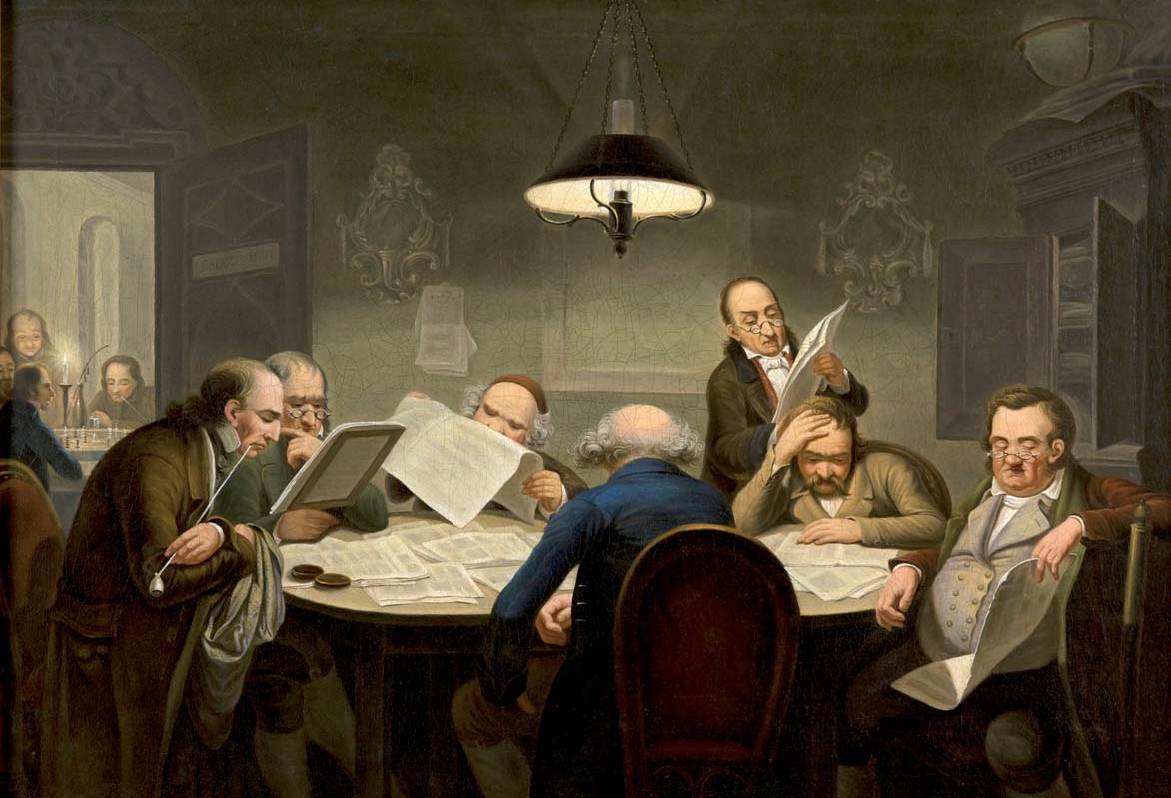
\includegraphics[width=1\textwidth]{images/intro/Lesegesellschaft.png}
	\caption[Caption for LOF]{Johann Peter Hasenclever: \textit{Das Lesekabinett} (The Reading Society), 1843.\protect\footnotemark}
	\label{fig:lesegesel}
\end{figure}

\footnotetext{\url{https://commons.wikimedia.org/wiki/File:Lesegesellschaft,_um_1843.png}}

The audience is limited when discussing an issue in person. A way for a non-journalist to join the debate in a newspaper are \textit{letters to the editor}. Everybody can send their opinions in a letter to the editors of newspapers. Editors can then decide to print a selection. Until today, this is a common tool for newspapers to give voice to the ordinary people. However, it is rather unlikely that the letters are printed since space in a printed newspaper is sparse.
The introduction of the Web revolutionized media. News are now delivered online as well and the space restrictions of the Internet are more relaxed.
Since the era of so called \textit{Web 2.0}, users generate content themselves.
These developments established the \textit{comment section} as a special place on blogs, social media platforms or newspapers where users can leave their thoughts.

Figure~\ref{fig:nyt_article_comment} displays two typical comments on an opinion piece of the New York Times.

\begin{figure}[h]
\begin{tabular}{ll}
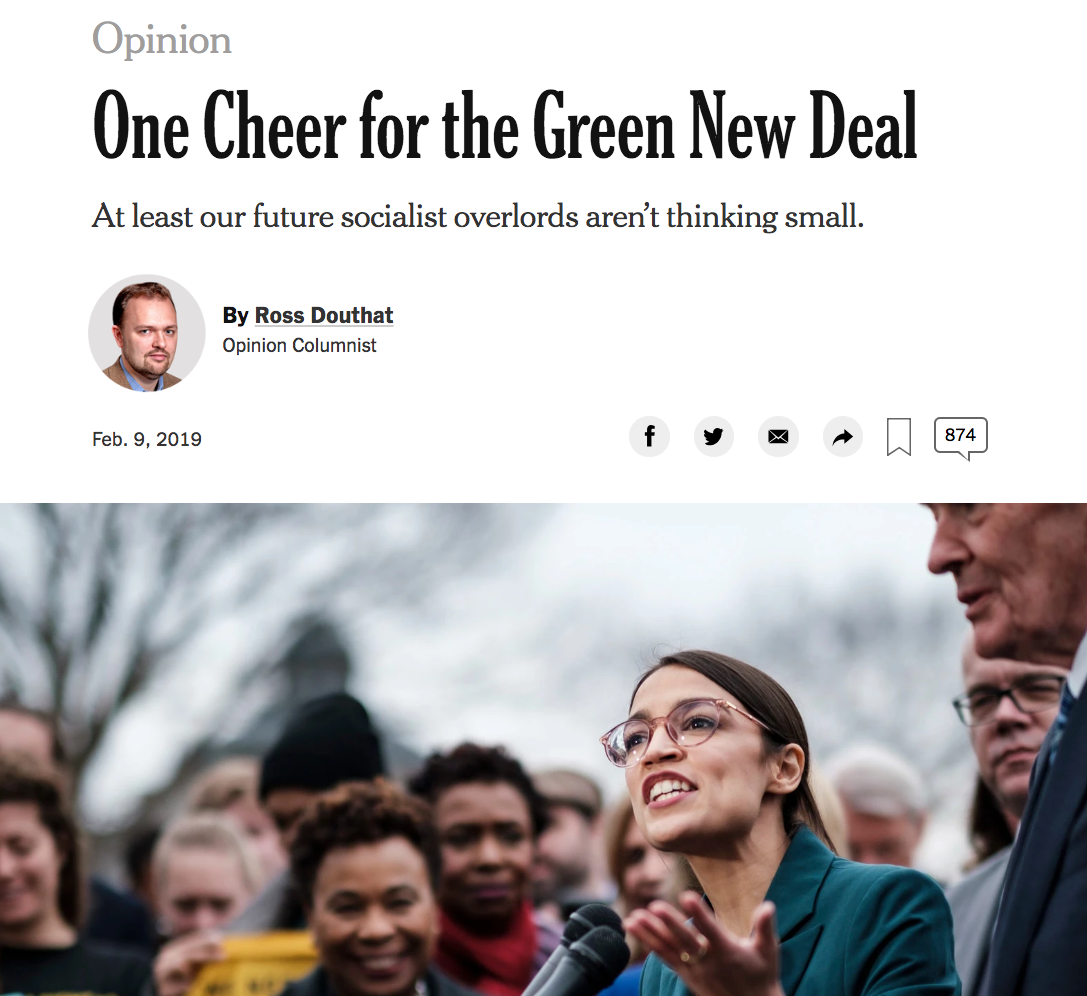
\includegraphics[width=0.6\textwidth]{images/intro/nyt_article.png}
&
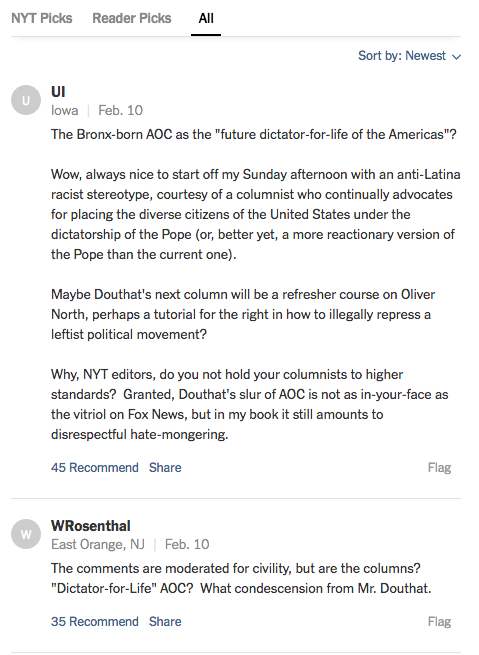
\includegraphics[width=0.4\textwidth]{images/intro/nyt_comment1.png}
\end{tabular}
\caption[Caption for LOF]{An option article of the New York Times received 878 comments before the comment section was closed.\protect\footnotemark}
\label{fig:nyt_article_comment}
\end{figure}

\footnotetext{\url{https://www.nytimes.com/2019/02/09/opinion/alexandria-ocasio-cortez-green-new-deal.html}}

In the beginning, comments were hailed as a democratization of the debate. In contrast to the previous unidirectional communication, the communication is now multidirectional. Readers can discuss an article with one another. They can also give new perspectives to an issue by contributing personal stories or adding expert knowledge on a specific subject. Furthermore, they hold journalists accountable as Glenn Greenwald\footnote{\url{https://theintercept.com/2017/12/18/comments-coral-project/}} states:

\begin{quote}
``Journalists often tout their responsibility to hold the powerful accountable. Comments are a way to hold journalists themselves accountable.''
\end{quote}

In addition, the introduction of online news comments was an emancipatory act of depriving journalists of their role as gatekeepers. For the first time, a debate was open for everybody with an Internet connection -- so almost everybody. This sets the idea of discourse ethics as proposed by J{\"u}rgen Habermas into practice.
The essence of this thought is the belief, that a collective by exchanging arguments can come to superior conclusions than a sole person.
This is a stark contrast to the prior philosophical idea of Immanuel Kant's categorical imperative which focuses on individuals' convictions. The concept of Habermas is vague and implementation-agnostic but there are certain rules to follow. One rule, i.e., declares that arguments must not be repeated. And he promises if all participants obey the rules, the community will eventually reach a common conclusion which then manifests the morale. So in the best case, readers discuss an issue under an article and in the end, all participants share the same opinion.
Nevertheless, this in an idealistic scenario and Habermas did not have news comments in mind when he developed the idea in the beginning of the 1970s.
In the following, we examine the current problems of news comments and show that repeated arguments may not the biggest one.

\begin{figure}[h]
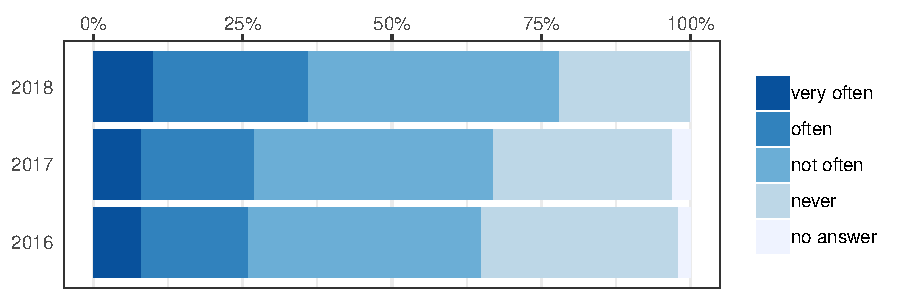
\includegraphics[width=1\textwidth]{graphs/hate_on_the_web/hate_paper.pdf}
\caption[Caption for LOF]{"Have you witnessed hate speech or hast posts on the Internet?". This question is part of a survey among 1000 Germans by the \textit{Landesanstalt Medien NRW}.\protect\footnotemark}
\label{Fig:hate_on_the_web}
\end{figure}

\footnotetext{\url{https://www.medienanstalt-nrw.de/fileadmin/user_upload/lfm-nrw/Foerderung/Forschung/Dateien_Forschung/forsaHate_Speech_2018_Ergebnisbericht_LFM_NRW.pdf}}

Online news outlets are drowning in the vast quantity of user comments. While there are certainly high-quality comments that follow the high hopes of emancipation, there are also comments which are rather unwelcome. They range from out-of-topic discussions to the use of offensive language. A survey by the \textit{Landesanstalt Medien NRW} among German Internet users is shown in Figure~\ref{Fig:hate_on_the_web}. The survey reveals that users increasingly witness hate on the Web. To remove problematic comments, the comment section needs to be moderated. But the moderation process involves specially trained humans who decide about the existence of comments. Consequently, newspapers abolish their comment section altogether. The biggest German daily newspaper, \textit{Sueddeutsche Zeitung}, closed their comment section in 2014 as one of the earliest newspaper\footnote{\url{https://www.freitag.de/autoren/jan-jasper-kosok/die-sz-schliesst-ihre-kommentarfunktion}}.

In 2016, a survey\footnote{\url{https://netzpolitik.org/2016/umfrage-zeitungsredaktionen-schraenken-kommentarfunktionen-2015-weiter-ein/}} among German news outlets showed that two in five restricted commenting on their website.
Although moderators could help, they are expensive and the news industry already has economic problems and is on a decline.
In Figure~\ref{fig:decline_of_newspapers}, two graphs illustrate the problem on the example of the US news sector. The number of employees was almost cut by half from 2004 to 2017. In mid 2000s, the advertising revenue decreased rapidly. One reason are ad-blocking tools for users to hide advertisement to increase the overall user experience. Another reason are new, strong competitors in the online advertising market. The Internet enables new and more creative forms of advertisement with, e.g., Google's AdWords or influencers on Instagram.
The news sector is in a ambivalent state.
While recent technological development allows novel ways of storytelling with, i.e., interactive graphics, decreasing revenue streams, that go along with it, remain an open problem.
Solving it is out of scope of this master's thesis but Natural-Language Processing (NLP) using machine learning techniques promises to improve efficiency in managing news comments.
As a consequence, less manual moderation is required so the comment sections remain open which fosters our democracy.

\begin{figure}
    \centering
    \subfloat[Employees in the US news sector.\protect\footnotemark]{{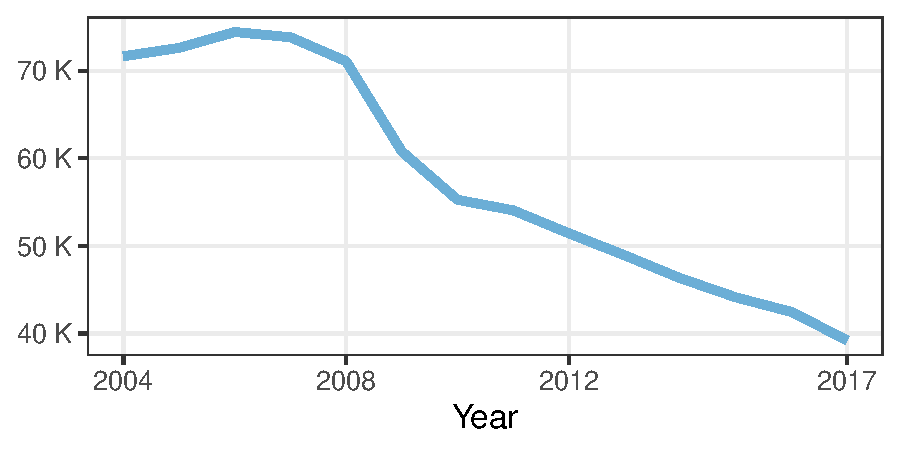
\includegraphics[width=0.5\textwidth]{graphs/decline_of_newspapers/emp_paper.pdf} }}
    \subfloat[Revenue in the US news sector.\protect\footnotemark]{{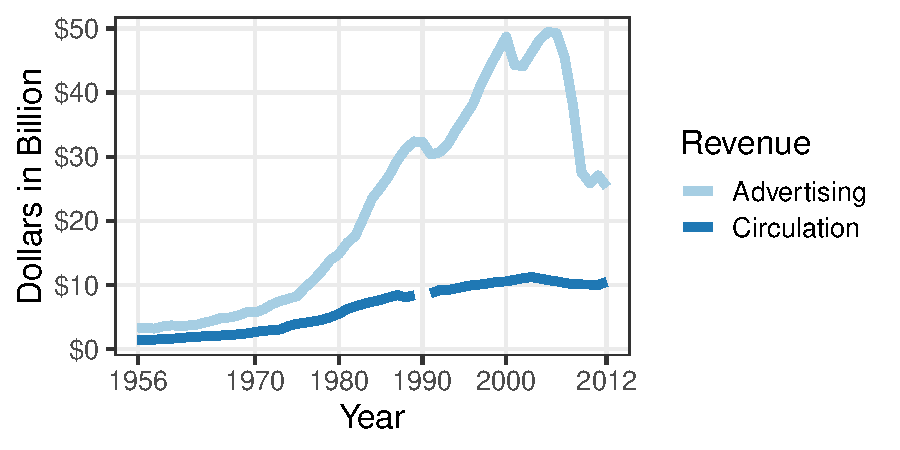
\includegraphics[width=0.5\textwidth]{graphs/decline_of_newspapers/rev_paper.pdf} }}
    \caption{The decline of the US news sector at the example of number of employees and revenue.}
    \label{fig:decline_of_newspapers}
\end{figure}

\footnotetext{Source: Pew Research Center analysis of Bureau of Labor Statistics Occupational Employment Statistics data.}
\footnotetext{Source: News Media Alliance, formerly Newspaper Association of America (through 2012); Pew Research Center analysis of year-end SEC filings of publicly traded newspaper companies (2013-2017).}

 There already exist works to automatically detect hate speech or abusive language in user-generated content~\cite{hateoffensive, Nobata:2016:ALD:2872427.2883062, risch_delete_nodate, schmidt2017survey}. In this work, we focus on classifying comments in a more general way.
Comments are assigned to different categories. For instance, what the sentiment of a comment is or whether it is off-topic.
It can be any criteria for classification.
This classification can aide comment moderators and also creates new opportunities for other features. For instance, comments are currently mainly ranked chronologically or based on their up- and down-votes. The classification of comments allows to rank them by specific criteria. A feature which is enabled by classification are comment filters. One could choose to hide a specific kind of comments. This is already in production on social media platforms such as Twitter or Facebook. They automatically hide low quality or unpleasant comments. With a fine-grained comments classification, one could think of even more possibilities. For example, a user is tired of negativity and only wants to read comments with a positive sentiment.

In contrast to prior work, we assume that the article's context, namely, the whole conversation, is essential to make a classification of a single comment. The article acts as a conversation-starter and the comments leading up to the comment are the conversation partners. To illustrate our motivation, we take two humanly-annotated comments from a Canadian newspaper~\cite{kolhatkar2018sfu}:

\begin{quote}
    ``Time for the elders and chiefs to stand up to the plate and take a leadership role!''
 \end{quote}

This comment is labeled as constructive (or in other words: high-quality) and
\begin{quote}
    ``Maybe this will motivate the cabbies in TO to clean their filthy cars! That are a disgrace.''
\end{quote}

is labeled as non-constructive. For humans, it is hard to make a judgment without reading the corresponding article and previous comments first. Moreover, the annotators were required to read the article first before deciding whether an article is constructive. So we should be fair and also give the machine the possibility to obtain the context before classifying.
The term `context' describes different aspects in this domain.
One could also think of context by considering a commentator's previous comment history.
While this would probably help to improve the performance of a classifier, it is unfair.
A classification of text should depend only on a very comment.
We illustrate this differentiation using following example.
In a fair judicature, a conviction must be based on clear evidence not on the criminal history.
The history only matters for determining the sentence.
This should apply for the classification of comments as well: only the current text is important, neither previous comments nor misbehavior.
Also from a privacy perspective it is important to point out, that creating information about users means profiling them.
Storing personal information has further implications since they are under severe protection with the European Union General Data Protection Regulation (GDPR) in force.
It is recommended to only store personal information when it is absolutely necessary.
For this work, we do not use any user information for classification.

In order to formally define the problem of conversation-aware classification, let $C$ and $A$ be the set of all comments and articles respectively.
In addition, we define:
\\\\
$\text{isArticle}=\{(c, a)| \forall (c,a) \in C \times A: c\text{ is a comment of }a\}$
\\
$\text{isPrevious}=\{(c, o, a)| \forall (c,o, a) \in C \times C \times A:\text{isArticle(}c, a\text{)} \wedge \text{isArticle(}o, a\text{)} \wedge \\  c_{time} > o_{time}\}$

The training set $T =\{(c_n, a_n, s_n, y_n)\}^N_{n=1}$ consists of quadruple-wise data, where $c \in C$, $a \in A$, $s \subseteq \{o | \forall o \text{ isPrevious(}c,o,a)\}$ and $(c, a) \in \text{isArticle}$.
Further, $y \in Y $ is the corresponding label for $Y=\{1,\dotsc, l\}$ classes.
We wish to train a classifier $\gamma$ that maps a comment, its article, and its previous comments (in the conversation) to classes: $\gamma: C \times A \times C^* \rightarrow Y$.

The field of journalism is tightly coupled with the technological advancement of our society. As mentioned earlier, only through the printing press could humans spread information so fast. This allowed the journalistic profession to establish and flourish. The ongoing digital revolution also affects journalists and there is a long tradition of supporting their work with digital technologies. It started in the late 1960s with computer-assisted reporting and lead to current ideas about automatic reporting. Right now, there is a larger effort by supporting newspapers in managing their user comments. On example is the unprecedented Coral Project\footnote{\url{https://coralproject.net}}, a cooperation among Mozilla, the New York Times, and the Washington Post, that interviewed more than 400 experts in 150 newsrooms to develop an IT system to manage comments. Research on news comments or other user-generated content is done extensively in other research fields. For instance, there exists research on news comments in the field of communication studies. Recent work by Ksiazek and Springer~\cite{eldridge_ii_user_2018} gives an overview over current trends and future directions in this area. The increasing hate in the comment section is one object of investigation. Besides, there is a multitude of publications that highlight the importance of a comment's context. Loosen et al.~\cite{loosen_making_2017} formulated several comment quality indicators after conducting interviews with news professionals as well as developing a software mockup. Among other things, they list `reference to the article' and `references to other comments' as an indicator for high-quality comments. Their work is built upon earlier research done by Diakopoulos et al.~\cite{Diakopoulos:2011:TQD:1958824.1958844} and Noci et al.~\cite{noci2012comments} who also investigate characteristics of comments. The relation of one comment to other comments or the article itself plays a role when looking at the perception of comments. There is also an abundance of comment guidelines that describe comments that newspaper desire. The New York Time writes in their guidelines\footnote{\url{https://help.nytimes.com/hc/en-us/articles/115014792387-Comments}}: ``We are interested in articulate, well-informed remarks that are relevant to the article.'' Also, the community guidelines by the Guardian requires commentators to ``keep it relevant''\footnote{\url{https://www.theguardian.com/community-standards}}.
So, the relation of comment to the article and previous comments is important to consider. Machine learning methods ought to respect the knowledge generated in non-computer-science fields and try to include them into their own work.

This thesis is structured as follows. In Section~\ref{ch:related_work}, we give a detailed overview of related scientific work before providing background information in Section~\ref{ch:background}.
In Section~\ref{ch:datasets}, we describe the datasets we conduct experiments on.
In Section~\ref{ch:approach}, we present our contributions and evaluate them in Section~\ref{sec:evaluation}.
Finally, we conclude in Section~\ref{chp:conclusions} and give an outlook for future work.



\chapter{Related Work}
\label{ch:related_work}

The related literature can be split into two categories. Section~\ref{sec:classnews} is about the classification of news comments. While for some approaches consider the context, i.e., an article's title, it is only one feature among others. The comment is not considered embedded in a whole conversational context. This is different to approaches presented in Section~\ref{sec:contextawaretext}. There the exploitation of the sequential or tree-structures of online discussions is the principal motivation.

\section{Classification of News Comments}
\label{sec:classnews}

With the beginning of Web 2.0, there is an abundance of user-generated content freely accessible. Some influential earlier work analyzed comments on Digg\footnote{\url{https://digg.com}}~\cite{Gomez:2008:SAS:1367497.1367585, Lampe:2004:SBD:985692.985761}, or predicted the popularity of online content on YouTube\footnote{\url{https://youtube.com}} and Digg~\cite{Szabo:2010:PPO:1787234.1787254} or Reddit\footnote{\url{https://reddit.com}}~\cite{Rizos:2016:PNP:2872518.2890096}. The analysis of news comments is a subset of the research done on user-generated content so it falls in this line. But we focus on news comments so the remaining section is dedicated to them.

Coming from the area of Human-Computer Interaction (HCI), Park et al.~\cite{Park:2016:SCM:2858036.2858389} build an IT system to support moderators to identify high-quality comments. They incorporate traditional, feature-based machine learning. Besides other components, they automatically assign a quality score to each comment. They hand-crafted various features based on a comment's text as well as metadata. For instance, they consider a comment's text as well as the commentator's history. The authors tried to measure the distance of a comment's text to the article's text and other comments' text as \textit{relevance} of a comment. This relevance metric originates from work by Nicholas Diakopoulos~\cite{Diakopoulos:2015:EEC:2675133.2675160}. He uses a simple tf-idf~\cite{salton1986introduction} model to create vector representations of comments and articles to use, i.e., cosine distance to measure similarity amongst comments or between an article and a comment. This metric has serious short comings since it only considers identical words matches. So for instance, the heavy use of synonyms results in a comment to be marked as irrelevant to an article. However, for Park et al. the machine learning part is not the focus of their work. They simply demonstrate what can be built by applying NLP and machine learning to news comments. In this sense, well-functioning machine learning techniques, such as classification, are a necessity for those end-to-end systems. Park et al. conclude in their section that more research in the area is required.

A similar work by H\"aring et al.~\cite{haring2018addressed} focusses on the classification of German \textit{meta-comments}. Meta-comments are comments that, i.e., address an article's authors directly. So they are not about the topic of an article but \textit{meta}, so meta-comments. In cooperation with a large German newspaper, they highlight the need for journalists to identify those comments. Journalists only have a limited amount of time so they want to spend it wisely. For the classification, they experiment with various traditional manually engineered features. They also conduct qualitative research about identifying also characteristics of those meta-comments. The author's research is only touching machine learning with NLP since it is published at a HCI conference. They also tried to use neural models but traditional machine learning methods outperformed them. They conjecture that the number of annotated data with only a couple hundreds samples is too few. They do not use any conversation or context-aware methods. Only the news department of an articles is considered. Besides proprietary data, they use the research dataset \textit{One Million Posts} by Schabus et al.~\cite{Schabus:2017:OMP:3077136.3080711} consisting of Austrian comments. The authors constructed a dataset of one million unlabeled comments and annotated a view thousand of them. They present several approaches and experiment with feature-based machine learning as well as deep learning. On two out of eight categories a Long short-term memory network (LSTM)~\cite{Hochreiter:1997:LSM:1246443.1246450} achieved the best $\text{F}_{1}$ score. In their follow-up paper, Schabus and Skowron~\cite{schabus_academic-industrial_nodate} describe how they resort to a feature-based machine method for usage in a production system. They also experiment with including features related to the headline of category of the article but could not get good results. They focus on the implementation of a news comment classification system. While they report baselines, that point out that there are only baselines. Their $\text{F}_{1}$ scores range from about 0.15 (positive comments) to about 0.7 (personal stories) so there is still room for improvement. They also point out the difficulties of news comment classification since comments are much more ``diverse in terms of topic, style, length, author intention [..]'' than movie reviews. Detecting sentiment in movie reviews is a common problem setting for NLP research.

News organization realized that high-quality comments are easily overlooked in the vast amount of comments. Even though the community votes on comments, those comments with the most up-votes are not necessarily the ones with the highest quality. Thus, moderators pick comments themselves. On the New York Times\footnote{\url{https://www.nytimes.com}} (NYT) website,  those comments are called \textit{NYT Picks}. Since these comments went through a selection process, one can think about it as a binary classification problem. This caught the interest of research to investigate the characteristics of picked and non-picked comments. But in this kind of post-hoc analysis, it is hard to understand the reasoning process of the moderations and other external factors. It is also more than likely that different people picked and the selection process varied over the time. Altogether, this annotation process is very opaque. Nevertheless, research was working with it. Nicholas Diakopoulos~\cite{diakopoulos2015picking} presents nine criteria for comments that distinguish NYT Picks from non-NYT Picks and three of them can be computed: Brevity, Readability, and Personal Experience. For the other six, Diakopoulos paid crowd-annotators to classify them and found significant differences between picked and not picked ones. One finding is that comments are more likely to get picked shorty after the release of an article. However, this could also be explained with the selection process of moderators. Maybe they were following the debate in the comment section more closely in the beginning. The authors' work falls more into the area of communication but even there their finding are to question due to uncertainty around the selection process.

Kolhatkar and Taboada~\cite{kolhatkar_using_2017} try to automatically identify constructive comments. They define constructive as follow:
\begin{quote}
     ``Constructive comments intend to create a civil dialogue through remarks that are relevant to the article and not intended to merely provoke an emotional response. They are typically targeted to specific points and supported by appropriate evidence.''
\end{quote}
Since there is a scarcity of labeled annotated comments, they used the NYT picks in a creative way. They are aware of the fact that it is hard to draw conclusion from the non-picked comments. So they only consider the picked comments and define them as constructive. These are the positive samples. As negative, they resort to another dataset about news comments, the Yahoo News Annotated Comment Corpus (YNACC)~\cite{napoles2017finding}. The YNACC contains annotations on comment-level as well a thread-level. One category for the classification is constructiveness. So Kolhatkar and Taboada choose all comments from non-constructive threads as the negative samples.
They conduct experiments on several model variations. They report results on yet another set of annotated comments that they published as the SFU Opinion and Comments Corpus (SOCC)~\cite{kolhatkar2018sfu}.
However, they were mainly focusing on traditional feature-based machine learning. They were using some simple length features, e.g, comment length and average word length, and achieved an $\text{F}_{1}$ score of 0.79. They were unable to push the score further with more features. With other more complex features argumentation, text quality, and named entity features, they achieved an $\text{F}_{1}$ score of 0.84. They also investigated approaches based on deep learning, a bidirectional LSTM, and received a $\text{F}_{1}$ score of 0.81. The number of training samples with about 30k should be sufficient to outperform traditional machine learning. However, it did not beat the feature-based machine learning approaches on the test set. But their values are only on the SOCC dataset which is used as test set. And those comment stem from another newspaper than the comments the model was trained one. When looking at the validation set, the LSTM outperformances all other approaches with an $\text{F}_{1}$ score of 0.86 and 0.83 on the second place. The comments in the training and validation set are from the same newspaper.
So the results should be interpret carefully. In their follow-up work, Kolhatkar and Taboada~\cite{kolhatkar2017constructive} predicted the comments in the SOCC with an accuracy of $72.59\%$ by using an LSTM.
This must also be taken with caution since the number of samples is relatively low (1k).

The aforementioned YNACC dataset was in the focus of the work of Napoles et al.~\cite{napoles2017automatically}. They identified constructive threads among 2.4k annotated threads. The major focus of their work is traditional machine learning. They employ traditional feature engineering. Furthermore, they use features of the comment's text as well as features of the user such as commenting history and also user contributed up- and downvotes. They compare several results, also a neural model. The best performing model is a pipeline model that comprises several steps of features created from a comment's text as well as metadata. They achieve a $\text{F}_{1}$ score of 0.73 on the test set of the YNACC data and $\text{F}_{1}$ score of 0.91 on another external dataset of an online discussion forum. Even if the numbers on the external datasets sound impressing, no significance testing was applied. Since the datasets with about 1k samples is, once again, relatively low, the results may be created by chance. And it is not clear on how many different external datasets the model was tested. Maybe it was tested on 10 different datasets, and it performed well on only one datasets and so the results may be cherry-picked. Also it is not clear how difficult the classification of this external dataset it. Maybe a simple baseline could have achieved even better results. So while the paper shows the performance of certain features, the results have to be interpret carefully.

In this section, we briefly introduced research datasets of annotated news comments. A detailed comparison of all available datasets is presented in Section~\ref{sec:datasets_comments_table}.

\section{Conversation-aware Text Classification}
\label{sec:contextawaretext}

In this section, we present text classification approaches that exploit sequential or tree structures of text. This is often the case on social media platforms with their nested comment structures. The conversation is often started by a particle item, such as a news article or a social media post. This starts an online conversation where subsequent comments are part of this conversation.

Cheng et al.~\cite{2018arXiv180807191C}\footnote{This publication was not formally published and is only a pre-print. We still consider it relevant because it is recent and closely related to our (niche) topic.} consider the abstract of the news article as well as surrounding comments to classify comments. It adapts the text matching approach that uses an LSTM with attention mechanism. They describe text matching as a general problem to decide whether two text relate to each other in some way. In this sense, question answering or duplicate detection are a special case of a text matching. In this case, the text matching is done between a comment and surrounding comments as well as a comment and article's abstract and title. The text is represented by Word2vec embeddings~\cite{DBLP:journals/corr/abs-1301-3781}. The text matching computations are combined  in a final layer. Then then a comment gets classified. However, the paper has one weakness. They interpret all comments with over 10 up-votes as positive and the rest as negative samples in a binary classification problem. This is a gross simplification. For instance, earlier comments are more likely to get more up-votes. So they may only predict comments that appear earlier in the discussions than others. Furthermore, certain topics attract more people and thus receive more votes. So there is no justification for the number of 10 up-votes. In order to use the votes as labels, one has to normalize the up-votes and down-votes. The social media platform Reddit has implemented a system to normalize upvotes since time since posted. Even though the authors achieved an accuracy of $70.75\%$ and a $\text{F}_{1}$ score of $0.8073$, their true contribution is unclear.

\newpage

Covering the related work on hate speech detection is out of scope for this paper. But there is one particular paper by Gao and Huang~\cite{Gao_2017} that is closely related because they work on context-aware classification.
They as well point out that work on comments neglects its context. They developed an architecture of three parallel LSTMs, one for the text, one for the author, and one for the article. Those three LSTMs are combined into a final layer before classifying. They as well used pre-trained Word2vec embeddings for text representation. They constructed their own datasets of annotated tweets that relate to news articles. In their experiments, they claim that their context-aware model outperforms the one without context. Unfortunately, they did not apply their method to a commonly used dataset to put their contribution into perspective.
 \begin{figure}
  \begin{center}
    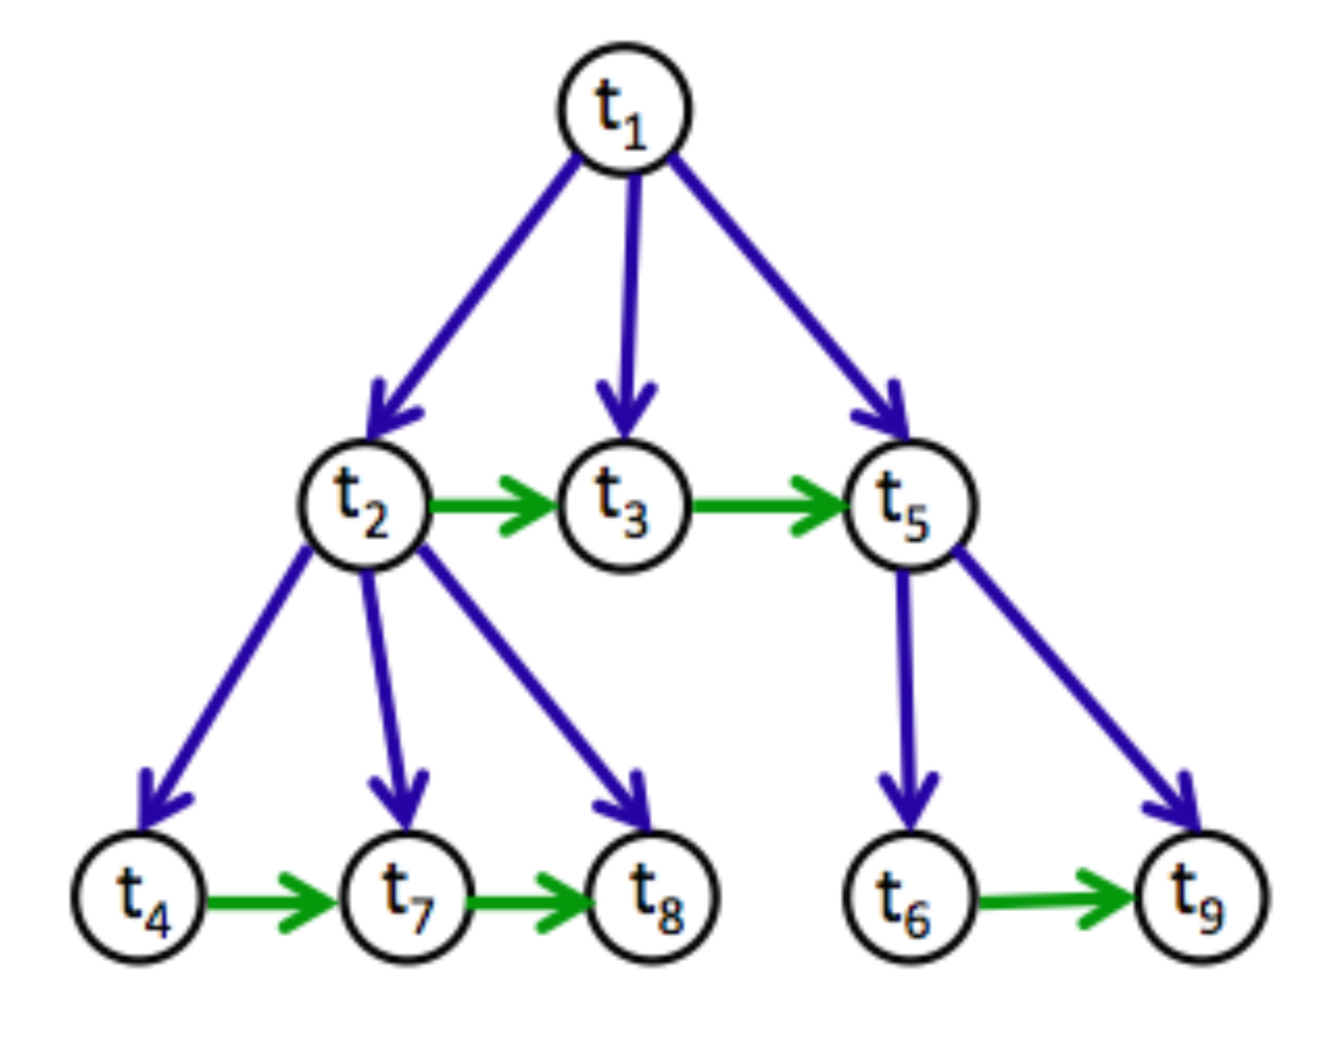
\includegraphics[width=0.4\textwidth]{images/related_work/conversial_modelling.png}
  \end{center}
  \caption{The Graph structure gets introduced to the LSTM with two different previous time steps. The figures is taken from the original paper by Zayats and Ostendorf~\cite{Q18-1009}.}
   \label{fig:zayats_tree} 
\end{figure}

A new LSTM cell by Zayats and Ostendorf~\cite{Q18-1009} intends to exploit the graph structure of the data. They add an additional previous time step. So there is one previous time step for the hierarchy and one for the time. The two different steps are illustrated in Figure~\ref{fig:zayats_tree}.
 To evaluate their contribution, they predict community votings on Reddit comments. With their approach, they outperformed context-agnostic approaches in their work. To represent their text, they used Word2vec embeddings. They did not evaluate their approach on other text classification tasks. Since the votings has some uncertainties as already mentioned earlier, the benefit of this LSTM modification is uncertain. Miura et al.~\cite{C18-1322} conducted additional experiments with this LSTM cell. But they used Reddits comments that were annotated for their role in the discourse.
 The dataset is named Coarse Discourse~\cite{coarsediscourse} and it will be described in the next paragraph.
So it was different setup and the results were below other more traditional machine learning approach of a conditional random field. They hypotheses that predicting user votes is a special kind of problem setting where the text is not a major factor. Other features such as the timing of a comment plays is more important. So this cell is not suited for text classification and thus not for news comments classification.
\begin{figure}
  \begin{center}
    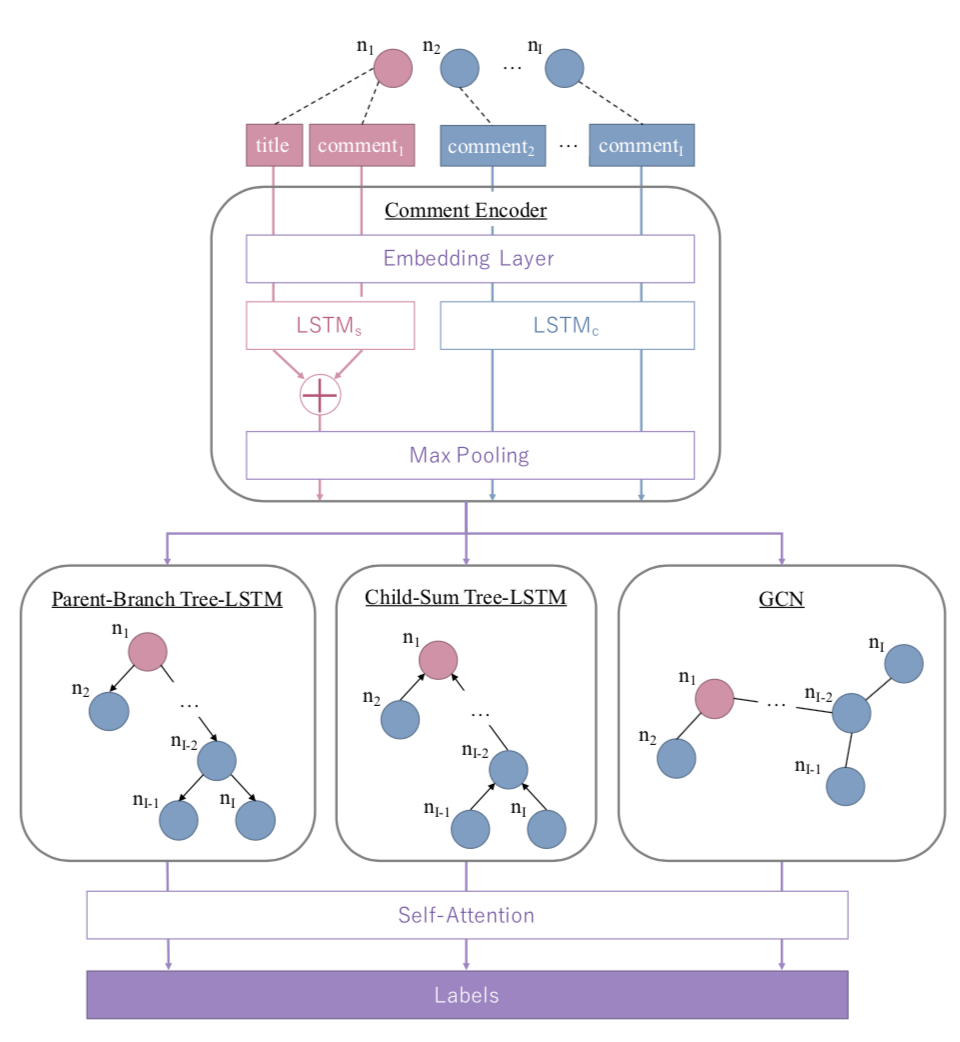
\includegraphics[width=0.7\textwidth]{images/related_work/integrating_tree.png}
  \end{center}
  \caption{The architecture of integrating tree-structures for text classification. The figures is taken from the original paper by Miura et al.~\cite{C18-1322}.}
  \label{fig:integrating_tree_structure}
\end{figure}

% Firstly und Secondly benutzen sehr viele Deutsche. First und Second ist auch voll okay.
\newpage

The aforementioned paper by Miura et al.~\cite{C18-1322} presented a new graph-based text classification architecture. Overall the architecture is quite complex as visualized in Figure~\ref{fig:integrating_tree_structure}. First, the comments are encoded into an internal representation. There is the different handling of the first comment (and its title) and all other comments. Second, the comments are given into three context-aware sub-networks before getting concatenating again. To evaluate the performance of their architecture, they conduct experiments on a research dataset of annotated Reddit comments by Zhang et al.~\cite{coarsediscourse}. For text representation, they train Word2vec on a millions of Reddit comments. They achieved higher results than previously reported. The Reddit comments are annotated for their role in a discourse. For instance whether a comment is question or answer. This setting is called \textit{discourse classification}.

Another related problem is \textit{stance detection}. In this field, it is about detecting whether a response to a statement is affirmative or opposing. For this, Kochkina et al.~\cite{kochkina2017turing} introduced Branch-LSTM. They worked with tweets and split the structure into branches. Branch gets created by iterating over all branch nodes of the discussion tree. For each leaf, one goes all the way to the root. This sequence is called branch. The branches are then given as input to the network. For representing the text, they also use Word2vec but average the word embeddings for each comment. A simple averaging is too limiting to capture the nuances of a text~\cite{rueckle:2018}.
 Stops words or commons words such as forms of `be' or `have' appear often and distort the whole meaning that should be added with word embeddings.
In addition, they use various other hand-crafted features to enrich the tweet representation. There exist various similar ideas by Zubiga et al.~\cite{C16-1230, ZUBIAGA2018273} which has several works for the conversation.
There is also a different problem setting of identifying sarcasm in text.
Ghosh et al.~\cite{W17-5523} identified the role of conversation in this domain.
But they only encoded one previous post for each other post.
This is quite limiting since a conversation spans among multiple comments.
In addition, research on user product reviews is related field.
In it, there are as well approaches that take the context of a product review into consideration.
For instance, Zheng et al.~\cite{Zheng:2017:JDM:3018661.3018665} encoded the product description as well as reviews with an LSTM respectively before combining the two sub-networks into a classifier.

So there exists quite a lot of work on news comments as well as incorporating the conversation for the classification. But all of them a rather simplistic text representation of traditional word embeddings. In the next section, we will give background information on how text representation are derived from language models. They show superior results on various NLP tasks.


\chapter{Background}
\label{ch:background}

In this section, we give background information about recent development of NLP research as well as metrics we use for our experiments.
Transfer learning with language models achieve state-of-the-art results on text classification.
Thus we use them for our work.

\section{Transfer Learning in Computer Vision and Natural-Language Processing}

Transfer learning is a research problem about re-using computation resulting from one problem to another problem. The survey of Pan et al.~\cite{pan2010survey} gives an overview over field as of 2010. With the `third wave' of artificial neural networks, the field of machine learning changed dramatically and thus transfer learning as well. With AlexNet~\cite{NIPS2012_4824} dramatically outperforming all other approaches in the 2012 ImageNet challenge, it started the revitalization process of neural models. Besides technological progress, one reason for the sudden success were large publicly available annotated research datasets such as ImageNet~\cite{imagenet_cvpr09}.
More data allowed to train deep networks with more layers networks (`deep learning'). In addition, these datasets gave a new perspective onto transfer learning in computer vision (CV). Nowadays, pre-trained ImageNet models are available in many open source libraries. And it is extremely common to fine-tune only a fraction of the weights as demonstrated by Oquab et al.~\cite{Oquab_2014_CVPR}. Mostly, only the last layers are trained because the early layers only learn very basic features such as edges as shown by Yosinski et al.~\cite{Yosinski:2014:TFD:2969033.2969197}. Consequently, transfer learning in CV allows to apply large neural models with millions of parameters even on small dataset sizes.

While in CV transfer learning is pre-dominate it was not used as often in NLP. There has been some progress however. Word2vec~\cite{Mikolov:2013:DRW:2999792.2999959} introduced word embeddings that are trained on large corpora in order to project words into a vector space. The resulting embeddings can be used on other task since they bring `meaning' to text. The idea of pre-trained word embeddings was especially popularized by pre-trained FastText embeddings available in 157 languages~\cite{grave2018learning}. FastText embeddings~\cite{TACL999} are adapting the idea of Word2vec but take sub-word information into consideration. However, the effect of word embeddings for neural networks is limited due to the following reasons: First, since one word can have multiple meanings (polysemy) a single vector is not enough to characterize it. For instance, `bank' can describe a financial institution or an embankment. The true meaning in a sentence can only be inferred by considering the context. Second, the message of a sentence can also depend on the context. Irony or satire are hard or impossible to grasp when only looking at individual words. Third, when using embeddings with neural networks, typically the embedding is used only for the first layer. Subsequent, deeper layers do not have access to the `meaning' of a word that was injected through the word embeddings.

A successor of word embeddings are text representations derived from language models. First we give background information on language models and where they were used originally.

\section{Language Modeling}

The research problem of creating a language model (LM) is, as the name suggests, about abstracting an entire natural language into a model.
Instead of formulating rules to describe the construction of a language, the model should capture it by showing a collection of natural language text. There are different ways of defining the problem. One can work on the level of sentences, word n-grams, words, sub-words or characters. We focus on words in this section. We also limit ourselves to modern neural network models since they greatly outperform traditional approaches.
For a comprehensive introduction, the interested reader is advised to read Chapter~9 of the book by Goldberg and Hirst~\cite{Goldberg:2017:NNM:3110856}.
Bengio et al.~\cite{Bengio03aneural} define LM in their seminal work as follows:
\begin{equation*}
 P(w_{1}^{T})=\prod_{t=1}^{T} P(w_t|w_{1}^{t-1})
\end{equation*}
where is the $t$-th word, and writing sub-sequence $w_{i}^{j} = (w_{i}, w_{i+1},\ldots, w_{j-1}, w_{j})$. This means that the probability of a word depends on all previous words. All previous words can mean a lot of words when the LMs, i.e., is trained on books. For the purpose of simplification, the first approaches worked with a fixed size window. In another groundbreaking work, Mikolov et al.~\cite{conf/interspeech/MikolovKBCK10} used a recurrent neural network (RNN) to circumvent the fixed window size and Sundermeyer et al.~\cite{Sundermeyer2012LSTMNN} successfully applied LSTMs~\cite{Hochreiter:1997:LSM:1246443.1246450} to language modeling. LSTMs are a powerful variant of RNN because they can capture long-term dependencies in sequences but as well `forget' previous input sequences. However, since LSTM are strong but contain a lot of parameters, they are known to overfit. Merity et al. introduced AWD-LSTM~\cite{merityRegOpt} that use a lot of regularization to overcome overfitting. As of this writing, AWD-LSTM variations still hold various state-of-the-art results on LM competition datasets\footnote{\url{http://nlpprogress.com/english/language_modeling.html}}.

LMs are used, e.g., for spell correction, optical character recognition, keyword prediction, or speech recognitions. As a byproduct they also embody a text representation that considers longer sequences of text. This is presented in the next section.

% mb remove
\newpage

\section{Transfer Learning with Language Models}
\label{sec:bgrd_tlwlm}

The idea of using LMs for text representation is not fundamentally new. As early as 2008, Collobert and Weston~\cite{Collobert:2008:UAN:1390156.1390177} demonstrate how they used LM as an auxiliary task for other downstream tasks. But only the ELMO (``Embeddings from Language Models'') embeddings by Peters et al.~\cite{peters2018deep} about ten years later popularized the idea. The basic principle works as follows.
The first task is to train a LM on a large text corpus.
The text does not require special annotations, although the arrangement of words in a text is a type of annotation itself. In such a manner, the model has to learn the nuances of a language over long sequences of text. After training a LM, its capabilities are transformed to other tasks such as text classification. The ELMO embeddings consider only parts of the internal state of the LM for further usage. Other approaches, i.e., ULMFIT~\cite{howard2018universal}, adopt the whole trained LM directly and only adds additional layers. ULMFIT will be explained more in detail in the next section. Both use LSTMs for the LM but ELMO operates on character level. There are two approaches based on the Transformer architecture~\cite{NIPS2017_7181}: the OpenAI transformer by Radford et al.~\cite{radford2018improving, radford2019language} and BERT by Devin et al.~\cite{devlin2018bert}. BERT improves the OpenAI transformer by allowing the model learn a language forth and backwards at the same time. This requires a different formulation of the language model problem but this is beyond the scope of this brief overview. Abkib et al.~\cite{akbik_contextual_nodate} use a character-aware LSTM-based LM to transfer-learn to named entity recognition. Peters et al.~\cite{peters_dissecting_2018} investigate the different capabilities of LMs. They show, i.e., that language models learn part-of-speech tagging implicitly. However, LM are not the only way to create context-aware text representation \cite{D18-2029, mccann2017learned}.
 But the current results suggest that they are superior.

\section{ULMFIT}

ULMFIT by Howard and Ruder~\cite{howard2018universal} is the acronym for ``Universal Language Model Fine-tuning for Text Classification''. As of this writing, the approach holds multiple state-of-the-art results on text classification\footnote{\url{http://nlpprogress.com/text_classification.html}} and sentiment detection\footnote{\url{http://nlpprogress.com/sentiment_analysis.html}}, i.e., on the IMDb dataset~\cite{maas2011learning}. Since publication, similar models such as the aforementioned BERT achieve state-of-art results on question answering. ULMFIT even with magnitude less parameters, is still undefeated for text classification.
In the ULMFIT paper, the authors point out that fine-tuning a LM to a smaller dataset is the crucial part.
LMs consist of millions of parameters and when training them on few samples, information may get lost fast (``catastrophic forgetting'').
 They use three techniques to circumvent it.
One technique they use is \textit{discriminative fine-tuning}.
It is about assigning different learning rates for each layer.
The earlier the layer in the neural network (closer to the input), the smaller the learning rate should be. In general, earlier layers learn fundamentals of the data while latter layers learn high-level features~\cite{Yosinski:2014:TFD:2969033.2969197}.
Another method used is \textit{cyclical learning rates} proposed by Leslie Smith~\cite{smith2017cyclical}.
Smith points out, that networks can be trained in less epochs by changing the learning rate of over time.
 Howard and Ruder argue that it is important to not fine-tune the LM for many epochs to avoid catastrophic forgetting and overfitting.
 Finally, they \textit{gradual unfreeze} the layers.
 Freezing layers means to not update the weights of certain layers.
 So unfreezing makes them trainable again.
 This special approach means that they do not unfreeze all layers at once.
 Instead, they progressively unfreeze layers starting from the final layer. So first, only the last layer is trained.
 Second, the last layer and second-last layers and so forth until the model is fully unfrozen.
 The authors state that only by the combination of these techniques, they could achieve high-scoring results.
 For the LM architecture, they use the already mentioned AWD-LSTM.
  First, they train a LM on a collection of high-quality English Wikipedia articles \textit{Wikitext103}\footnote{\url{https://blog.einstein.ai/the-wikitext-long-term-dependency-language-modeling-dataset}}~\cite{wikitext103}.
 After the general training of the LM, it requires fine-tuning to the specific domain.
 The LM is not powerful enough to hold the knowledge of the complete English language.
 Since language is different in each domain, they have to fine-tune the LM to the target domain.
 Then as the final step, a classifier is trained. For this, the LM architecture is augmented with two additional blocks of fully connected layers. The two different model architectures are visualized in Figure~\ref{fig:ulmfit_archi}.

\begin{figure}
    \centering
    \subfloat[]{{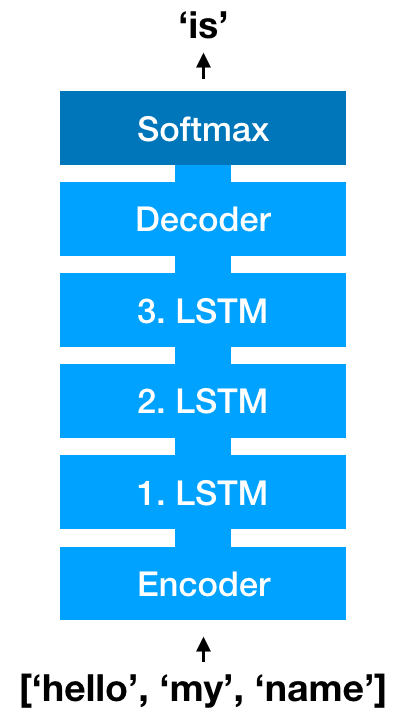
\includegraphics[height=150pt]{images/background/arch1.png} }}
    \subfloat[]{{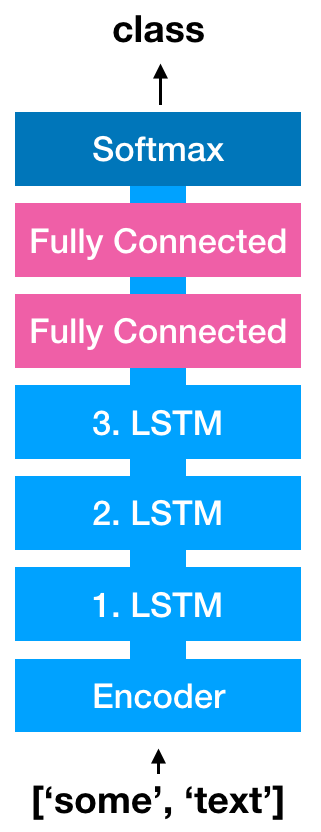
\includegraphics[height=173pt]{images/background/arch2_fixed2.png} }}
    \caption{The two different ULMFIT architectures. In Subfigure~(a) is the LM with a decoder to predict a news word. In Subfigure~(b) is the decoder replaced with two fully connected layers to predict a sample's class.}
    \label{fig:ulmfit_archi}
\end{figure}

The authors claim that even with only a small amount of annotated data, the classification achieves high results. Figure~\ref{fig:bgrd_ulmfit_res} demonstrates this at the example on IMDb movie reviews. This strength is particularly useful for newspaper, since resources to annotate data are scarce.

\begin{figure}
  \begin{center}
    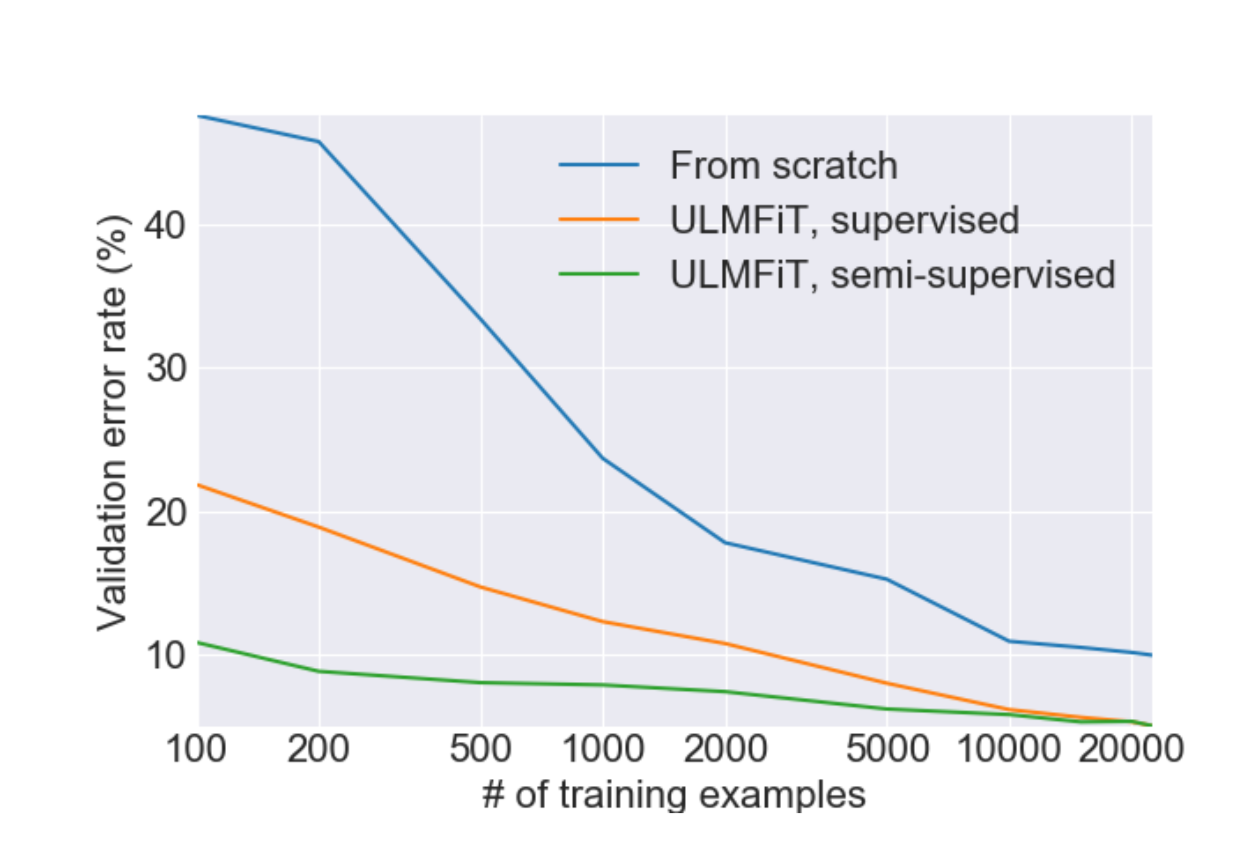
\includegraphics[width=0.6\textwidth]{images/background/ulmfit_results.png}
  \end{center}
  \caption{Validation error rates (lower is better) for ULMFIT on IMDb reviews. Semi-supervised means the LM is only fine-tuned on the according number of training samples whereas semi-supervised the LM is fine-tuned on all available samples. The figure was taken from the original paper~\cite{howard2018universal}.}
   \label{fig:bgrd_ulmfit_res}
\end{figure}

An implementation of ULMFIT is available in the Python deep learning library FastAI\footnote{\url{https://docs.fast.ai/text.html}} which itself is built upon PyTorch\footnote{\url{https://pytorch.org}}. It varies slightly from the original publication. The cyclical learning rate was originally not part of the paper but now the authors consider it as an integral part of the method.

%\newpage

\section{Classification Metrics}
\label{sec:metrics}

There is an abundance of metrics for classification. Sokolova and Lapalme give an overview~\cite{Sokolova:2009:SAP:1542545.1542682}. We briefly introduce those commonly used for news comment classification.

First, let us revisit precision, recall and $\text{F}_{1}$ score. With $tp$ as the number of true positives, $fp$ as the number of false positives, $tn$ as the number of true negatives, and $fn$ as the number of false negatives, precision and recall are defined as follows:

\begin{align*}
 \text{precision} &= \frac{tp}{tp+fp} & \text{recall} &= \frac{tp}{tp+fn} \\
\end{align*}

\newpage
The $\text{F}_{1}$ score is the harmonic mean of precision and recall:

\begin{equation*}
    \text{F}_{1} = 2 \cdot \frac{\text{precision} \cdot \text{recall}}{\text{precision} + \text{recall}}
\end{equation*}

In the original sense, precision and recall were compute in regard to one class. Hence, true positive and true negatives are calculated separately. But when using the metrics for classification, there is one drawback. The number of true negative samples are neither part of the precision nor recall formula.
Thus, these metrics do not lead to meaningful insights.
It is a problem when the majority class is treated as positive class.
In this case, it is easy to achieve high $\text{F}_{1}$~scores by simple always predicting the majority class (with a recall of 1 and high precision due being the majority class).
To overcome this, typically the scores are computed in regard to each class and then aggregated into a final score. There are three main types of aggregations: \textit{micro}, \textit{macro}, and \textit{weighted}\footnote{As implemented in the popular Python package scikit-learn.}. For \textit{micro}, the samples for true positives, false positives, etc., are counted across all classes and then the final score is computed.
For binary and multi-class classification, this is equivalent to the metric accuracy.
The accuracy is the share of samples there was assigned to the correct class.
For \textit{macro}, the scores are computed for each class separately and the intermediate scores are then averaged to a final score. \textit{Weighted} builds upon the macro-averaged score and weights them in respect to the number of samples per class.
Often micro and macro $\text{F}_{1}$~scores are used in conjunction to asses the quality of model.

Always using two metrics is cumbersome. To have a single metric that evaluates the performance of a model, we use Cohen's Kappa for this thesis.
Cohen's Kappa or short Kappa (or $\kappa$) was introduced by John Cohen~\cite{cohen_kappa_1960} and it was originally meant to measure the agreement among annotators.
However, it can be used as classification metric as well~\cite{ferri2009experimental,witten2005data}.

It is defined as follows:

\begin{equation*}
    \text{Kappa} = \frac{p_o - p_e}{1 - p_e}
\end{equation*}

$p_o$ is the observed agreement (accuracy) and $p_e$ is the expected agreement (accuracy by chance).
It takes into account whether classification results could happen randomly.
This is especially useful for imbalanced datasets, as it is often the case when working with real-life data such as news comments.


\chapter{Datasets}
\label{ch:datasets}

In this section, we first give an overview on the available datasets of annotated news comments. Afterwards, we describe chosen datasets in detail and reflect on the ethics of their creation process.

\section{Datasets of Annotated News Comments}
\label{sec:datasets_comments_table}

In Table~\ref{tab:datasets}, we list the characters of four datasets of annotated news comments. As of the writing, they are the only one available for research purposes.
Since we are not focusing on hate speech detection, we do not include comments datasets about hate speech here.
The interested reader is guided to the datasets section of the survey paper by Schmidt and Wiegand~\cite{schmidt2017survey}.

\begin{table}[H]
\small
  \caption{Four corpora of annotated news comments are available for research.}
  \begin{tabular}{| p{3cm} | p{1.5cm} | p{3cm} | p{5.5cm} |}
    \hline
    Dataset & Language & Unlabeled & Labeled \\ \hline
    SFU Opinion and Comments Corpus (SOCC) &  English & 10k articles, 663k comments from 303k comment threads & 1k comments in responses to 10 articles, labeled for constructiveness and toxicity \\ \hline
    Yahoo News Annotated Comments Corpus (YNACC) &  English & 230k comments from 34k threads under 2.8k articles (not included) & 9.2k comments labeled for agreement, audience, persuasiveness, sentiment, tone, off-topic (15 sub-classes)\\ \hline
        One Million Posts Corpus (OMPC) &  German & 12k articles, 1M comments & 11k comments with the following labels: sentiment, off-topic, inappropriate, discriminating, feedback, personal studies, argument used \\ \hline
        Tencent News Corpus (TNC) &  Chinese &  200K articles and 4.5M comments & 40k comments labeled for quality (from 1 to 5) \\ \hline
  \end{tabular}
  \label{tab:datasets}
\end{table}

Besides the labeled comments, all corpora contain a large number of unlabeled comments. This is helpful for our language-model-based approach. For our experiments, the Yahoo News Annotated Comments Corpus (YNACC) by Napoles et al.~\cite{napoles2017finding} and the One Million Posts Corpus (OMPC) by Schabus et al.~\cite{schabus_academic-industrial_nodate,Schabus:2017:OMP:3077136.3080711} are especially interesting. The number of annotated comments in the SFU Opinion and Comments Corpus (SOCC) by Kolhatkar et al.~\cite{kolhatkar2018sfu} is too small. The Tencent News Corpus by Qin et al.~\cite{2018arXiv180503668Q} has enough data but only one label for quality.
In addition it is in Chinese which makes it harder to work with the text, since we do not read it.
YNACC and OMPC have also some overlapping annotation criteria: off-topic and sentiment. This allows us to compare the same method with identical labels on both datasets.

\section{Yahoo News Annotated Comments Corpus}
\label{sec:datasets_ynacc}

First, we describe characteristics of the data and how it was annotated.
Then, we present reported values and speculate about used metrics. Finally, we explain required data cleaning steps.

\subsection{Description of the Dataset and Annotation Process}
\label{subsec:datasets_ynacc_description}

\begin{wrapfigure}[24]{r}{0.48\textwidth}
  \begin{center}
    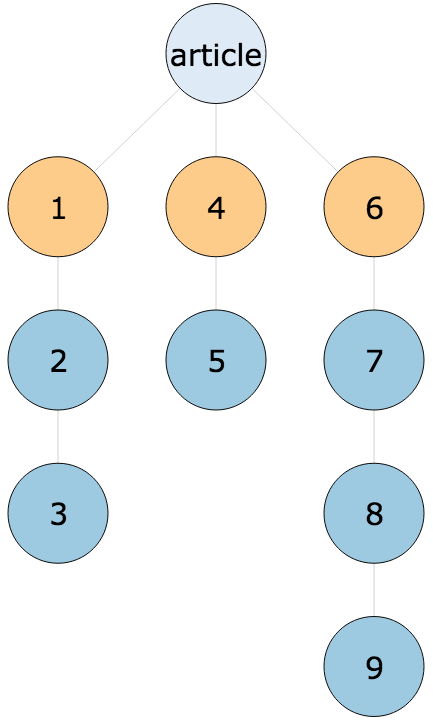
\includegraphics[width=0.36\textwidth]{images/datasets/sequential_structure.png}
  \end{center}
  \caption{The comments 1, 4 and 6 are top-level comments, all others are replies.}
\end{wrapfigure}

The online web service provider Yahoo operates a news outlet called Yahoo News\footnote{\url{https://news.yahoo.com}}. They do not produce own news stories but feature the stories of other outlets. They cover a broad range of topic from politics, to sports to lifestyle. Readers can comment under the articles and there are two types of comments.
There are \textit{top-level comments} that are directly sequential under the article and \textit{replies} that follow-up on a top-level comment.
Unlike other web services such as Reddit, there is no tree-structure. There is only a sequential flow of top-level comments under the article. And each top-level comment can have a sequential flow of replies. The authors used the term \textit{sub-dialogue} to describe a top-level comment including all its replies.

Napoles et al. collected over 230k comments from over 34k sub-dialogues under over 2.8k articles. The comments were written between August 2014 to May 2016. For a subset of 9160 comments, they employed annotators to label them. The dataset contains the comment identifier for training, validation, and test set in a ratio of about $87\%$, $6\%$ and $6\%$. It is worth mentioning that there are different groups of annotators for training and validation, and the test set. The authors used crowd workers to annotate the comments from the training and validation set. Different `Expert annotators' were employed to code the test set.
The comments were annotated on the sub-dialogue level as well as the comment level.
In this master's thesis, we focus on the comment level and therefore neglect the sub-dialogue annotations.
Originally, the authors annotated for over 15 categories but refined to nine categories afterwards. We quote from the annotator notes\footnote{\url{https://github.com/cnap/ynacc/blob/master/rater-guidelines.pdf}} to describe the different classes:
\begin{description}
    \item \item [Persuasive] ``This is an opinion based on whether you think the user means to be persuasive and how persuasive they seem to be. Generally, the commenter incorporates new information or a personal story, or uses specific language in attempt to convince other users of his or her point. In order for a comment to have true persuasiveness, they must present a well-reasoned argument.''
    \item [Audience] ``Choose whether the comment is meant to be 1) a reply to a specific commenter; 2) broadcast message/general audience; [..] Please note that a top-level comment with ALWAYS be a broadcast message with a general audience, by nature of being a top-level comment.''
	\item [Agreement] ``Agreement with other commenter: The comment indicates agreement with either another commenter explicitly, meaning, the user is clearly expressing they agree with another person or point of view in the thread. Can occur concurrently with other types of agreement/ disagreement.''
	\item [Informative] ``Informative (Constructive, Productive): This comment furthers the discussion by adding new information. Usually an attempt to be persuasive and convince others of the user's argument. It may be passionate, but it is not dismissive. NOT a personal story. Criteria for informativeness: 1. Mention of historical facts or evidence 2. Mention of statistics and other numbers 3. Quote or paraphrase of public discourse made by a popular figure 4. Mention of events, or `news' 5. Presenting a cogent or logical analysis or argument''
	\item [Mean] ``Mean (Hateful): The comment is intended to be rude, mean, or hateful with no other intent. Be careful to not assign this to comments you personally disagree with. Note that mean, hateful comments/insults can still be on topic with the article or conversation.''
	\item [Controversial] ``Controversial (Outspoken): This comment puts forth a strong opinion in a way that others will certainly strongly disagree with.''
	\item [Disagreement] ``Disagreement with other commenter: The comment indicates disagreement with either [sic] another commenter. Can occur concurrently with other types of agreement/ disagreement.''
	\item [Off-topic] ``Off topic with article: The conversation/contributions have begun to be irrelevant to the article (Also can be thought of as a digression). Each contribution that is off topic to the article once an off-topic conversation has begun should get an `off-topic' flag. Once a digression begins, every contribution within the digression is on topic with that conversation but OFF topic with the article.''
	\item [Sentiment]
		Positive: ``A positive sentiment generally expresses feelings of positive emotion, for example `I love the Yankees! Gunna be a great year.' When users express their opinion on something as being great or good, this is a positive sentiment. Attempts at making jokes or at being funny to `lift the mood' generally have a positive sentiment, unless they are mean-spirited.''
		
		Negative: ``A negative sentiment is more common and indicates the commenter is unhappy for some reason. Usually goes in hand with some complaint about the world or the issue. For example, `Donald Trump sucks. I can't believe he's allowed to be in the public eye.' Additionally, mean or controversial comments are usually coming from a negative emotional place on the part of the commenter. Sarcasm, although funny, is usually used to express discontent or absurdity, is usually negative.''
		
		Neutral: ``A neutral sentiment has no emotion. Usually when a commenter is just stating fact, like `I think the season starts in July, actually.' or `If you water your basil every day, it shouldn't die'.''
		
		Mixed: ``A mixed sentiment is when a user seems to express both positive and negative emotion about something or several things. A good example is when a commenter expresses that they are in agreement with something one commenter said, but also is offended or takes issue by something else. Longer comments that contain many expressions of different emotions are usually `mixed'.''
\end{description}


\begin{figure}[h]
    \centering
    \subfloat[Binary Categories]{{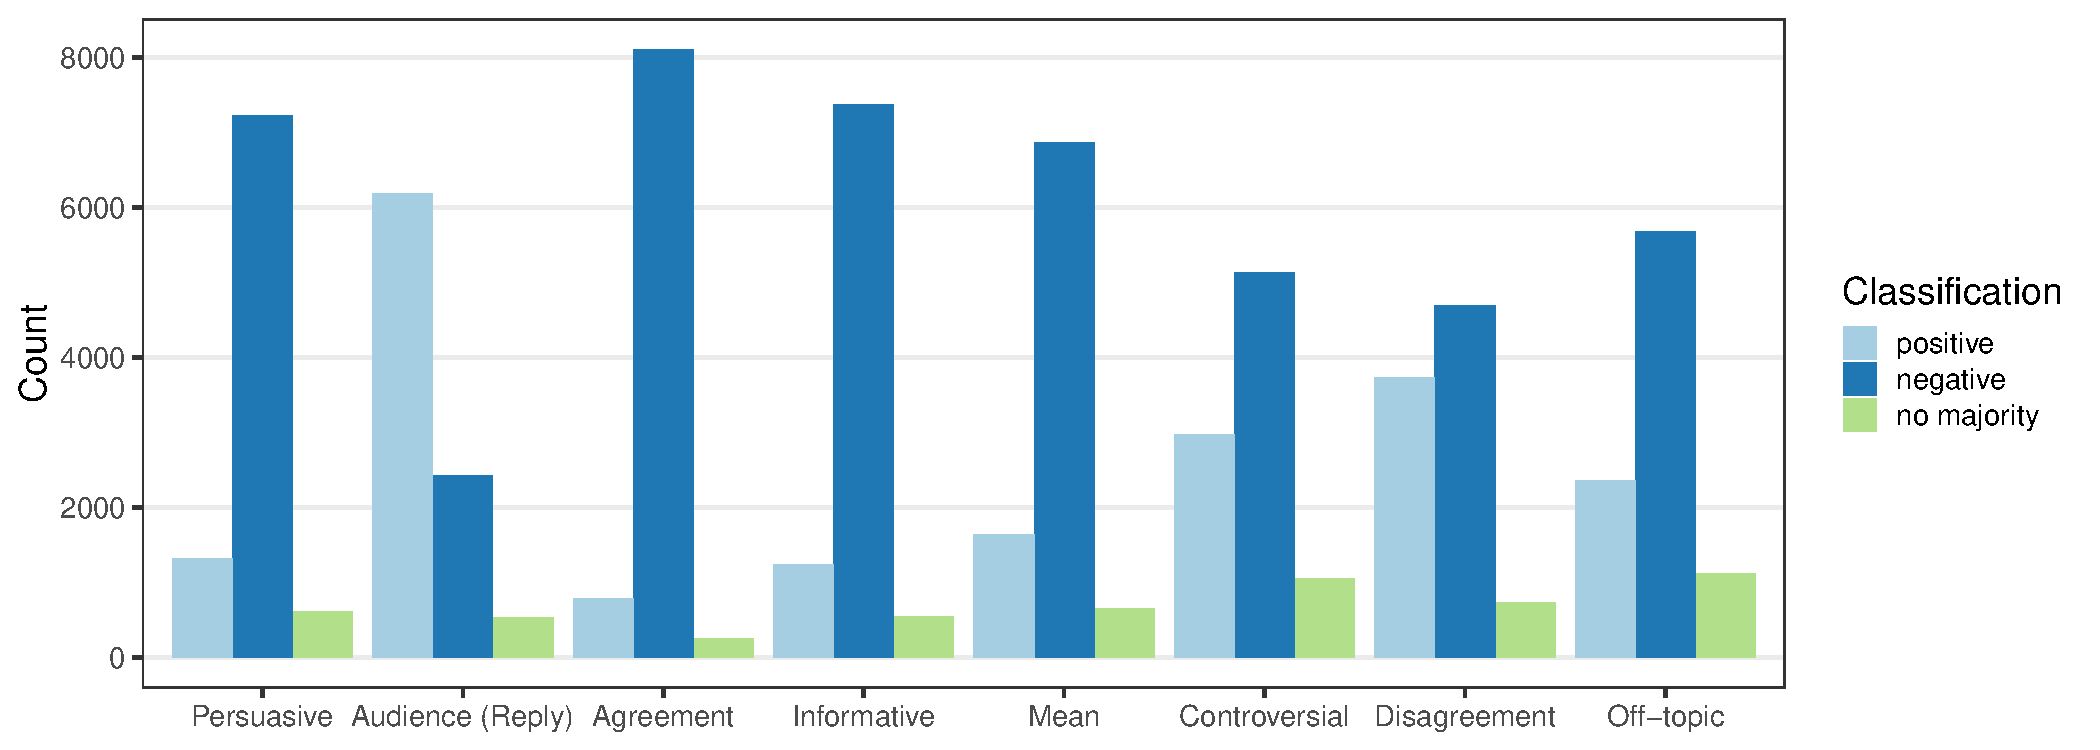
\includegraphics[height=110pt]{graphs/class_distributions/class_dist_ynacc_bin_no_maj} }}
    \subfloat[Sentiment]{{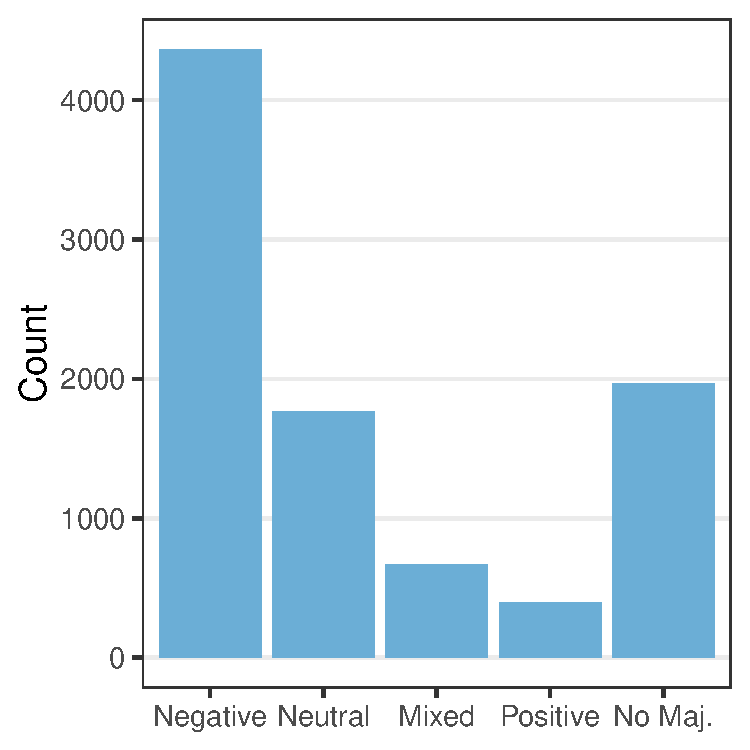
\includegraphics[height=110pt]{graphs/class_distributions/class_dist_ynacc_sentiment_no_maj} }}
    \caption{The distributions for each category where the number of samples without majority vote is present.}
    \label{fig:class_distru_no_maj}
\end{figure}
\begin{figure}[h]
    \centering
    \subfloat[binary categories]{{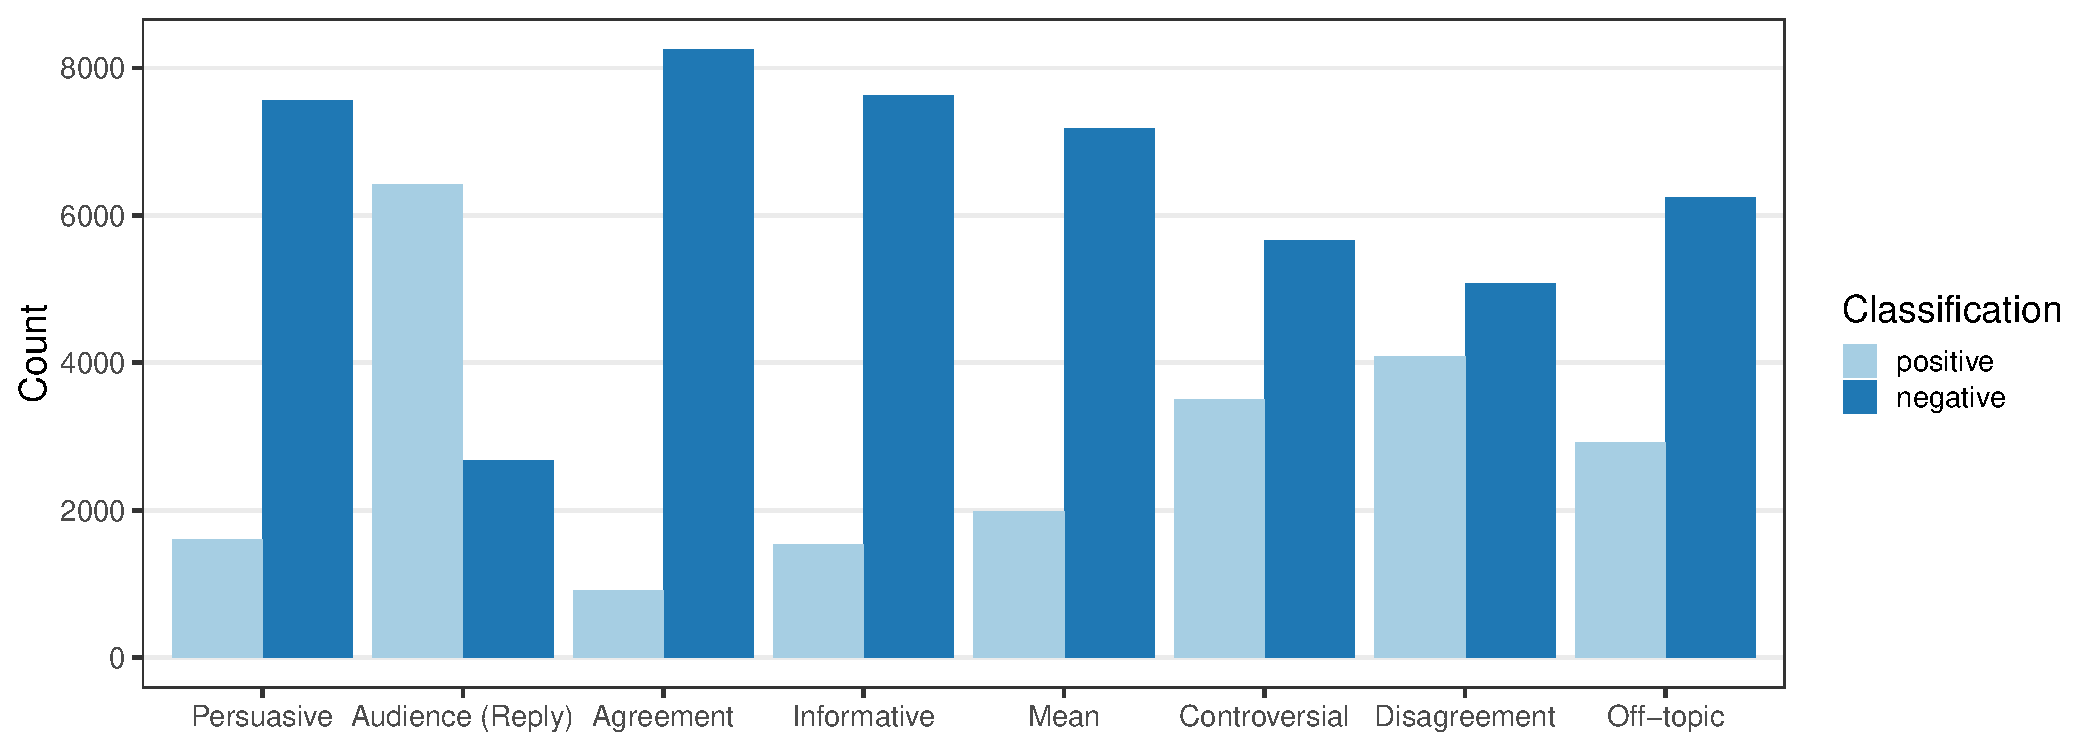
\includegraphics[height=110pt]{graphs/class_distributions/class_dist_ynacc_bin} }}
    \subfloat[Sentiment]{{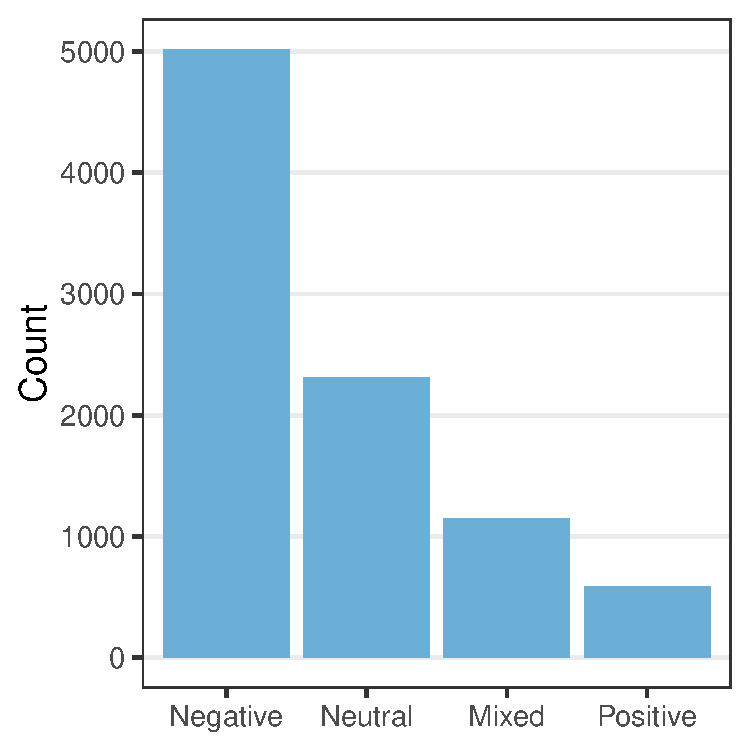
\includegraphics[height=110pt]{graphs/class_distributions/class_dist_ynacc_sentiment} }}
    \caption{The final distributions for each category.}
    \label{fig:class_distru}
\end{figure}

Napoles et al. only publish the raw annotations\footnote{\url{https://webscope.sandbox.yahoo.com/catalog.php?datatype=l&did=83}} for each annotator.
So for using the data for classification, one has to consolidate the annotations to derive a final assessment.
In the authors' follow-up work~\cite{napoles2017automatically}, they choose a majority vote for each sample. If there is no majority for a class, they randomly choose an applicable class, according to the authors' post on GitHub\footnote{\url{https://github.com/cnap/ynacc/issues/2}}. Consequently, to compare results, it is advised to replicate their approach.
In Figure~\ref{fig:class_distru_no_maj} is the number is the number of undecided samples visualized.
The binary categories Controversial and Off-topic have the largest share of un-decided samples.
Over 1000 samples, almost 10\% of the data, are randomly assigned to classes.
While the share for Sentiment is large as well, it is a four-class setup so dissension is more likely.
The random selection is done for each applicable label.
So undecided samples do not get uniformly distributed over the four classes.
In Figure~\ref{fig:class_distru} is the final outcome of this procedure shown.
As it is often the case with real-life data, the distributions are mostly imbalanced.
Agreement is the most imbalanced while Disagreement is almost balanced.

\begin{figure}
    \centering
    \subfloat[unlabeled comments (YC\textsubscript{LM})]{{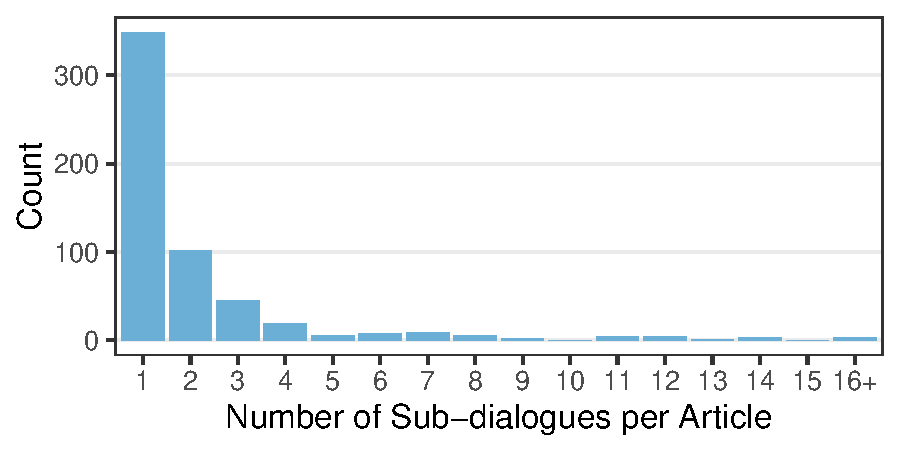
\includegraphics[width=0.5\textwidth]{graphs/eda/threads_per_article_cl} }}
    \subfloat[annotated comments (YC\textsubscript{CL})]{{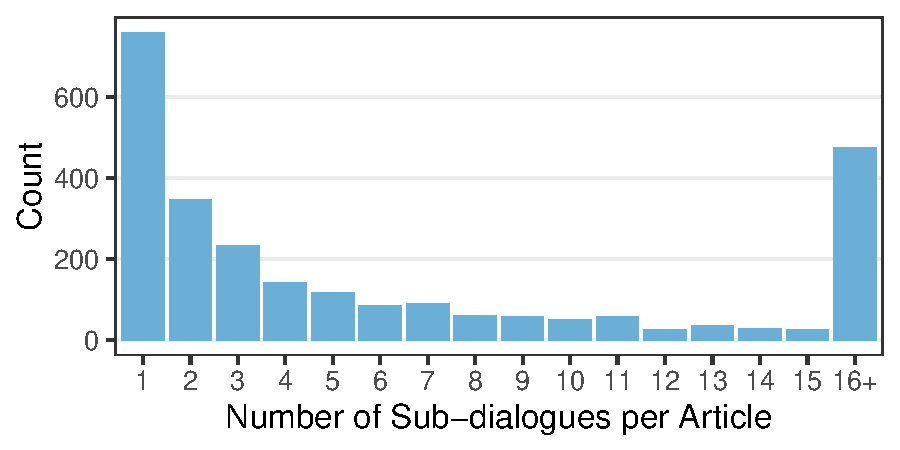
\includegraphics[width=0.5\textwidth]{graphs/eda/threads_per_article_lm} }}
    \caption{The number of sub-dialogues per article.}
    \label{fig:threads_per_article}
\end{figure}

In addition to the annotated comments, the YNACC contains a large number of unlabeled comments.
After cleaning the data, as it will be described in Subsection~\ref{subsec:ynacc_data_cleaning}, about 238k unique comments remain.
As we will train a language model which does not require annotations, the unlabeled is also part of this work.
In the following, we provide several graphs comparing the characteristics of unlabeled comment set, we denote as YC\textsubscript{LM} with the portion of labelled training data YC\textsubscript{CL}.
In Figure~\ref{fig:threads_per_article} is the number of sub-dialogues per article are shown.
There is a stark difference between the two sets of comments with a lot more articles having only one annotated sub-dialogue. In Figure~\ref{fig:replies_per_thread} is the the frequency of number of replies for each top-level comments.
There are only a fews comments in the columns 0--2.
This is most likely the reason for some sampling. In Figure~\ref{fig:threads_per_article} the frequency of comments per rank is displayed. Here ranks refers to the distance to the parent comment. The top-level comments have a rank of 0 and no parent comments. While the information is the same in both graphs, Figure~\ref{fig:threads_per_article} gives a better feeling of how large the share of comments on the early ranks is. Finally, to get a better sense of YC\textsubscript{LM}, we list the 30 most frequent tokens in Figure~\ref{fig:word_freq}, excluding stop words and tokens with a length of three or less.
In Figure~\ref{fig:len_com} is the number of tokens for the comments. This allows to truncate the comments to abolish outliers. And since word based approaches rely on fixed vocabulary, we plot the share of all token covered by choosing only N most frequent tokens in Figure~\ref{fig:vocab_size}.

\begin{figure}
    \centering
    \subfloat[Unlabeled comments (YC\textsubscript{LM}).]{{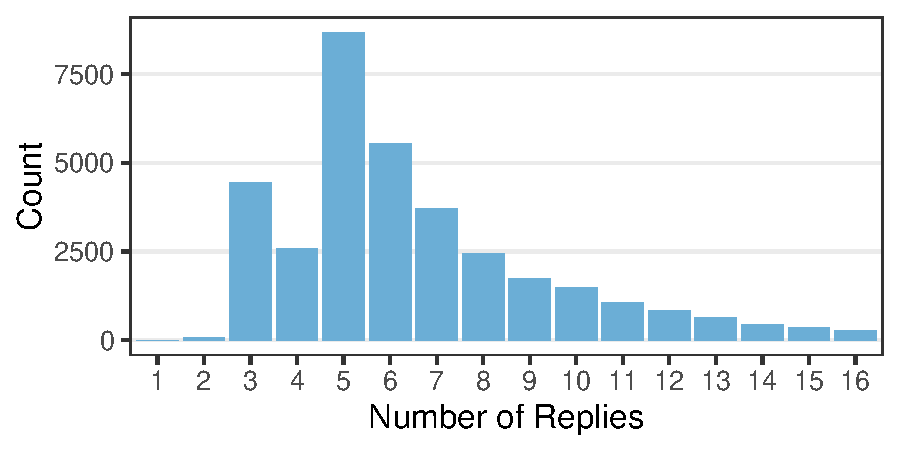
\includegraphics[width=0.5\textwidth]{graphs/eda/lm_num_replies} }}
    \subfloat[Annotated comments (YC\textsubscript{CL}).]{{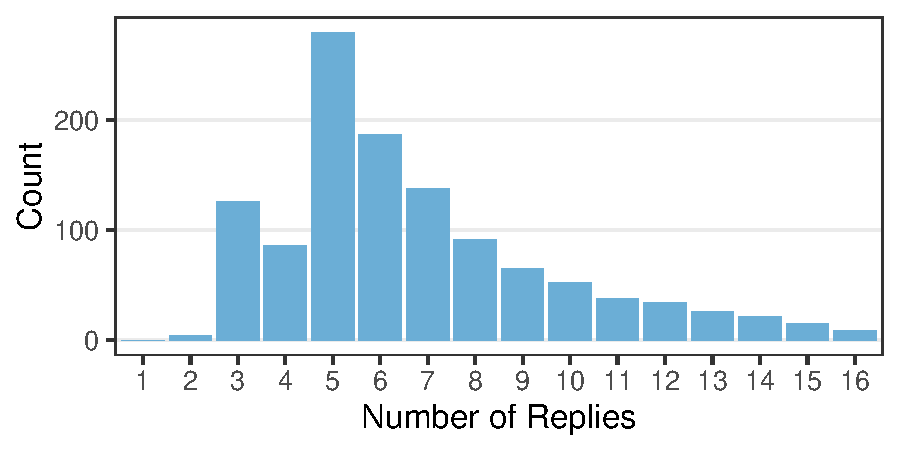
\includegraphics[width=0.5\textwidth]{graphs/eda/cl_num_replies} }}
    \caption{Frequency of number of replies for each top-level comment.}
    \label{fig:replies_per_thread}
\end{figure}

\begin{figure}
    \centering
    \subfloat[Unlabeled comments (YC\textsubscript{LM}).]{{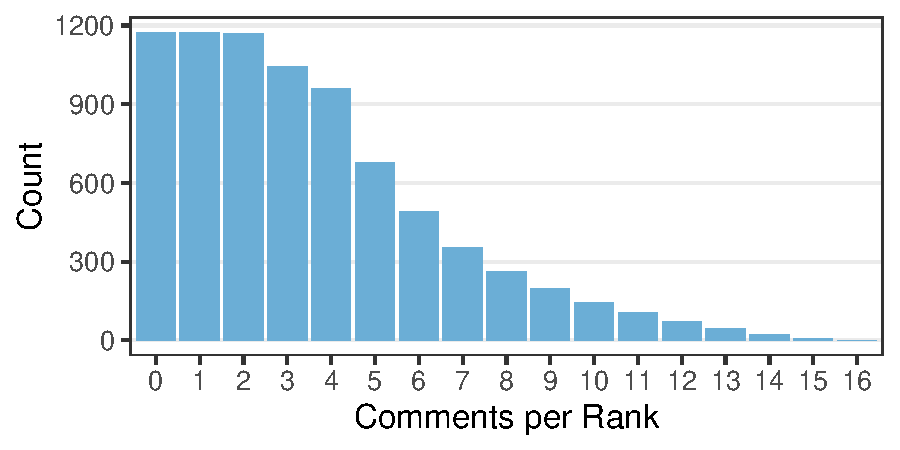
\includegraphics[width=0.5\textwidth]{graphs/eda/comments_per_rank_cl} }}
    \subfloat[Annotated comments (YC\textsubscript{CL}).]{{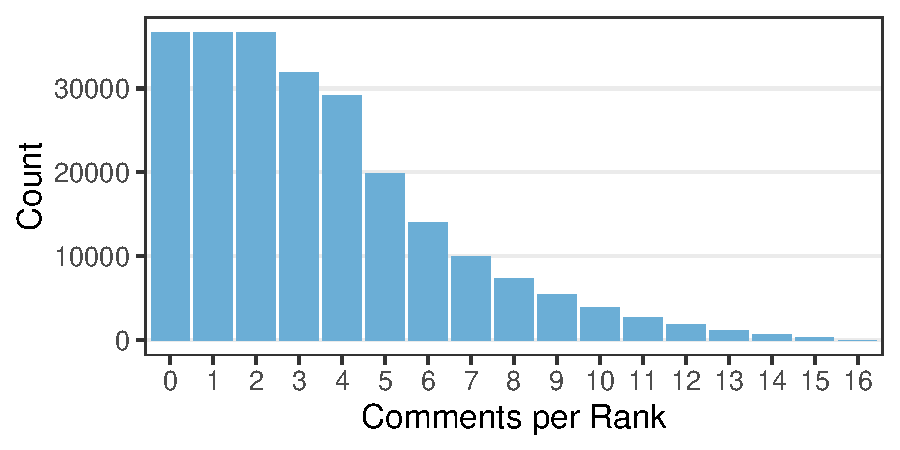
\includegraphics[width=0.5\textwidth]{graphs/eda/comments_per_rank_lm} }}
    \caption{Frequency of comments per rank.}
    \label{fig:comments_per_rank}
\end{figure}

\begin{figure}
    \centering
    \subfloat[Number of tokens in a comment, truncated at 300.\label{fig:len_com}]{{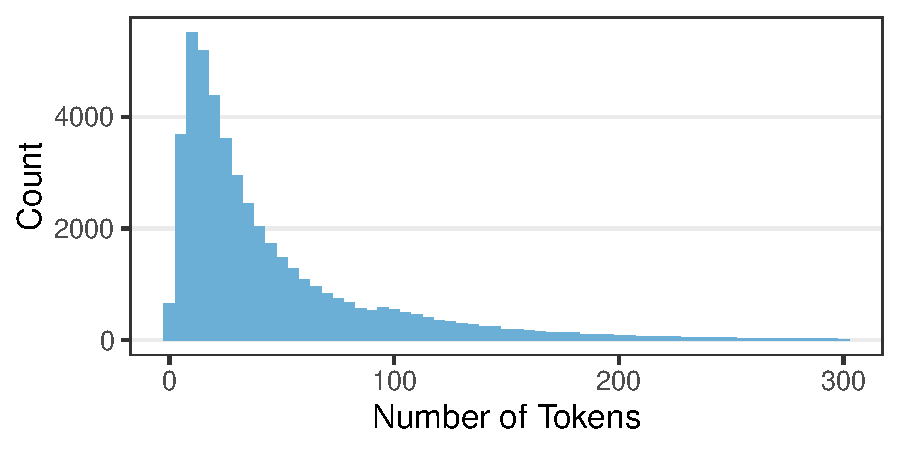
\includegraphics[width=0.5\textwidth]{graphs/eda/comment_length} }}
    \subfloat[Share of text covered by fixed vocabulary size.\label{fig:vocab_size}]{{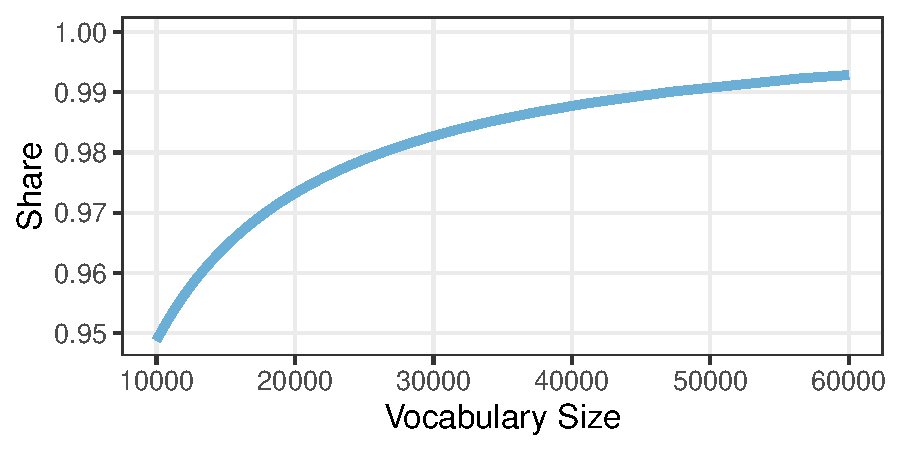
\includegraphics[width=0.5\textwidth]{graphs/eda/max_vocab} }}
    \caption{Text analysis of YC\textsubscript{LM}.}
    \label{fig:word_based_anal}
\end{figure}

Besides the text, each comment has the number of up-votes, timestamp, parent comment id (if it is a reply), and the article's headline and URL. The article text is not part of the datasets. We were able to crawl about 80 percent of the article  texts to not limit ourselves to the headline. Since a lot of articles are offline, we resorted to the Internet Archive's Wayback Machine\footnote{\url{https://archive.org/web/}} to fetch them.
The data of the articles were extracted using the Python package Newspaper3k\footnote{\url{https://github.com/codelucas/newspaper}}.
Information about the comment's author is also not part of the datasets.
In addition, all mentions of usernames were replaced by the token \textit{@username}.

%\vspace{-25pt} %no idea if useful
\begin{wrapfigure}[16]{r}[-5pt]{0.4\textwidth}
  \begin{center}
    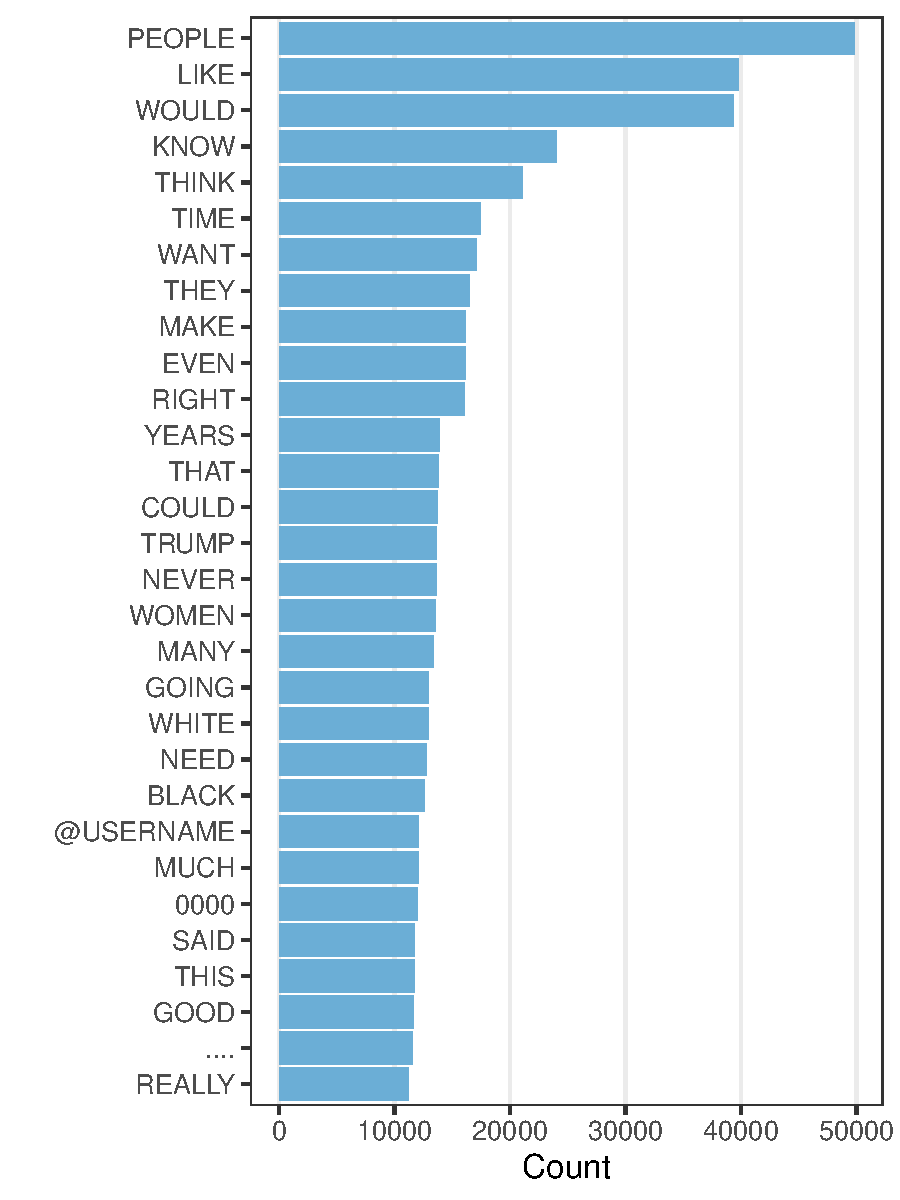
\includegraphics[width=0.36\textwidth]{graphs/eda/word_freq}
  \end{center}
  \caption{The 30 most frequent tokens in YNACC.}
  \label{fig:word_freq}
\end{wrapfigure}

\subsection{Data Cleaning}
\label{subsec:ynacc_data_cleaning}

The provided data is `dirty'.
There are duplicated rows as well as corrupted text encodings.
In addition, due to the nature of user-generated text, there are other issues, e.g., different forms of quotation marks. So first, the text is cleaned with the Python package \textit{clean-text}\footnote{\url{https://github.com/jfilter/clean-text}. The package was developed over the course of this master's thesis and borrows code from another Python package textacy: \url{https://github.com/chartbeat-labs/textacy}.} in the following way: whitespaces are normalized but (single) newlines are kept, UTF8 encoding issues are fixed, the text is transliterated to ASCII and the casing is kept. All digits are replaced by a `0'.
Then, duplicated rows were removed.
First, duplicates based on comment ID and text were deleted.
Second, rows with duplicated ID but different text were cleaned.
This situation occurred because some characters such as quotations marks were stripped from some rows.
So in the case of duplicated IDs but different text, we chose the sample with the longest text.

\subsection{Reported Values}
\label{subsec:ynacc_reported}

Napoles et al.~\cite{napoles2017automatically} report in the accompanying publication results for the classification of individual comments.
Even though the focus are predictions on thread-level.
Unfortunately, it is unclear which kind of metrics they used and they also did not respond to our email.
They only write that they use precision, recall and $\text{F}_{1}$ score.
We report their values in Table~\ref{tab:ynacc_reported} and try to convert their values into our metric of choice: Cohen's Kappa.
We gave background information about metrics for classification and shortcomings of the $\text{F}_{1}$ score in Section~\ref{sec:metrics}.

\begin{table}
\nprounddigits{3}
\small
\centering
\caption{Reported Results on YNACC and their conversation into Cohen's Kappa.}
\label{tab:ynacc_reported}
\begin{tabular}{l l l l  n{1}{3} n{1}{3} n{1}{3} n{1}{3} n{1}{3} n{1}{3}}
\toprule
\multicolumn{1}{l}{} & \multicolumn{3}{c}{Reported} & \multicolumn{6}{c}{Calculated} \\
\cmidrule(r){2-4}
\cmidrule(r){5-10}
\multicolumn{4}{l}{} & \multicolumn{3}{c}{Presence = Positive} & \multicolumn{3}{c}{Absence = Positive} \\
%\cmidrule(r){2-4}
\cmidrule(r){5-7}
\cmidrule(r){8-10}
\multicolumn{1}{l}{Category} & \multicolumn{1}{l}{Precision} & \multicolumn{1}{l}{Recall} & \multicolumn{1}{l}{F\textsubscript{1 binary}} & \multicolumn{1}{l}{F\textsubscript{1 micro}} & {F\textsubscript{1 macro}} & {Kappa} & \multicolumn{1}{l}{F\textsubscript{1 micro}} & {F\textsubscript{1 macro}} & {Kappa}  \\
\midrule
Persuasive & $0.81$ & $0.84$ & $0.91$ & 0.9468267581475128 & 0.8947953594234788 & 0.7896017415802279 & 0.7013422818791947 & 0.41222879684418146 & -0.17343597911689246 \\
Audience & $0.80$ & $0.99$ & $0.88$ & 0.8296041308089501 & 0.7808674781416081 & 0.5751386806319849 & 0.9122203098106713 & 0.9071317756569979 & 0.8155406288713061 \\
Agreement & $0.69$ & $0.85$ & $0.76$ & 0.9382504288164666 & 0.8638274680784803 & 0.7281065395377759 & 0.6151685393258427 & 0.38086956521739135 & -0.1841456752655537 \\
Informative  & $0.76$ & $0.74$ & $0.75$ & 0.9193825042881647 & 0.8516081515057974 & 0.7032307675645233 & 0.5990016638935108 & 0.3746097814776275 & -0.249868404021228 \\
Mean & $0.74$ & $0.78$ & $0.75$ & 0.8970840480274442 & 0.6798847989117535 & 0.6927536231884058 & 0.6112054329371817 & 0.37934668071654365 & -0.23774696484450275 \\
Controversial & $0.67$ & $0.64$ & $0.65$ & 0.5746140651801029 & 0.5630107838870352 & 0.15794623305222943 & 0.5420240137221269 & 0.487601591894374 & -0.023822834930511405 \\
Disagreement & $0.60$ & $0.68$ & $0.64$ & 0.6878216123499142 & 0.6816769068305093 & 0.36530363210030137 & 0.5385934819897084 & 0.5010102167113708 & 0.008985838773072685 \\
Off-topic & $0.62$ & $0.67$ & $0.61$ & 0.4922813036020583 & 0.3790016121602948 & -0.23743689765947673 & 0.7684391080617495 & 0.7368473845227945 & 0.47409040793825796 \\
%\midrule
Sentiment & 0.44 & 0.46 & 0.43 \\
\bottomrule
\end{tabular}
\end{table}

It seems like the authors did not average the metrics but only chose one class as the positive one. There are several indications for this. Micro-averaged values are ruled out because precision, recall and $\text{F}_{1}$ would be identical.
For macro-averaging, the values would be extremely strong, i.e., with a recall of 0.99 for the category Audience. They could have used weighted average but this is rather uncommon so they would have mentioned it in the paper. So it is more probable that the authors refrained from averaging.
To distinguish this from averaged score, we refer to it as F\textsubscript{1 binary}  in Table~\ref{tab:ynacc_reported}.
The strong performance of recall for Audience may be due to choose the majority class the positives class\footnote{The F\textsubscript{1} differs depending on what class is the positive and what is the negative class.}.
This shows that $\text{F}_{1}$ scores do not always yield meaningful evaluation. As a consequence, we convert the results into Cohen's Kappa. To do so, we reconstruct $fp$, $tp$, $tn$, and $fn$\footnote{These are the acronyms for false positives, true positives, true negatives, false negatives respectively.}. But since the binary metrics are always in respect to one class, that we do not know, we have calculate them for both situations.
So the table consists of values if the original results came from the presence and the absence of a specific class.
We can to the conversation because we have four unknowns and four equations. We have precision and recall.
And since we know the distributions of the classes (because we have the samples), we can derive two additional equations:

\begin{align*}
    class_0 &= tp+fn & class_1 &= fp+tn\\
\end{align*}

This enables us to solve for the four unknown variables. With them, we can calculate a different metric, in this case Kohen's Kappa. But we only do this for the eight binary classes.
The category Sentiment has four classes and thus we cannot reconstruct the original values.
In the original paper, the authors reveal that the results for the categories Informative and Controversial are below a simple ridge regression baseline.

We will continue to discuss the values in the evaluation Section~\ref{sec:exp_ynacc_results} to set our contribution into perspective.

\subsection{Discussion}

There are several issues with the YNACC dataset:
\begin{itemize}
	\item It is unclear what metric was used for the reported values. Since the authors did not reply to our email, we and others researchers can only speculate. This makes it hard to compare results and sets new inventions into perspective.
    \item For the consolidation of annotations, the authors decided to randomly assign samples to classes when there is no majority among the annotators. This adds unnecessary noise. It is most likely better to fully remove the samples from dataset.
    \item The authors did not provide the consolidated assignment for the samples. Therefore, it is not fully clear, how they derived the values. For instance, there are classes marked as `NA'. It is unclear whether they were removed or kept.
    \item Two different groups of people annotated the data. One group annotated training and validation and the other group, ``expert annotators'' the test set. It is true, that the test set is used to evaluate the performance of a model in the wild. However, then the test set cannot be used to asses the performance of the model. A model can only learn what is has been taught.
\end{itemize}

Nevertheless, it is still the largest corpus of publicly available news comments. We follow the setup of the original paper, including the random assignments to compare our results.

\section{One Million Posts Corpus}
\label{sec:ompc_ds}

The One Million Posts Corpus\footnote{\url{https://ofai.github.io/million-post-corpus/}} (OMPC) is a dataset consisting of German comments from the Austrian newspaper \textit{DerStandard}\footnote{\url{https://derstandard.at/}}.
The dataset was presented in-depth in the publication by its creators Schabus et al.~\cite{Schabus:2017:OMP:3077136.3080711} and thus we only give a brief overview.

\begin{figure}
  \begin{center}
    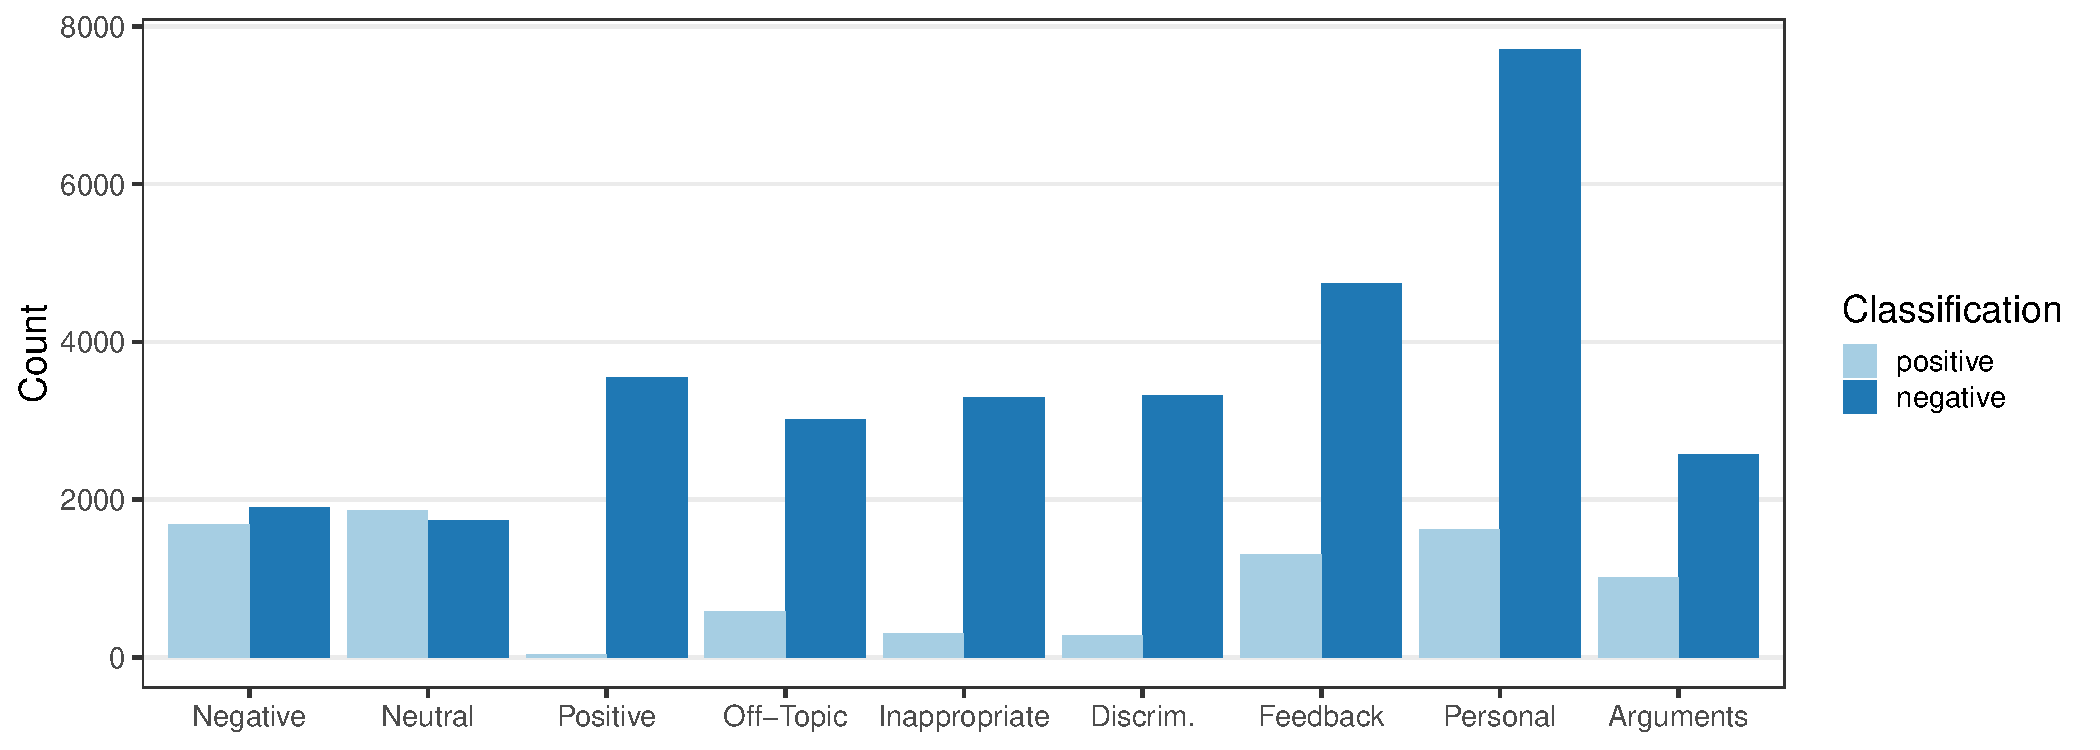
\includegraphics[width=\textwidth]{graphs/class_distributions/class_dist_ompc_bin}
  \end{center}
	\caption{The distributions of classes in OMPC are imbalanced. Also the number of samples varies among the categories.}
   \label{fig:data_ompc_distu}
\end{figure}

It contains 1 million unlabeled comments and 11,773 labeled ones from 2015 to 2016. A comment consists of its text, user votings and pseudonymized author ID but also information about the article is included: the article's text, headline, topic, and timestamps. The comments were labeled by professional comment moderators in seven categories.
One category, sentiment, is annotated into three classes. All others are binary classifications. They are presented as follows:
\begin{description}
	\item[Sentiment] The sentiment of a comment for three classes: positive, neutral or negative. For further use, the category is split up into three binary classification setups and denoted as \textit{positive}, \textit{neutral} and \textit{negative}.
	\item[Off-topic] If a comment is out of the article's topic.
	\item[Inappropriate] If inappropriate words were used, i.e., swearwords.
	\item[Discriminating] If a comment is discriminating, i.e., racist.
	\item[Personal] If it includes a personal story.
	\item[Feedback] If feedback is given to the article's author.
	\item[Arguments] If arguments are used in a comment.
\end{description}

The number of samples per class varies as shown in Figure~\ref{fig:data_ompc_distu}. The sampling process was done in an interactive way, driven by annotating moderators.
Moderators chose articles under which certain kind of comments appeared often.
For instance, under articles about refugees are a lot of racists comments. So they chose comments from these articles for the category Discriminating. This resulted in a strong bias in the data and thus the annotated data were not sampled representatively. As a consequence, not all comments were assigned with the same class (as the different number for each category indicates). In the publication, the authors provide feature-based as well as neural models results as baselines. They will be presented in Section~\ref{sec:ompc_results} to compare them with our experiment results.

\section{Ethical Considerations}

In this section, the creation of the news comments datasets is reflected critically.

A major problem is the fact, that commentators did not consent for being part of the dataset. Their comments get taken out of the context of the newspaper website in which they originally created them. Then it gets added into the dataset that explicitly invites other people to use it (for research or other purposes). The commentators who contributed to the dataset are most probable not even aware of it. ``Recognize that privacy is more than a binary value'' is one of the ``Ten simple rules for responsible big data research'' that a consortium of 13 researches and philosophers~\cite{DBLP:journals/ploscb/ZookBb0KGGH0MNN17} postulated.
Even though the comment is publicly visible on the newspaper's website, does not give computer scientist do not the right to do everything they desire.
In a research context, when working with user-generated content the same research ethics should apply that exists for social scientists or in the medical domain. One guiding principle is that research participants should consent to being part of experiments. This principle is the result of the discussion after crimes against humanity were done in the name of research during the German National Socialism\footnote{The Nuremberg~Code lists ten rules for human experiments in the aftermath of the Nuremberg trials in 1947. \url{https://en.wikipedia.org/wiki/Nuremberg_Code}}. For future datasets, comments should only be considers if the authors actively agrees to take part in research dataset.
At least information about the comment's author are not in the datasets.
The creators of YNACC fully removed user information whereas the ones for OMPC only created pseudonymized user IDs.


\chapter{Classification of News Comments}
\label{ch:approach}

Our contribution is two-fold: First, we present a preprocessing technique to capture the conversation of a comment for classification.
Second, we adapt ULMFIT for German by training a German language model and publish it for further usage.

\section{Conversation-aware Classification of News Comments}
To exploit the sequential structure of news comment, we propose the preprocessing technique \textit{Prepend Previous} for language-model-based text classification.
News comments appear as part of a conversation where the news article acts as conversation starter.
Only considering each comment in isolation makes it hard to capture its true meaning.
Prepend Previous helps to overcome this restriction.
We prepend previous comments or parts of the article to each comment.
This is similar to the idea of Kochkina et al.~\cite{kochkina2017turing} for Branch-LSTM.
But they use use only word embeddings to represent text.
We use a recent way of using language models for representing text.
And since modern language models can capture dependencies over long distances, the content of a comment can be put into the context of the whole conversation.

\begin{figure}
    \centering
    \subfloat[<t><c>\textbf{1}</c><c>\textbf{2}</c><c>\textbf{3}</c></t>]{{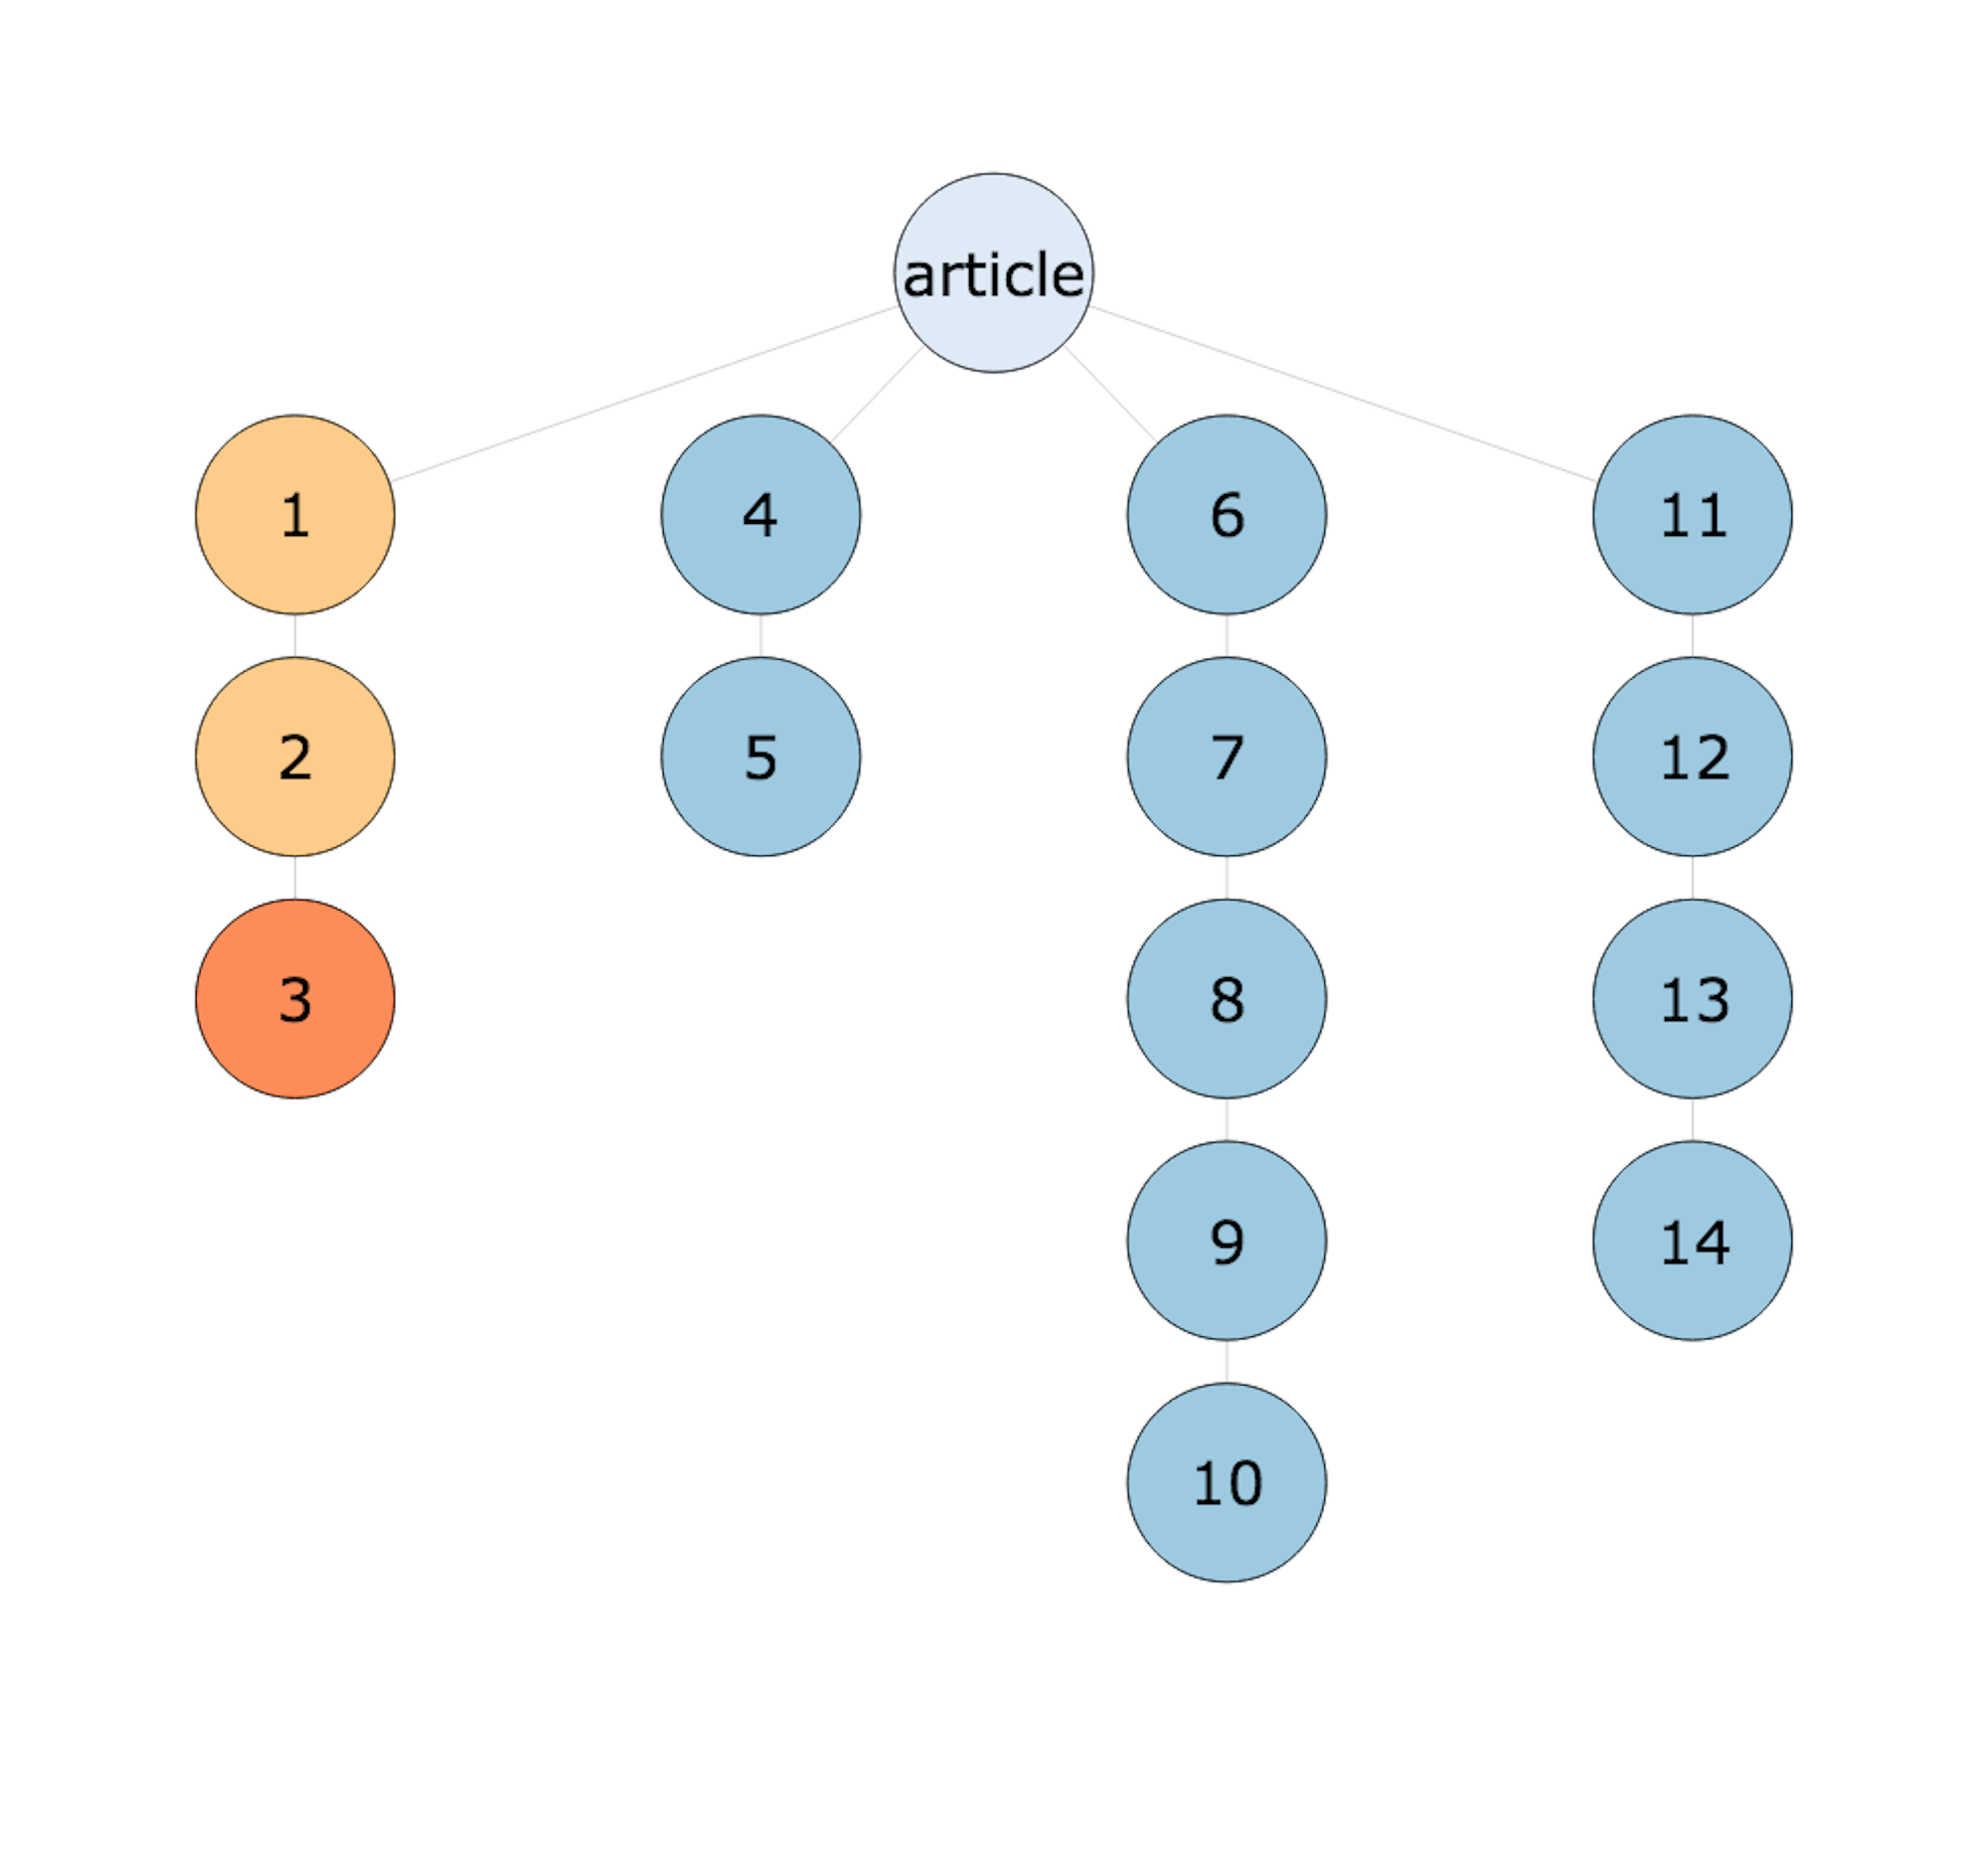
\includegraphics[width=0.5\textwidth]{images/approach/3.png} }}
    \subfloat[<t><c>\textbf{6}</c><c>\textbf{7}</c><c>\textbf{8}</c><c>\textbf{9}</c></t>]{{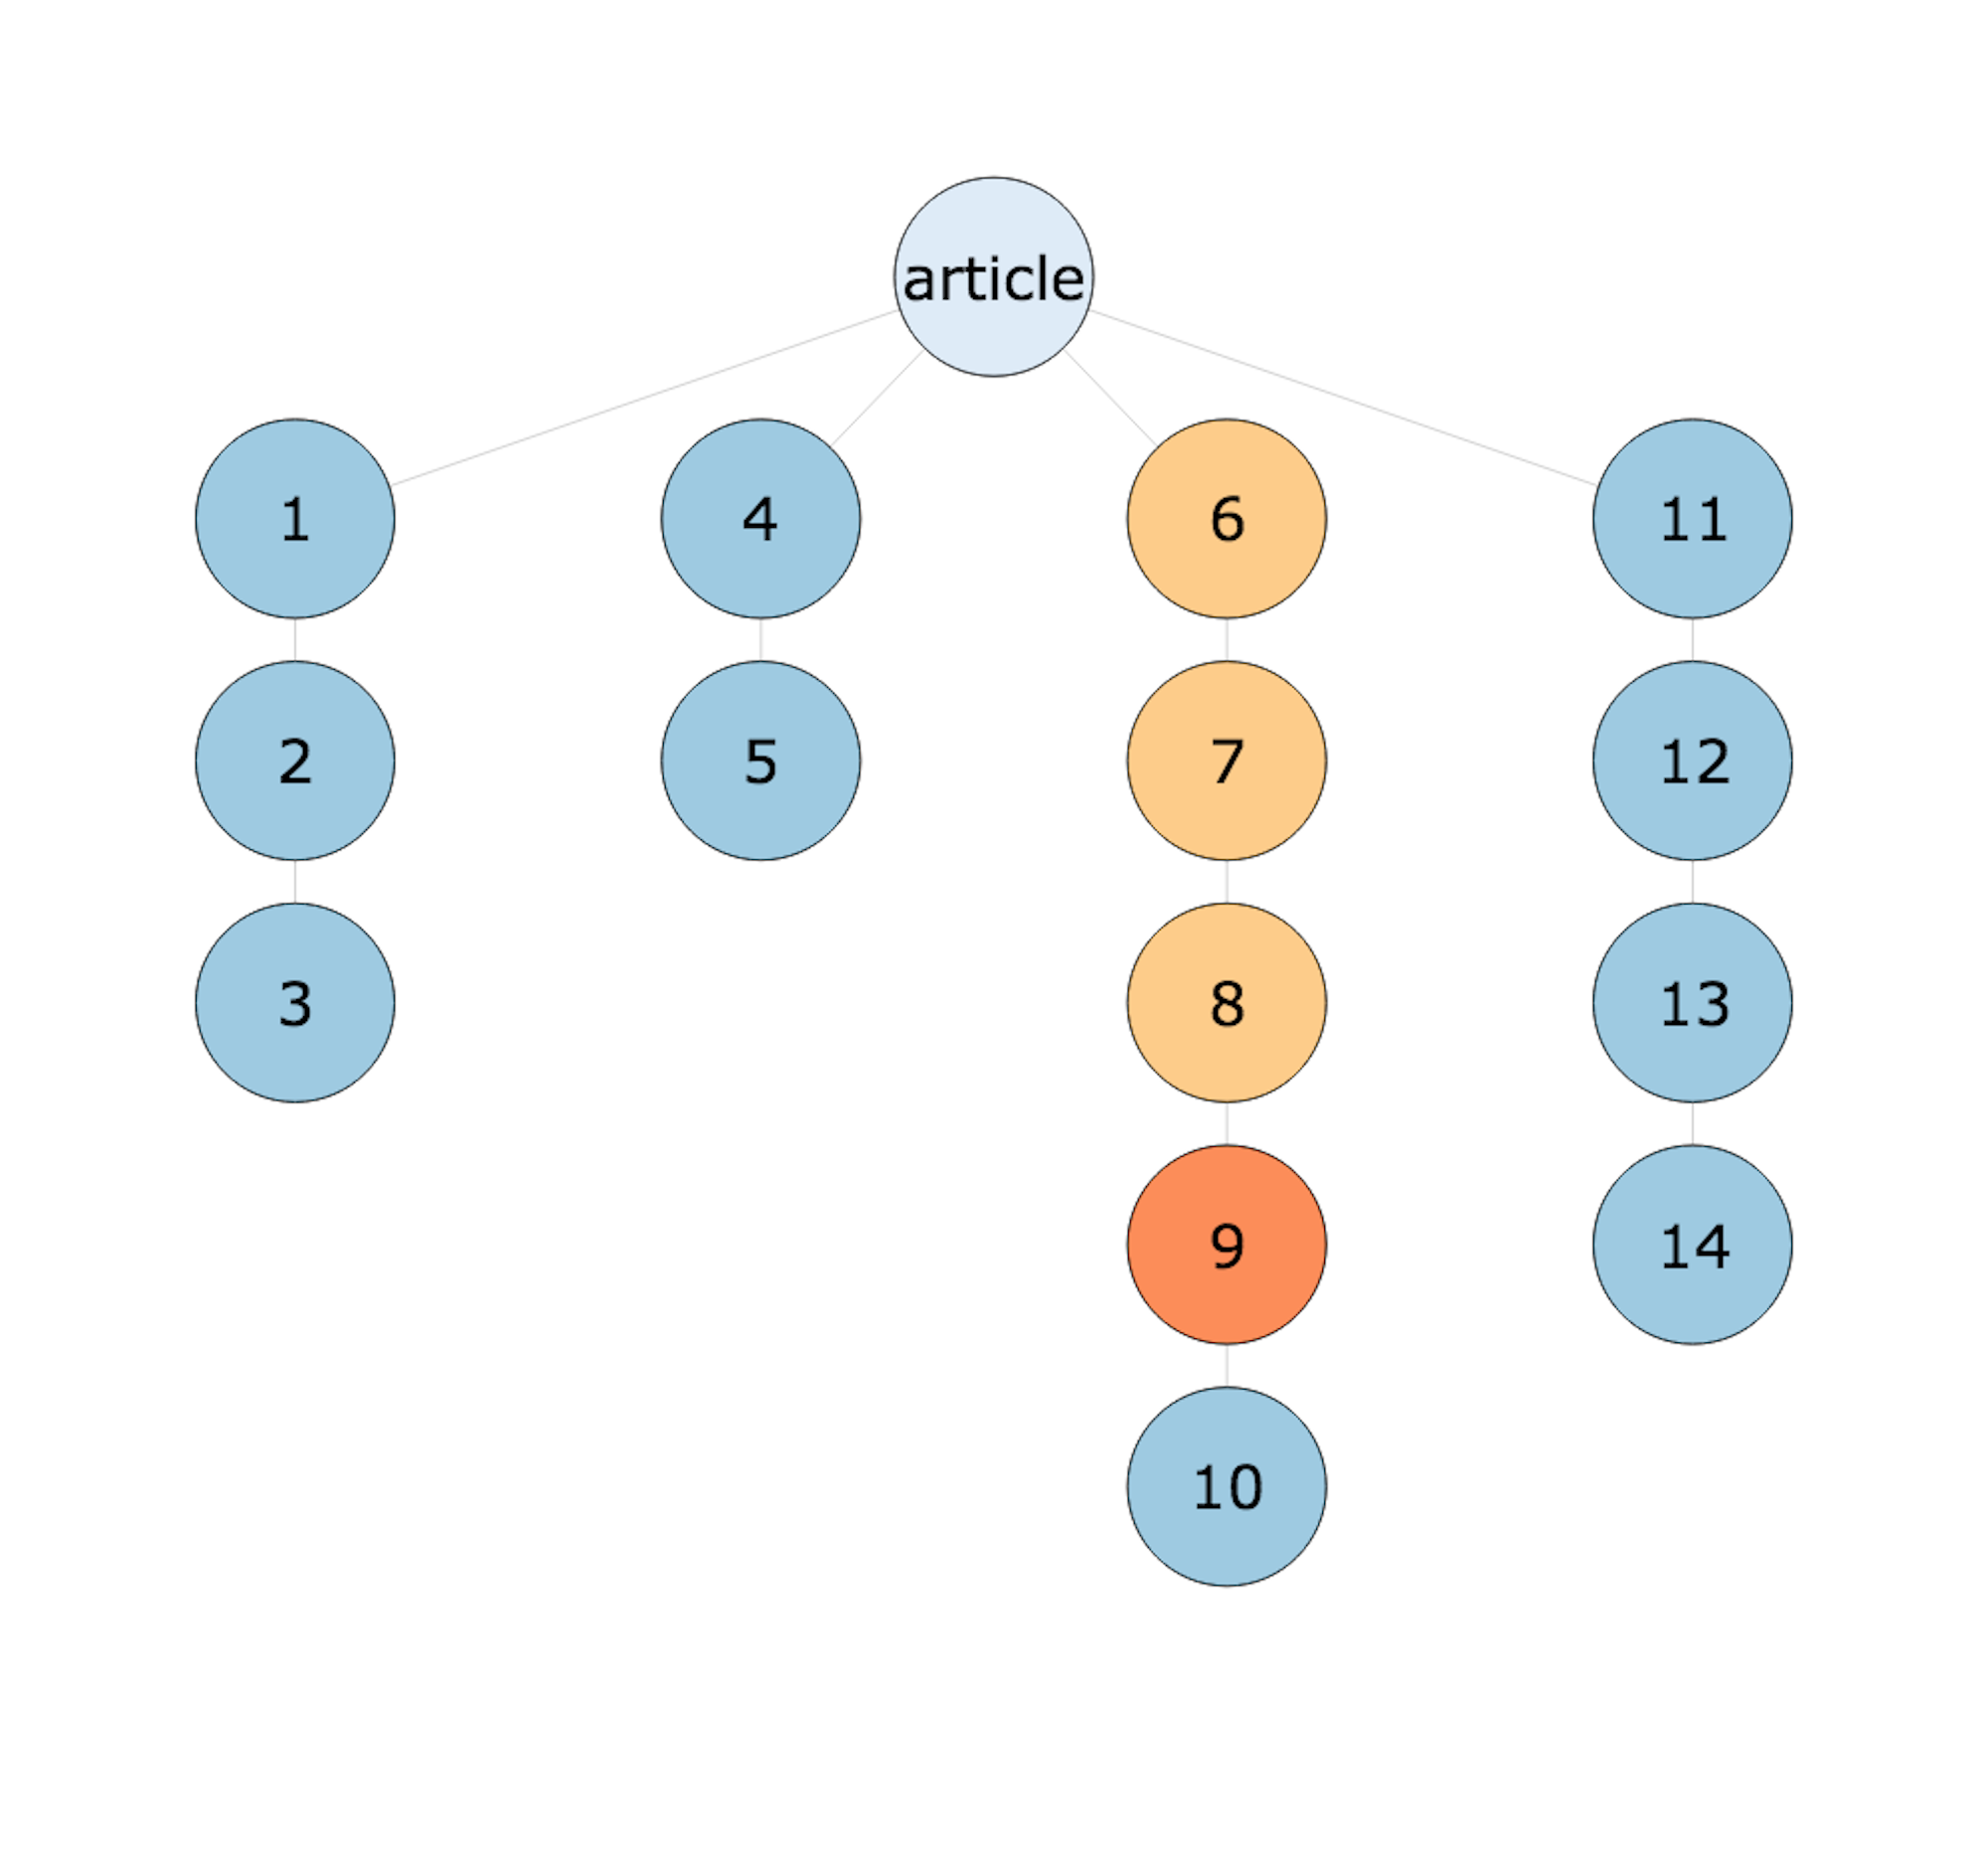
\includegraphics[width=0.5\textwidth]{images/approach/9.png} }}
    \caption{Prepending previous comments at the the example of Comment \textit{3} and Comment \textit{9}. Each comment is encapsulated by the special token (\textit{c}) to mark the start and end of a comment. Also a whole thread is indicated (\textit{t}).}
    \label{fig:approach_1}
\end{figure}

There exist different ways of how comment section appear on the Web.
We focus on sequential discussions where top-level comments appear directly under a news articles and other comments reply to them.
For each reply, we prepend the previous comments.
To separate the comments, we add special tokens between them.
This builds up a long chain of comments.
The comment with the corresponding annotation is always the last comment.
This is how the model can learn that the last comment in the chain is the comment to classify.
The previous comments only give additional information about the conversation.
Figure~\ref{fig:approach_1} illustrates the prepending for two comments. Comment~\textit{3} and Comment~\textit{9} are the samples to which the previous comments are prepended.
For Comment~\textit{3}, the final sequence is <t><c>1</c><c>2</c><c>3</c></t> and the original annotation of Comment~\textit{3} is attached to it.
The <c> and </c> represent the start and the end of comment respectively. Likewise <t> and </t> represent the start and the end of a discussion threads (or sub-dialogue).
To accomplish this, one has to iterate over all comments. % O(n)
Then for each comment, one has to gather all comments that are on the way to the parent node up to the root note -- the news article. %O(n)
This results in a complexity of $\mathcal{O}(n^2)$ for the algorithm.%see above: it's O(n^2), isn't it?

\newpage
In addition, the article's text and headline can be prepended to top-level comments.
There are some variations on how and when top-level comments are enriched.
First, there it is up to debate what kind of information about the article is given the model.
The article comprises headline, abstract, and the whole text.
Also some meta-information such as topic or date of publication are provided.
Second, it has to be decided whether to always add information about an article or only top-level comments.
To illustrate this with an example of the already mentioned Comment~\textit{3}, one could add information before the first comment like so: <t>article<c>1</c><c>2</c><c>3</c></t>.
This has one disadvantage.
Since multiples comments belong to one article, possibly thousands of comments, the article is duplicated in all the training samples.
This may lead to overfitting on the article information such as the title.
So the other idea is to not add article's information to Comment~\textit{3} and only to top-level comments.
For Comment ~\textit{1}, this results in following encoding: <t>article<c>1</c></t>.
The top-level comments do not have any previous comment so no comments can be prepended.
Without article information, there would not be any improvement over conversation-agnostic models for them.

With these adaption, there are potential problems.
Threads with a lot of comments result in duplication of some comments that appear early on in the discussion.
However, in practice internal memory is limited so the samples have to be truncated anyhow.
So here it is important to only truncate from the back to prevent losing valuable information of the last comment (with the annotation).
So for example only choose the last 1000 tokens of a comment chain.
But when cutting the chain on a token basis, it is likely that comments gets cut right in the middle.
This is why there are tokens to indicate the start and end of a comment.
The model is aware that the beginning of a chain is only a remainder of a previous comment.
This way of truncating on a token basis is superior to truncate on a comment basis.
One could think to only consider the previous N comments.
This would as well keep the length of each sample reasonable.
But comments vary in length (see Figure~\ref{fig:len_com}) and thus the sheer number of comments is not a guarantor for information.
The general idea to give as much information as possible to the model and let it decide which information is useful and which not.

So far, we only considered the sequential structure of news comment. Unlike with discussions on social media on Reddit or Twitter, there is often no nesting of replies. \textit{Prepend Previous} focuses on these sequential forms of discussions.
However, it can easily be adapted to to work for tree-like discussion structures.
Again, one has to iterate over all comments and go up the tree until the root.
This is visualized in Figure~\ref{fig:appr_tree_pp}.
In this case, the comments chains may have to be truncated more aggressively since it can happen that a comment appear in various sequences.
Overfitting on those comment is likely when fine-tuning a language model.
However, since there should be no fundamental difference between comments appearing earlier and later in a discussion, the language model should still be able to learn the languages of news comments.
Even if it sees comments appearing early in a discussion tree more often.

\begin{figure}
  \begin{center}
    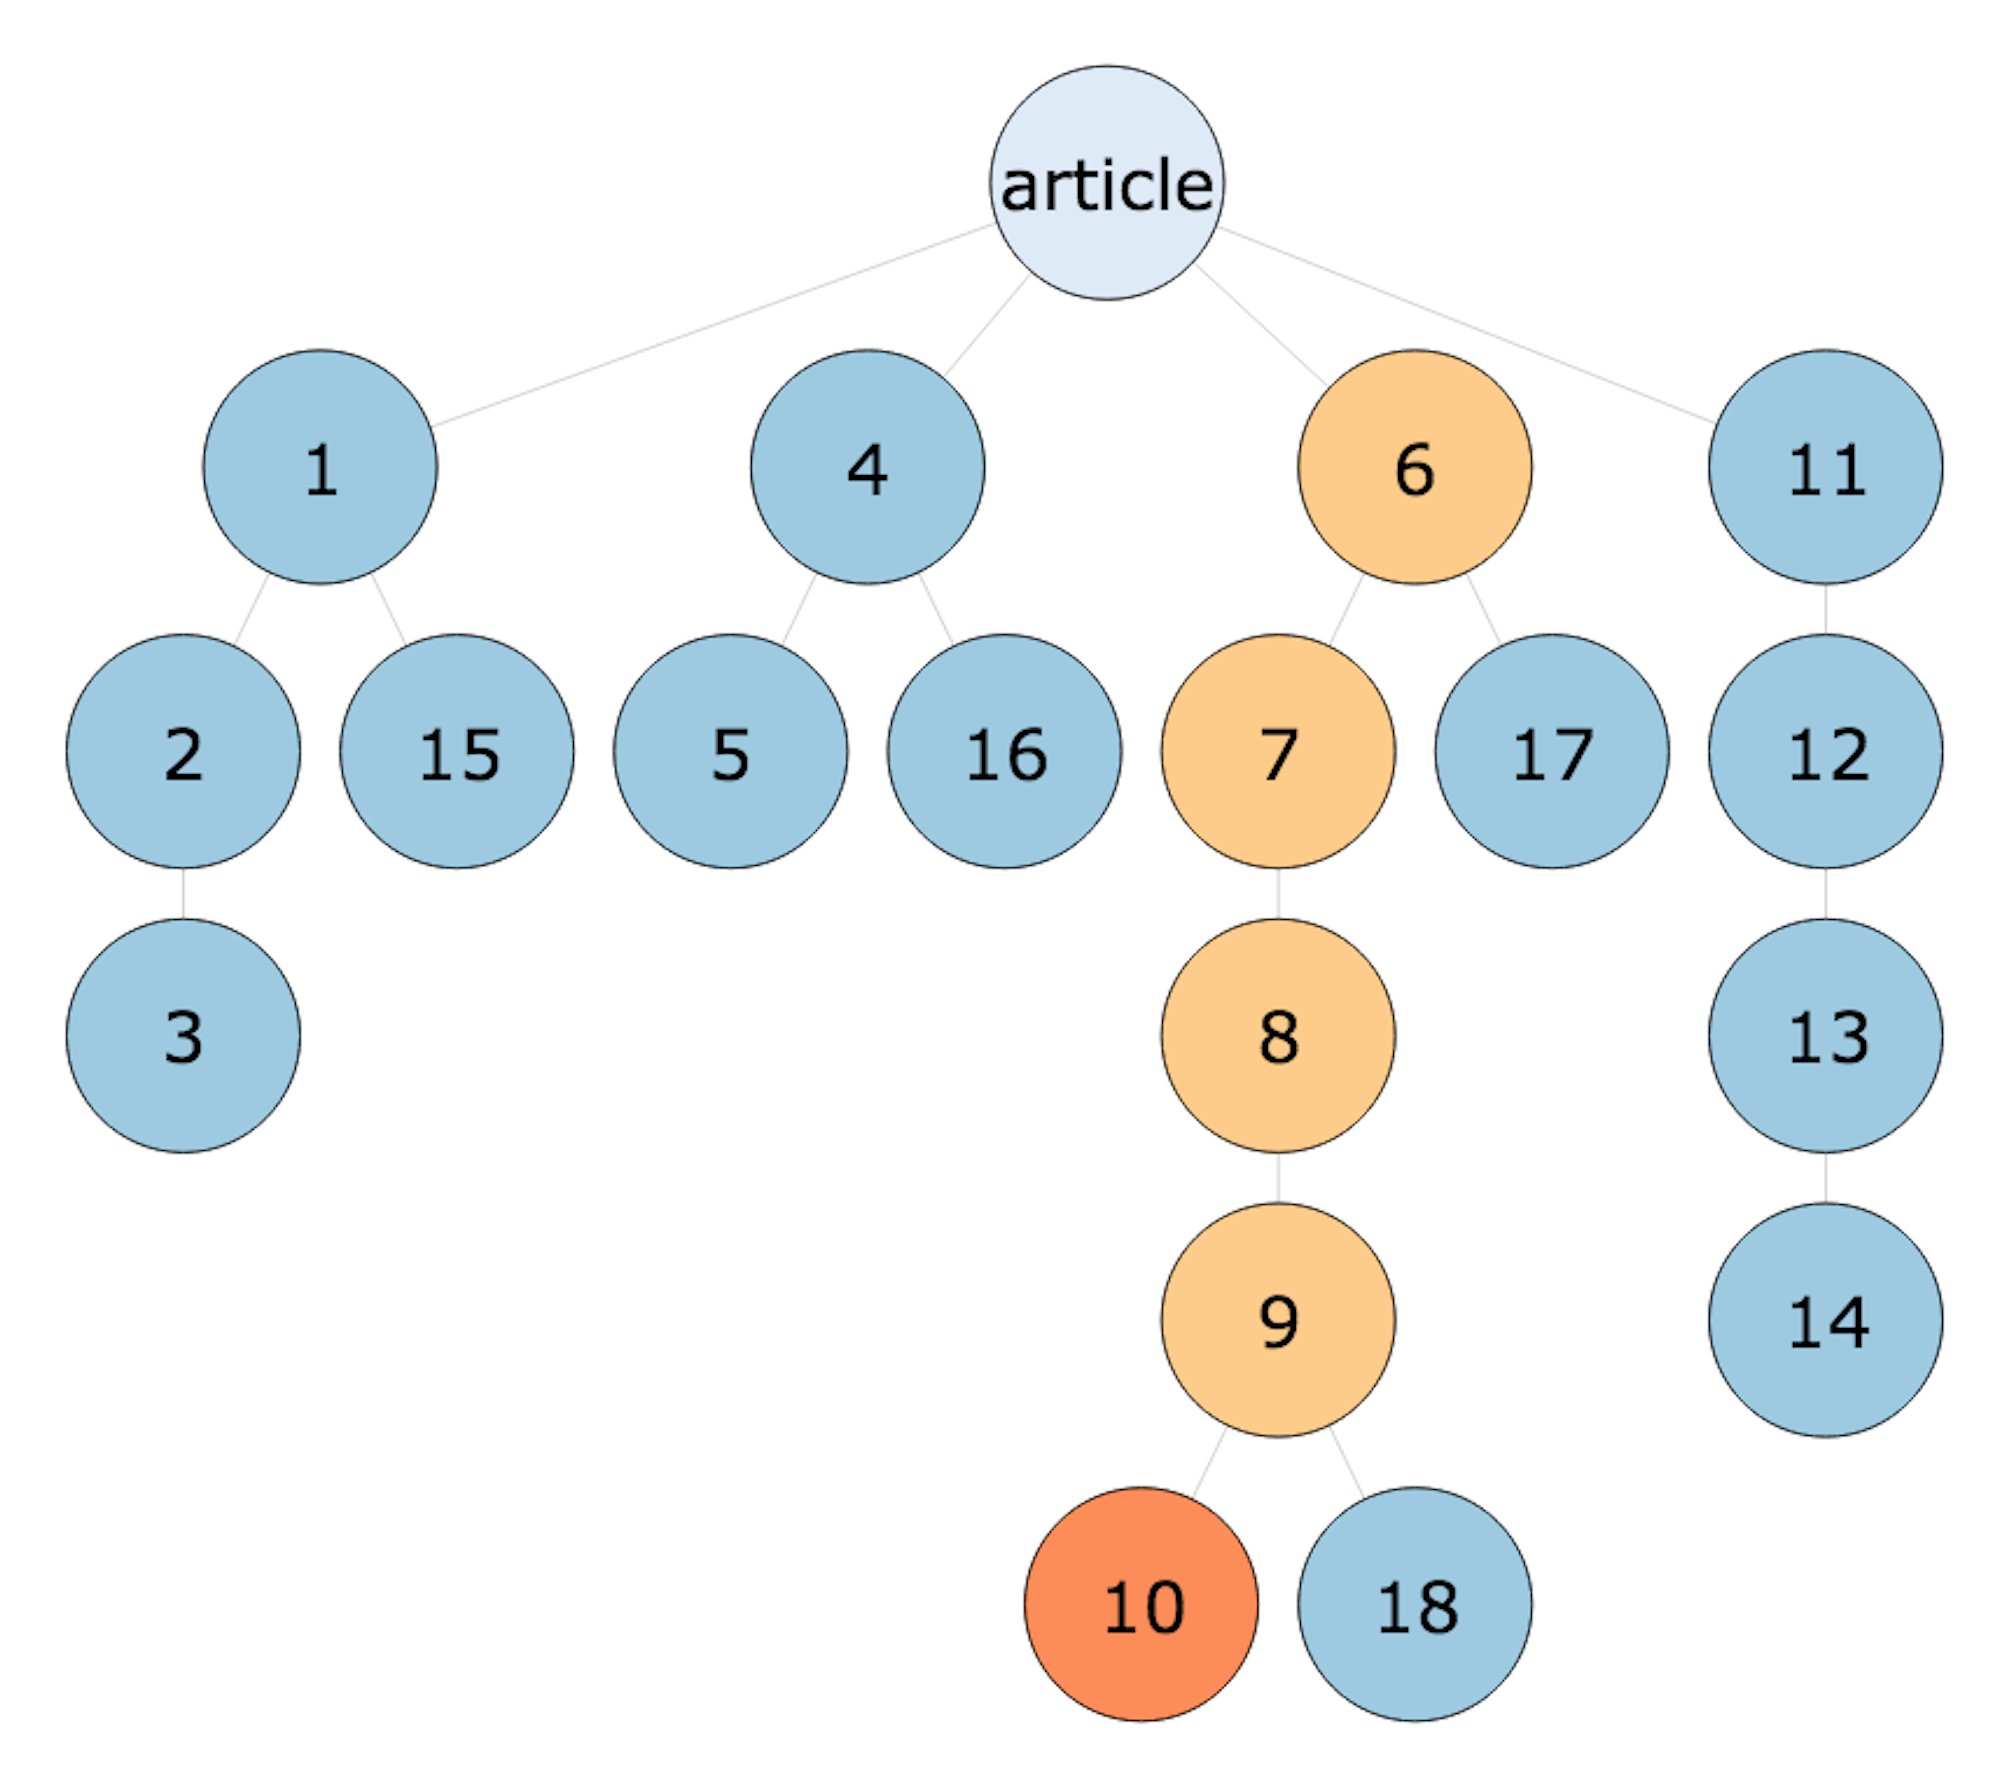
\includegraphics[width=0.5\textwidth]{images/approach/tree_10.png}
  \end{center}
  \caption{Prepending comments for tree-like comment structures is equivalent. The resulting sequence for Comment \textit{10} is: <t><c>\textbf{6}</c><c>\textbf{7}</c><c>\textbf{8}</c><c>\textbf{9}</c> <c>\textbf{10}</c></t>}
   \label{fig:appr_tree_pp}
\end{figure}

We implemented\footnote{\url{https://github.com/jfilter/masters-thesis}} the preprocessing in Python with Pandas\footnote{\url{https://pandas.pydata.org}} and Dask\footnote{\url{https://dask.org}}.
For the language model we used ULMFIT.
However, it can be applied to any other language-model-based text classification method because the preprocessing remains the same.
Recurrent neural network such as LSTMs are especially powerful since last internal state of the LSTM is used for classification. The comment to classify is always the last comment in a chain.

\section{ULMFIT for German}
\label{sec:ulmfit_for_de}

A general language model is required for using ULMFIT for text classification.
Since there does not exists a German pre-trained language model, we create one. Only with it, can we classify German comments of OMPC.

There has been effort to adapt ULMFIT to German but to no avail~\cite{ulmfit-germeval18}.
A first requirement is the existence of long, high-quality German texts.
It is important that the texts are long in order to learn long-term dependencies.
This allows the language model to get a deeper understanding of German.
We use a dump\footnote{\url{https://dumps.wikimedia.org}} of the entire German Wikipedia and extract the article's text with WikiExtractor\footnote{\url{https://github.com/attardi/wikiextractor}}.
To gather more data, we use news articles\footnote{In regard to ethical considerations, we note that we do not have the consent of the journalists who wrote the articles. However, journalists work in commission of a newspaper and no private information is attached to an article. And unlike for news comments, journalists know that their articles get processed automatically by, i.e., search engines.}.
We crawl news articles with News-Please\footnote{\url{https://github.com/fhamborg/news-please}} from several regional and national German newspaper.
Only documents with a length of at least 500 characters are kept.
The result is a collection of $3.278.657$ documents with altogether $1.197.060.244$ tokens. Compared to English, German is highly inflective.
And the language allows the construction of endless combination of compound nouns.
So a simple word-based approach would result in a large vocabulary.
It is encouraged to keep the vocabulary small, because in the last layer in a neural language model, a softmax activation function is computed over each entry in the vocabulary.
This is computationally intensive and a small vocabulary greatly speeds up the training process.
One way to do it, is to split words into sub-word units.
For instance, Byte-Pair Encoding (BPE) by Sennrich~et~al.~\cite{P16-1162} achieves this.
This is a compromise between word-based and character-based approaches.
The size of the vocabulary of sub-word units is fixed.
So the size of sub-units depend on the vocabulary size.
The smaller the vocabulary, the shorter the sub-word units.
Czapla~et~al.~\cite{czapla2018universal} successfully applied BPE to ULMFIT for Polish.
Since the splitting of word in sub-words is a model (or embedding) on its own, we can use a pre-trained model.
Heinzerling and Strube~\cite{heinzerling2018bpemb} provide pre-trained sub-word models\footnote{\url{https://nlp.h-its.org/bpemb}} for 275 languages.
The authors provide models for the vocabulary size from $1.000$ to $200.000$.
For Polish, Czapla et al. achieved the best results with vocabulary of $20.000$.
Since Polish and German are both Indo-Germanic languages, a parameter in the similar range should apply for German as well.
We choose a the German model with fixed vocabulary size of $25.000$.

\newpage

It follows an example of how it breaks up the German sentence
\begin{quote}
 ``\textit{Zeitungskommentare sind eine hervorragende M\"oglichkeit zum Meinungsaustausch}''
 \end{quote}
 into sub-word units:

\begin{quote}
	[`\_zeitungs',
 `komment',
 `are',
 `\_sind',
 `\_eine',
 `\_hervor',
 `ragende',
 `\_m\"oglichkeit',
 `\_zum',
 `\_meinungs',
 `austausch',
  '.']
\end{quote}

For instance, the German composite noun \textit{Meinungsaustausch} is split into two sub-word units. The white space is replaced with a special underscore token. We have to follow the preprocessing steps of the pre-trained model. This includes that all text is lowercased and all digits are replaced by a 0.

To train it, we take the default configuration of the English language:
an embedding size of 400 and 3 layered LSTM with 1150 hidden activations per layer.
But we fully disable dropout.
The amount of data is large enough such thats a strong regularization is not needed.
We trained for five epochs which took three days on a single GTX1800ti, with a batch size of $128$. The learning rate is chosen automatically by the learning rate finder ($0.00744..$). The training curves are in Figure~\ref{fig:germanlm} and the final model achieves a perplexity of $33.88..$. The language model is published for further usage\footnote{\url{https://johannesfilter.com/ulmfit-for-german}}.

 \begin{figure}
  \begin{center}
    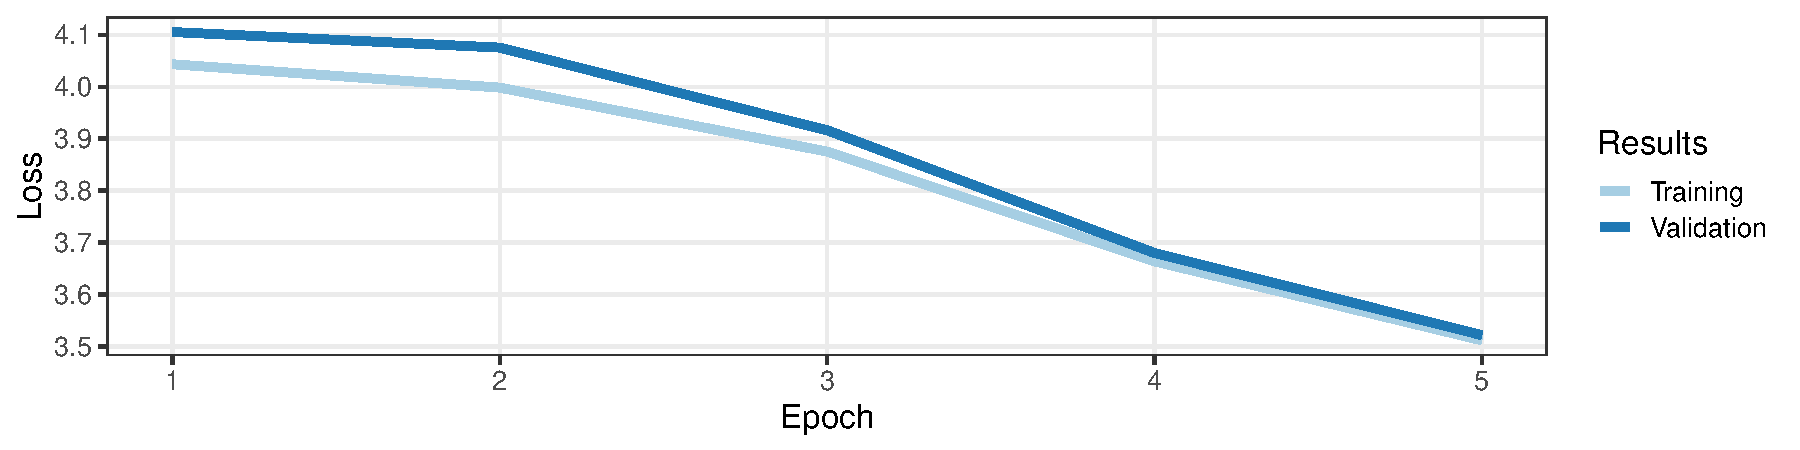
\includegraphics[width=\textwidth]{graphs/experiments/german_lm}
  \end{center}
	\caption{Training curves of the German language model.}
   \label{fig:germanlm}
\end{figure}


\chapter{Evaluation}
\label{sec:evaluation}

We evaluate our contributions on an English and a German datasets of comments datasets: YNACC and OMPC.
The datasets were introduced in Section~\ref{ch:datasets}.

\section{Experiments on Yahoo News Annotated Comments Corpus}

The Yahoo News Comment Corpus (YNACC) was intensively presented in Section~\ref{sec:datasets_ynacc}. We compare across three different approaches: baselines, conversation-agnostic models, and our conversation-aware models. 
\subsection{Setup}

For all experiments, we follow the dataset's preprocessing steps of the related work that reported values on YNACC~\cite{napoles2017finding}.
These were presented in Section~\ref{subsec:datasets_ynacc_description}.
Since there are already published results on this dataset, it sets our contribution into perspective.
We train a model for each category separately, as done by the related work.
The experiments and their results are managed via Sacred\footnote{\url{https://github.com/IDSIA/sacred}}.
The setup is different for each method so we describe them in detail in the following.

\subsubsection{Baselines}

We use three different methods as baseline: Naive Bayes, Ridge Regression and the FastText classifier.
All of them are linear classifiers.
The first two are traditional machine learning methods and the follow the bag-of-words idea.
The FastText classifier also considers N-gram of words.
It was introduced by Joulin et al.~\cite{E17-2068} and it outperforms even neural models while being up to $35.000$ times faster.
In addition to the data cleaning described in Section~\ref{subsec:ynacc_data_cleaning}, the tokens are lower-cased.
The default tokenizer of the respective implementation is used. For Naive Bayes and Ridge Regression, we use the Python package \textit{Scikit-Learn}\footnote{\url{https://scikit-learn.org}} in version 0.20.2. For Naive Bayes, we use \textit{MultinomialNB} with the default parameters. For Ridge Regression, we use the cross validation variant on the training data with, as well, the default parameters. For FastText, we use the Python wrapper of the official implementation\footnote{\url{https://github.com/facebookresearch/fastText/tree/master/python}}, version 0.2.0. Because the time to train is short, we use a random search for $1000$ times over the following uniformly distributed hyper-parameters: learning rate from 0 to 1, number of epochs from 5 to 50, N-grams for n from 1 to 5, minimum count for each token from 1 to 10.

\subsubsection{Conversation-agnostic Neural Models}
\label{ssssss:whaaatever}

We use two different language-model-based approaches as comparison models: ULMFIT and BERT. BERT is more advanced than ULMFIT, but it also requires more computation. Because of our financial constraints, we choose ULMFIT as the main reference model. For ULMFIT, we use the author's accompanied implementation in the FastAI library\footnote{\url{https://github.com/fastai/fastai}} in version 1.0.41. ULMFIT internally uses the SpaCy library\footnote{\url{https://spacy.io}} version 2.0 to tokenize the text. We as well clean our data as described in Section~\ref{subsec:ynacc_data_cleaning}. We choose a vocabulary size of $30k$ since it covers over $98.2\%$ of the tokens as shown in Figure~\ref{fig:word_based_anal}.
The use all special text preprocessing steps of the default FastAI implementation.
These are: tokens are lower cased, but for every uppercase word a special uppercase token is prepended. The same applies for all capitalized tokens. In addition, repeating tokens are replaced by a single token and the number of how often it was repeated gets prepended. For instance, ``yes !!!!!'' is transformed to ``yes xxrep 5 !''.

Before training the classifier, the pre-trained WikiText 103 language model needs to get fine-tuned. We choose the datasets of unlabeled comments together with the labeled training comments we noted as YC\textsubscript{LM} in Section~\ref{subsec:datasets_ynacc_description}. Characteristics of the datasets were presented in the section exhaustively. So we fine-tune the language model until overfitting. Even though the authors suggest to fine-tune cautiously, the number of unlabeled samples should be enough (about 200k).
We use random search over the following parameters: epochs 2 to 6, dropout factor from 0.8 to 1.1.
The learning rate scheduler is used to determine a learning rate.
There are 5 different kind of dropout in the model and the authors suggest to tune a specific dropout multiplier.
 And the layer factor, which sets different learning rate for each layer, is set to 2.6.
The authors obtained the magic numbers for the parameters with grid search and they recommend to follow them.
We only save the model with the best validation loss.
The validation set consists of the last $10\%$ of the discussion IDs.

For fine-tuning the classifier, we made the experience that results with the one cycle policy scheduling are unstable. The scheduler is suggested by the authors of the ULMFIT paper. The results varied a lot for different runs with the same parameters. This made it hard to compare the results and thus we abandon it. We use the standard Adam optimizer~\cite{kingma:adam} with the weight decay fix~\cite{loshchilov2017decoupled}.
We used a dropout multiplier of 0.6, 0.7 and 0.8 and a batch size of 64.
The learning rate is set to 0.001, since the learning rate finder did not yield useful results.
The maximum number of epochs is 200 but the learning is stopped, when the Cohen's Kappa score does not improve for 10 epochs (``early stopping''). Only the model with the best Cohen's Kappa score is saved. 

BERT by Devlin et al.~\cite{devlin2018bert} was already briefly mentioned in Section~\ref{sec:bgrd_tlwlm}. While we focus on ULMFIT in this work, the approach of BERT is similar. It requires more computation which is the reason we cannot use it for all our experiments. It is not feasible for us to fine-tune the language model on our domain of news comments. Thus, we use only a pre-trained BERT model. Out of familiarity with PyTorch, we use the port to PyTorch\footnote{\url{https://github.com/huggingface/pytorch-pretrained-BERT}}, which replicated the results of the original TensorFlow implementation. We chose the smaller English \textit{Bert Cased} model because we hypothesize that the casing in comments bears information. The approach operates on sub-word basis and did not require any preprocessing. First, we manually explored a range of useful hyper-parameters and then did a grid search over them. The parameters were: number of epochs from 3 to 10, the learning $5e^{-6}$, $5e^{-7}$, $5e^{-8}$.

\subsubsection{Prepend Previous}

For computational reason, we only evaluate Prepend Previous on the ULMFIT language model approach. The setup is the same as described for conversation-agnostic model in the previous section. Only the dropout multipliers are modified to 0.9, 1, 1.1, 1.2, 1.3. Comments are cut to 200, the total maximum token length is 1400 to optimize RAM usage. The learning rate is set to 0.001 and batch size to 64. Maximum number of epochs is 200 and early stopping is used.
The samples were truncated in the beginning. There are five different variations of Prepend Previous:

\begin{table}[H]
\caption{Variations of Prepend Previous}
\label{tab:eval_ynacc_setup}
\begin{tabular}{l l}
\toprule
Variation & Description \\
\midrule
TX\textsubscript{1} & text \\
TX\textsubscript{2} & text, the language model is not fine-tuned  \\
 HL\textsubscript{1} & text, headline is prepended to all top-level comments all the time \\
 HL\textsubscript{2} & text, headline is only prepended to top-level comments if they would be alone \\
 ART & text, headline, article (if available) \\
\bottomrule
\end{tabular}	
\end{table}

The difference between TX\textsubscript{1} and TX\textsubscript{2} is whether the fine-tuning of the language model has to be done on preprocessed comments (TX\textsubscript{1}) or on non-preprocessed comments (TX\textsubscript{2}). The language model for TX\textsubscript{2} was identical to the conversation-agnostic comparison models. For HL\textsubscript{1}, information about the article are always included. For HL\textsubscript{2}, the information was only included for top-level comments.
Since we do not have all articles, we cannot add all the articles for ART.

\subsection{Results}
\label{sec:exp_ynacc_results}

As metrics, we use F\textsubscript{1 micro}, which is equivalent to accuracy in this setup, F\textsubscript{1 macro} and, Cohen's Kappa (or short Kappa).
We explained Kappa in Section~\ref{sec:metrics} and gives a meaningful value even on unbalanced categories.
The full results including the test values are in Appendix~\ref{ch:ynacc_full}.
We only focus on validation results, since the related work does not report test results.
In addition, the test results differ greatly from the validation results across all models -- baselines as well as neural models.
For instance, Kappa increased in the category Audience by about 0.1 points for almost all models.
Also a simple ridge regression pushes the Kappa score from 0.52 to 0.66.
Even though the ridge regression baseline generally achieves poor results.
For all other categories, the performance deteriorates drastically on the test dataset.
For Off-topic, the differences are the most significant.
While on the validation sets, the Kappa score drops to below 0.2 for all models while performing on the validation set up to 0.48.
The further implications of these results will be discussed later.

In Table~\ref{tab:res1} are the results of the baseline compared to conversation-agnostic models.
The left side of the table consists of the comment's text only.
The right side of the text and a binary feature of whether a comment is a top-level comment or a reply.
This feature greatly improves the performance for the category Audience for all models.
However, for Agreement, Informative, Controversial and Off-topic the results decrease.
For the remaining categories are the differences negligible. In general, the FastText classifier outperformed the other baselines by far.
On the comment's text and reply, it achieved the best results on Audience by a margin of 0.04 F\textsubscript{1 micro} score.
BERT is overall the winner even though the language model was not fine-tuned on comments.
For Controversial, it outperforms other approaches by a margin of about 0.05 F\textsubscript{1 micro} score.
ULMFIT achieves slightly worse performance than BERT but still outperforms the baselines on the vast majority of categories.

\begin{table}
\small
\caption{Experiment results of baselines and conversation-agnostic comparison models on the YNACC validation dataset. The highst value for each row is highlighted. Since BERT~(BT) is out of competition, its values are underlined if it would have achieved the highest results. Naive Bayes~(NB), Ridge Regression~(RR), FastText Classifier~(FT), ULMFIT~(UF).}
\begin{tabular}{ l l l l l l l l l l l l}
\toprule
\multicolumn{2}{l}{} & \multicolumn{5}{c}{Text} & \multicolumn{5}{c}{Text + Reply} \\
\cmidrule(r){3-7}
\cmidrule(r){8-12}
Category & Metric &  NB & RR & FT & UF & BT & NB & RR & FT & UF & BT\\
\midrule
\addlinespace[2ex]
\multirow{3}{*}{Persuasive} & F\textsubscript{1 micro} & 0.814 & 0.855 & 0.871 & 0.845 & 0.864 & 0.835 & \textbf{0.876} & 0.874 & 0.830 & 0.862 \\
& F\textsubscript{1 macro} & 0.544 & 0.645 & 0.681 & 0.634 & \underline{0.721} & 0.578 & 0.655 & \textbf{0.694} & 0.684 & \underline{0.721} \\
& Kappa & 0.097 & 0.298 & 0.369 & 0.273 & 0.442 & 0.168 & 0.326 & \textbf{0.393} & 0.370 & \underline{0.443} \\ \addlinespace[2ex]
\multirow{3}{*}{Audience} & F\textsubscript{1 micro} & 0.686 & 0.698 & 0.741 & 0.746 & 0.795 & 0.783 & 0.809 & \textbf{0.876} & 0.834 & 0.831 \\
& F\textsubscript{1 macro} & 0.586 & 0.594 & 0.677 & 0.708 & 0.765 & 0.728 & 0.753 & \textbf{0.829} & 0.790 & 0.803 \\
& Kappa & 0.207 & 0.228 & 0.369 & 0.417 & 0.532 & 0.470 & 0.524 & \textbf{0.662} & 0.591 & 0.608 \\ \addlinespace[2ex]
\multirow{3}{*}{Agreement} & F\textsubscript{1 micro} & 0.885 & 0.879 & 0.902 & 0.907 & 0.903 & 0.885 & 0.885 & 0.905 & \textbf{0.912} & 0.903 \\
& F\textsubscript{1 macro} & 0.497 & 0.494 & 0.673 & \textbf{0.719} & 0.709 & 0.497 & 0.555 & 0.672 & 0.696 & \underline{0.727} \\
& Kappa & 0.046 & 0.035 & 0.357 & \textbf{0.444} & 0.423 & 0.046 & 0.140 & 0.357 & 0.404 & \underline{0.457} \\ \addlinespace[2ex]
\multirow{3}{*}{Informat.} & F\textsubscript{1 micro} & 0.818 & 0.818 & 0.816 & \textbf{0.866} & 0.862 & 0.826 & 0.821 & 0.821 & 0.847 & 0.845 \\
& F\textsubscript{1 macro} & 0.558 & 0.528 & 0.614 & \textbf{0.683} & \underline{0.748} & 0.553 & 0.494 & 0.623 & 0.679 & 0.717 \\
& Kappa & 0.136 & 0.087 & 0.233 & \textbf{0.378} & \underline{0.496} & 0.135 & 0.037 & 0.251 & 0.362 & 0.434 \\ \addlinespace[2ex]
\multirow{3}{*}{Mean} & F\textsubscript{1 micro} & 0.813 & 0.813 & 0.826 & \textbf{0.842} & \underline{0.849} & 0.811 & 0.813 & 0.823 & 0.840 & 0.835 \\
& F\textsubscript{1 macro} & 0.640 & 0.630 & 0.666 & 0.726 & 0.740 & 0.641 & 0.619 & 0.674 & \textbf{0.752} & 0.723 \\
& Kappa & 0.296 & 0.280 & 0.348 & 0.457 & 0.484 & 0.297 & 0.263 & 0.359 & \textbf{0.504} & 0.448 \\ \addlinespace[2ex]
\multirow{3}{*}{Controv.} & F\textsubscript{1 micro} & 0.663 & 0.641 & 0.687 & \textbf{0.706} & 0.735 & 0.691 & 0.703 & 0.704 & \textbf{0.706} & \underline{0.758} \\
& F\textsubscript{1 macro} & 0.639 & 0.574 & 0.644 & \textbf{0.675} & 0.700 & 0.661 & 0.590 & 0.663 & 0.672 & \underline{0.722} \\
& Kappa & 0.286 & 0.149 & 0.289 & \textbf{0.353} & 0.400 & 0.325 & 0.212 & 0.326 & 0.346 & \underline{0.445} \\ \addlinespace[2ex]
\multirow{3}{*}{Disagree.} & F\textsubscript{1 micro} & 0.634 & 0.646 & 0.703 & 0.756 & 0.739 & 0.660 & 0.701 & 0.737 & \textbf{0.778} & 0.777 \\
& F\textsubscript{1 macro} & 0.626 & 0.639 & 0.682 & 0.745 & 0.729 & 0.654 & 0.687 & 0.724 & \textbf{0.772} & 0.770 \\
& Kappa & 0.254 & 0.280 & 0.368 & 0.491 & 0.459 & 0.312 & 0.375 & 0.448 & \textbf{0.546} & 0.540 \\ \addlinespace[2ex]
\multirow{3}{*}{Off-topic} & F\textsubscript{1 micro} & 0.682 & 0.663 & 0.687 & \textbf{0.749} & 0.737 & 0.704 & 0.668 & 0.680 & 0.706 & 0.740 \\
& F\textsubscript{1 macro} & 0.543 & 0.539 & 0.608 & \textbf{0.670} & 0.663 & 0.601 & 0.625 & 0.609 & 0.644 & \underline{0.676} \\
& Kappa & 0.127 & 0.105 & 0.222 & \textbf{0.353} & 0.334 & 0.222 & 0.252 & 0.222 & 0.290 & \underline{0.357} \\ \addlinespace[2ex]
\multirow{3}{*}{Sentiment} & F\textsubscript{1 micro} & 0.548 & 0.533 & 0.564 & 0.622 & 0.633 & 0.554 & 0.536 & 0.577 & \textbf{0.628} & \underline{0.638} \\
& F\textsubscript{1 macro} & 0.248 & 0.290 & 0.381 & 0.417 & \underline{0.471} & 0.256 & 0.303 & 0.358 & \textbf{0.448} & 0.450 \\
& Kappa & 0.099 & 0.102 & 0.228 & 0.315 & \underline{0.377} & 0.107 & 0.133 & 0.232 & \textbf{0.322} & 0.374 \\ \addlinespace[2ex]
\midrule
\addlinespace[2ex]
\multirow{3}{*}{Average}  & F\textsubscript{1 micro} & 0.727 & 0.727 & 0.755 & 0.782 & 0.790 & 0.749 & 0.756 & 0.777 & \textbf{0.786} & \underline{0.798} \\ & F\textsubscript{1 macro} & 0.542 & 0.548 & 0.625 & 0.664 & 0.694 & 0.574 & 0.586 & 0.649 & \textbf{0.681} & \underline{0.701} \\ & Kappa & 0.172 & 0.173 & 0.309 & 0.386 & 0.438 & 0.231 & 0.251 & 0.361 & \textbf{0.415} & \underline{0.456} \\ \addlinespace[2ex]
\bottomrule
\end{tabular}
\label{tab:res1}
\end{table}

\begin{table}
%\small
\caption{Experiment results on the YNACC validation dataset comparing conversation-agnostic models with conversation-aware models. The former group of models stems from Table~\ref{tab:res1}. The latter were explained in Table~\ref{tab:eval_ynacc_setup}. The highest value in each row is highlighted.}
\begin{tabular}{ l l l l l l l l l l}
\toprule
\multicolumn{2}{l}{} & \multicolumn{3}{c}{Conversation-agnostic} & \multicolumn{5}{c}{Conversation-aware} \\
\cmidrule(r){3-5}
\cmidrule(r){6-10}
Category & Metric & UF\textsubscript{text} & FT\textsubscript{reply} & UF\textsubscript{reply} & TX\textsubscript{1} & TX\textsubscript{2} & HL\textsubscript{1} & HL\textsubscript{2} & ART\\
\midrule
\addlinespace[2ex]
\multirow{3}{*}{Persuasive} & F\textsubscript{1 micro} & 0.845 & \textbf{0.874} & 0.830 & 0.847 & 0.845 & 0.847 & 0.871 & 0.811 \\
& F\textsubscript{1 macro} & 0.634 & 0.694 & 0.684 & 0.703 & 0.674 & 0.688 & \textbf{0.720} & 0.651 \\
& Kappa & 0.273 & 0.393 & 0.370 & 0.407 & 0.348 & 0.378 & \textbf{0.442} & 0.303 \\ \addlinespace[2ex]
\multirow{3}{*}{Audience} & F\textsubscript{1 micro} & 0.746 & \textbf{0.876} & 0.834 & 0.836 & 0.827 & 0.839 & 0.826 & 0.833 \\
& F\textsubscript{1 macro} & 0.708 & \textbf{0.829} & 0.790 & 0.796 & 0.777 & 0.794 & 0.797 & 0.785 \\
& Kappa & 0.417 & \textbf{0.662} & 0.591 & 0.600 & 0.569 & 0.600 & 0.596 & 0.583 \\ \addlinespace[2ex]
\multirow{3}{*}{Agreement} & F\textsubscript{1 micro} & 0.907 & 0.905 & 0.912 & \textbf{0.921} & 0.912 & \textbf{0.921} & 0.915 & 0.909 \\
& F\textsubscript{1 macro} & 0.719 & 0.672 & 0.696 & 0.761 & 0.746 & 0.761 & \textbf{0.763} & 0.731 \\
& Kappa & 0.444 & 0.357 & 0.404 & 0.526 & 0.494 & 0.526 & \textbf{0.529} & 0.466 \\ \addlinespace[2ex]
\multirow{3}{*}{Informative} & F\textsubscript{1 micro} & \textbf{0.866} & 0.821 & 0.847 & 0.847 & 0.843 & 0.859 & 0.845 & 0.826 \\
& F\textsubscript{1 macro} & 0.683 & 0.623 & 0.679 & \textbf{0.695} & 0.672 & 0.693 & 0.690 & 0.666 \\
& Kappa & 0.378 & 0.251 & 0.362 & 0.391 & 0.348 & \textbf{0.392} & 0.381 & 0.334 \\ \addlinespace[2ex]
\multirow{3}{*}{Mean} & F\textsubscript{1 micro} & 0.842 & 0.823 & 0.840 & 0.814 & 0.840 & \textbf{0.845} & 0.838 & 0.826 \\
& F\textsubscript{1 macro} & 0.726 & 0.674 & \textbf{0.752} & 0.726 & 0.724 & 0.749 & 0.738 & 0.727 \\
& Kappa & 0.457 & 0.359 & \textbf{0.504} & 0.453 & 0.453 & 0.500 & 0.477 & 0.455 \\ \addlinespace[2ex]
\multirow{3}{*}{Controversial} & F\textsubscript{1 micro} & 0.706 & 0.704 & 0.706 & 0.728 & 0.725 & 0.727 & 0.728 & \textbf{0.739} \\
& F\textsubscript{1 macro} & 0.675 & 0.663 & 0.672 & 0.679 & 0.672 & 0.684 & 0.686 & \textbf{0.689} \\
& Kappa & 0.353 & 0.326 & 0.346 & 0.360 & 0.346 & 0.369 & 0.372 & \textbf{0.380} \\ \addlinespace[2ex]
\multirow{3}{*}{Disagreement} & F\textsubscript{1 micro} & 0.756 & 0.737 & 0.778 & \textbf{0.794} & 0.782 & 0.792 & 0.785 & 0.763 \\
& F\textsubscript{1 macro} & 0.745 & 0.724 & 0.772 & \textbf{0.786} & 0.773 & 0.783 & 0.777 & 0.756 \\
& Kappa & 0.491 & 0.448 & 0.546 & \textbf{0.572} & 0.547 & 0.567 & 0.554 & 0.513 \\ \addlinespace[2ex]
\multirow{3}{*}{Off-topic} & F\textsubscript{1 micro} & 0.749 & 0.680 & 0.706 & 0.754 & 0.763 & 0.758 & \textbf{0.770} & 0.753 \\
& F\textsubscript{1 macro} & 0.670 & 0.609 & 0.644 & 0.722 & 0.712 & 0.702 & \textbf{0.740} & 0.711 \\
& Kappa & 0.353 & 0.222 & 0.290 & 0.444 & 0.426 & 0.407 & \textbf{0.481} & 0.423 \\ \addlinespace[2ex]
\multirow{3}{*}{Sentiment} & F\textsubscript{1 micro} & 0.622 & 0.577 & 0.628 & \textbf{0.647} & 0.615 & 0.603 & 0.610 & 0.608 \\
& F\textsubscript{1 macro} & 0.417 & 0.358 & \textbf{0.448} & 0.408 & 0.420 & 0.409 & 0.411 & 0.421 \\
& Kappa & 0.315 & 0.232 & 0.322 & \textbf{0.361} & 0.321 & 0.318 & 0.328 & 0.324 \\ \addlinespace[2ex]
\midrule
\addlinespace[2ex]
\multirow{3}{*}{Average}  & F\textsubscript{1 micro} & 0.782 & 0.777 & 0.786 & \textbf{0.798} & 0.794 & \textbf{0.798} & \textbf{0.798} & 0.785 \\ & F\textsubscript{1 macro} & 0.664 & 0.649 & 0.681 & 0.697 & 0.685 & 0.695 & \textbf{0.702} & 0.681 \\ & Kappa & 0.386 & 0.361 & 0.415 & 0.457 & 0.428 & 0.450 & \textbf{0.462} & 0.420 \\ \addlinespace[2ex]
\bottomrule
\end{tabular}
\label{tab:res2}
\end{table}


In Table~\ref{tab:res2} are the results of conversation-aware model in comparison to three best-scoring conversation-agnostic models from Table~\ref{tab:res1}.
On average, context-aware models achieve superior results.
The F\textsubscript{1 micro}, F\textsubscript{1 micro} and Kappa scores increased by 1.53\%, 3.08\% and 11.33\%, respectivly.
Off-topic is the greatest beneficiary with an increase by 36.26\% in Kappa score.
The change in percent is visualized in Figure~\ref{fig:res_changes}.
However, there are differences among the categories.
For Audience and Mean, the performance decreased.
For others such as Agreement, Disagreement, Controversial and Off-topic all metrics improved.
We tested several variations of Prepend Previous.
The first question was whether it is important to fine-tune the language model with preprocessed tokens.
TX\textsubscript{1} outperforms TX\textsubscript{2} in almost all metrics for all categories.
Then, it seems that adding more information does not always seem to help.
Especially, adding information about the article does in some cases decrease the results.
The results of HL\textsubscript{1} and HL\textsubscript{2} differ only slightly.
Only for Persuasive and Off-Topic HL\textsubscript{2} outperforms clearly.
Adding even more information, such as the whole article text, seem to decrease the performance almost all categories.
Only Controversial achieved the best results for ART.
In order to understand the differences for the conversation-aware models, we investigate the effect of it at the example of the category Off-topic.
The conversation-aware model outperform conversation-agnostic models especially when the comments is short. For longer comments, the performance decreased. This is visualized in Figure~\ref{fig:exp_acc_len}. The overall performance increased since the majority of the comments is short (Figure~\ref{fig:len_com}).

\begin{figure}
  \begin{center}
    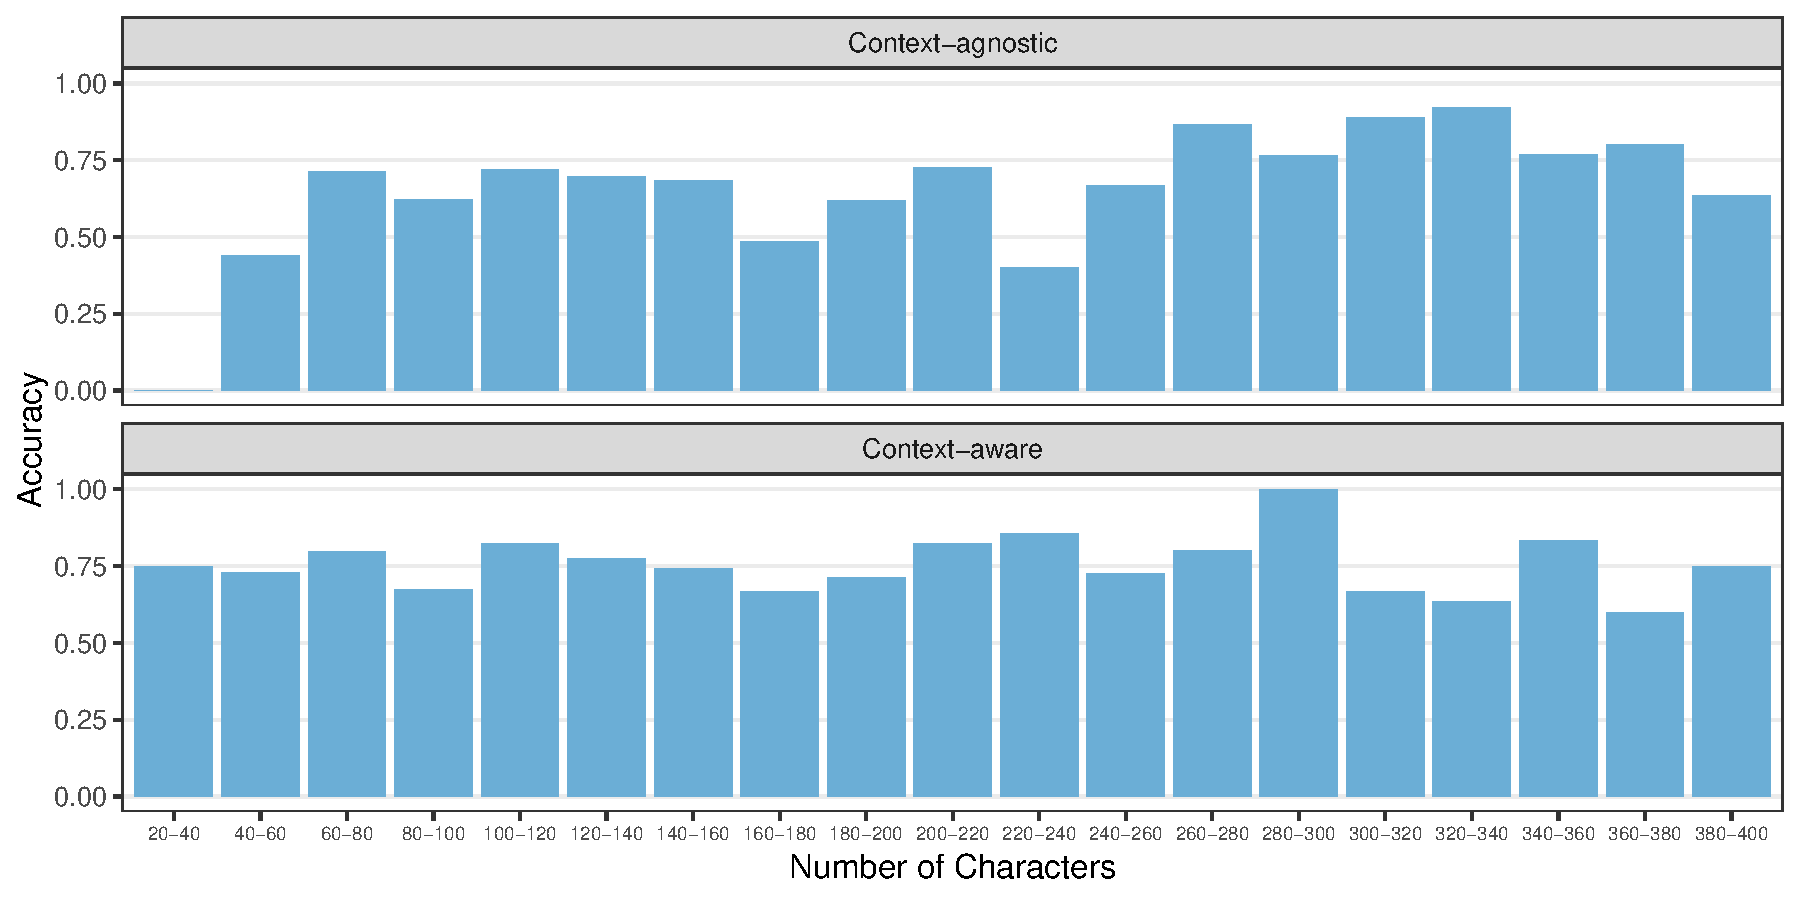
\includegraphics[width=1\textwidth]{graphs/experiments/length_acc.pdf}
  \end{center}
  \caption{A comparison of the performance between a conversation-agnostic model (only reply) with a conversation-aware model (PP, headline only root) in regard to length of comments.}
   \label{fig:exp_acc_len}
\end{figure}


\begin{figure}
  \begin{center}
    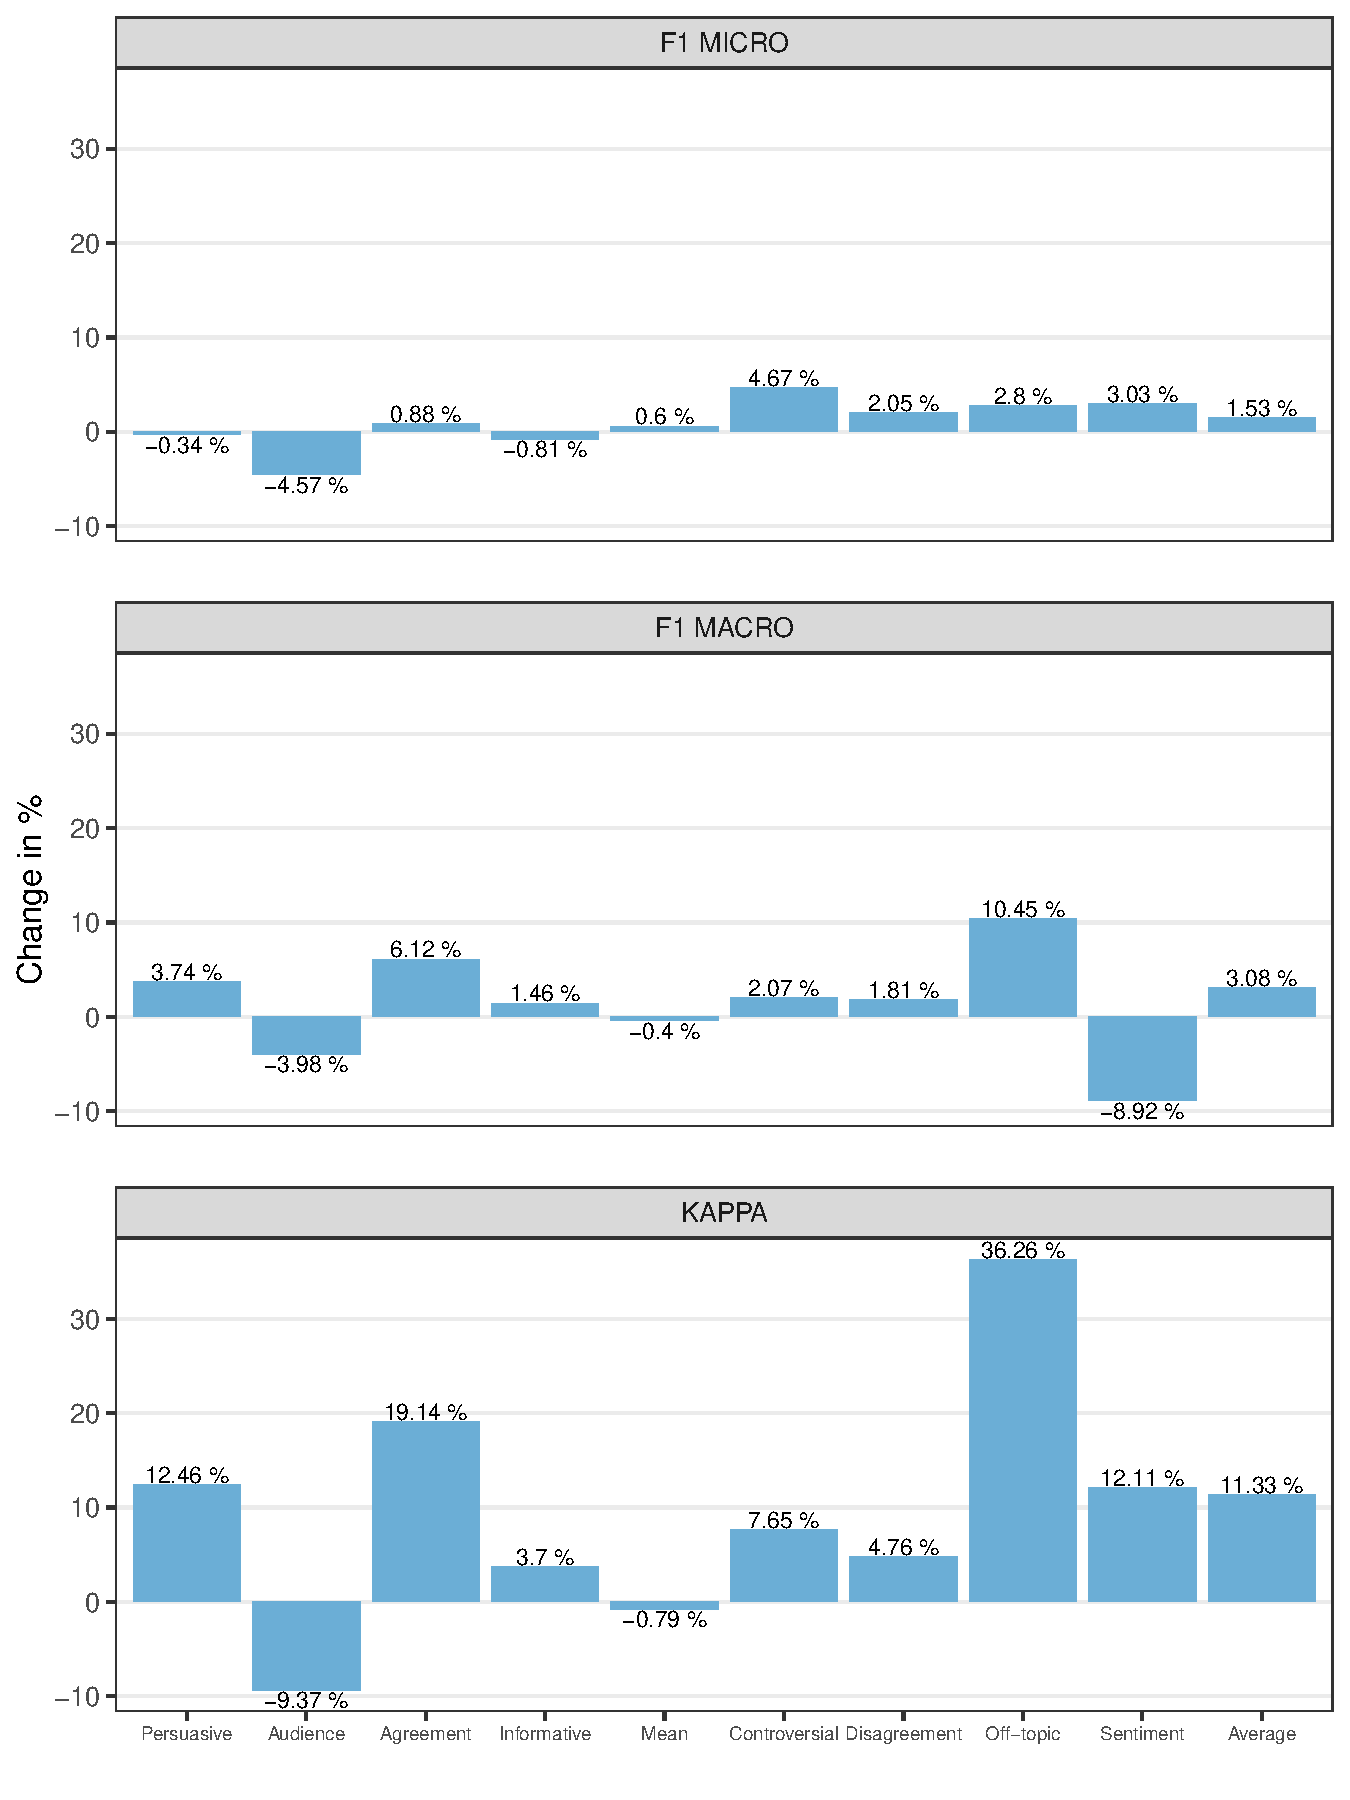
\includegraphics[width=1\textwidth]{graphs/experiments/changes.pdf}
  \end{center}
  \caption{The change in percent of the best conversation-agnostic model vs the best conversation-aware model based on Kappa.}
   \label{fig:res_changes}
\end{figure}

Finally, we speculate whether we have outperformed previously reported values.
Unfortunately, we cannot be sure how exactly the metrics were created.
The values were presented and also discussed in Section~\ref{subsec:ynacc_reported}.
The Kappa values that are presented come from this section.
We focus on Kappa to compare the performance of a model with a single metric.
There are multiple categories where the reported results are either impressive or poor:
Persuasive (0.79 or -0.173), Mean (0.693 or -0.238), Agreement (0.728 or -0.184), Off-topic (0.474 or -0.237).
For Audience, the values are so clear (0.816 or 0.575).
It is hard to make a definite statement about them.
However, for other categories we outperformed them clearly.
We can say for sure that we have outperformed YNACC for Controversial (0.158 or -0.024) and Disagreement (0.365 or 0.009).
The authors reveal in their publication that Informative (0.703 or -0.25) is below their ridge regression baseline.
So the value of 0.703 is impossible.
This means we have outperformed them clearly.
Also Sentiment with a reported F\textsubscript{1} of 0.43 is below our results of over 0.6 for the majority of approaches.
Since this is a four-class setup, the values ought to be averaged in some way.
We do not know how but we outperformed them in any way.


\subsection{Discussion}


The issue concerning the reported values makes it hard to compare our results.
However, we could demonstrate that we outperformed previous results in at  least three categories.
We were mainly reporting on the results on the validation set.
This has two reasons.
We want to set our work into perspective -- even this was only possible for three categories.
Moreover, the test values the dropped across all models considerably.
Generally, it is advised to report values on the test set, because it is likely that one has overfit parameters on the validation set.
So the validation results must be considered carefully.
However, our question was primarily whether it is essential to consider the conversational context is important.
And this can be answered by working on the validation as well as test results.
And the test sets contains further uncertainty, since they were annotated from a different group of people than the training and validation set.
Also the unnecessary noise of randomly assigning samples to classes, where  no majority wins is a problem.
So the drop in the models can be explained by the noise in the data as characteristics of the data.
In news comments, the words greatly differ from article to article.
More annotated data is needed to create better datasets to create more accurate results.

Our results allow to believe that the conversational context helped for certain categories.
It is not needed for all categories.
But for categories, that relate in some way to previous comments, the performance with context increased.
This allowed the model to get a deeper understanding of news comments.
To decide whether a comments agrees or disagrees, it helps to understand what was written before.
Also to decide whether a comment is off-topic, the previous comment help to make clear what the actual topic is.
That adding information about the article decreases the performance, may a problem of this approach.
Information about an article may duplicated immensely in the trainings sets.
So here Prepend Previous has some serious short-comings.
Further research is needed to overcome this.
Using separate sub-networks for the article and the comment may help.


\section{Experiments on One Million Posts Corpus}

In this section, we conduct two experiment on the dataset of German news which was described in Section~\ref{sec:ompc_ds}.

\subsection{Setup}

The conversation-agnostic model follows the same setup as already described in Section~\ref{ssssss:whaaatever} for experiments on YNACC.
A general German language model is required and it was presented in Section~\ref{sec:ulmfit_for_de}.
The language model is fine-tuned on the unlabeled comments until overfitting.
The OMPC datasets as well contains cross validation folds.
We re-use these to compare our results.
The model is trained for 100 epochs but stopped if the Kappa score did not improve for over 40 epochs.
The test value of the last epoch is used to determine a fold's performance.
The following parameters were used: a dropout multiplier of 0.8, a learning rate of 0.001, and a batch size of 128.

For the conversation-aware model, the comments were preprocessed with Prepend Previous.
Since the comments were originally created in a tree-like discussion structure, the Prepend Previous differs from YNACC.
It can happen that an intermediate-comment can have more than one child.
Thus this comment appears multiple times in the samples.
To avoid duplicates of those comments, all comment chains are truncated to 400 tokens.
This should ensure that the number of duplications is low.
Since classes are unbalanced, the loss was weighted according to the distribution of classes in the appropriate fold.

\subsection{Results}
\label{sec:ompc_results}

The results are presented in Table~\ref{tab:res3}.
We follow the metrics of related literature and show the Precision, Recall and F\textsubscript{1} in regard to the minority class.
The conversation-aware model achieved lower results than a conversation-agnostic model in all categories.
However, the context-agnostic model outperformed previously reported results besides for the categories Feedback and Off-topic.
There does not exists a previously reported result for Neutral.
H{\"a}ring et al.~\cite{haring2018addressed} only reported results for Feedback.
The best value of all of the experiments by Schabus et al.~\cite{schabus_academic-industrial_nodate} are chosen as reference.
The F\textsubscript{1} increased for Positive and Inappropriate by 79.3\% and 25.1\%, respectively.

\begin{table}
\caption{The cross-validation results on OMPC. The best models by Schabus et al.~\cite{schabus_academic-industrial_nodate}, based on their F\textsubscript{1} score, are chosen as reference. H{\"a}ring~et al.\cite{haring2018addressed} only report results for Feedback. Only the F\textsubscript{1} score is highlighted}
\begin{tabular}{ l l l l l l}
\toprule
Category & Metric & Schabus~\cite{schabus_academic-industrial_nodate} & H{\"a}ring~\cite{haring2018addressed} & Context-agnostic & Context-aware\\
\midrule
\addlinespace[2ex]
\multirow{3}{*}{Negative} & Precision & 0.6112 & & 0.6044 & 0.5802 \\
& Recall & 0.6014 & & 0.6168 & 0.5311 \\
& F\textsubscript{1} & 0.6063 & & \textbf{0.6089} & 0.5290 \\ \addlinespace[2ex]
\multirow{3}{*}{Neutral} & Precision & & & 0.6124 & 0.5478 \\
& Recall & & & 0.6155 & 0.5305 \\
& F\textsubscript{1} & &  & \textbf{0.6073} & 0.5089 \\ \addlinespace[2ex]
\multirow{3}{*}{Positive} & Precision & 0.1020 & & 0.4850 & 0.3299 \\
& Recall & 0.3488 & & 0.2422 & 0.1797 \\
& F\textsubscript{1} & 0.1579 & & \textbf{0.2831} & 0.1418 \\ \addlinespace[2ex]
\multirow{3}{*}{Off-topic} & Precision & 0.2472 & & 0.4637 & 0.4344 \\
& Recall & 0.6086 & & 0.2771 & 0.2169 \\
& F\textsubscript{1} & \textbf{0.3516} & & 0.3431 & 0.2603 \\ \addlinespace[2ex]
\multirow{3}{*}{Inappr} & Precision & 0.1340 & & 0.4585 & 0.4531 \\
& Recall & 0.5776 & & 0.2010 & 0.1358 \\
& F\textsubscript{1} & 0.2175 & & \textbf{0.2720} & 0.1939 \\ \addlinespace[2ex]
\multirow{3}{*}{Discrim} & Precision & 0.1207 & & 0.3288 & 0.4881 \\
& Recall & 0.5922 & & 0.1512 & 0.1080 \\
& F\textsubscript{1} & 0.2005 & & \textbf{0.2037} & 0.1596 \\ \addlinespace[2ex]
\multirow{3}{*}{Feedback} & Precision & 0.5311 & 0.85 & 0.8178 & 0.8424 \\
& Recall & 0.7356 & 0.83 & 0.6383 & 0.5362 \\
& F\textsubscript{1} & 0.6168 & \textbf{0.84} & 0.7099 & 0.6443 \\ \addlinespace[2ex]
\multirow{3}{*}{Personal} & Precision & 0.6247 & & 0.8787 & 0.7329 \\
& Recall & 0.8123 & & 0.6271 & 0.6516 \\
& F\textsubscript{1} & 0.7063 & & \textbf{0.7188} & 0.6670 \\ \addlinespace[2ex]
\multirow{3}{*}{Argument} & Precision & 0.5457 & & 0.7612 & 0.6854 \\
& Recall & 0.7652 & & 0.5644 & 0.5592 \\
& F\textsubscript{1} & 0.6371 & & \textbf{0.6430} & 0.6026 \\ \addlinespace[2ex]
\bottomrule
\end{tabular}
\label{tab:res3}
\end{table}

\subsection{Discussion}

Further research is needed to evaluate whether the conversational context improves the performance for the OMPC datasets.
The current results for context-aware models are far below conversation-agnostic models.
This may have various reasons.
The amount of annotated is low and especially the number of test samples with for the most categories of about 300 is low.
This leads to fluctuating performances across the folds.
Different variations of early stopping should be explored.
Setting the same parameters for all folds may not have been the best decision.
For some folds, the model needs to get more carefully trained with more regularization.
In other folds, the model did not converge at all.
To tune hyper-parameters, the training folds should be split into an addition validation fold.
Then, the parameters need to get tuned on the validation set before measuring the final performance on the test set.
Nevertheless, the conversation-agnostic model outperformed the featured-based models by Schabus in almost all cases.
Even though there is, i.e., no information about the casing in the text.
The casing in news comments bears information.
So for the future, a German language model with casing should be trained.




\chapter{Conclusions and Future Work}
\label{chp:conclusions}

In this master's thesis, we investigated the importance of the conversational structure for automatically classifying news comments.
We used the state-of-the-art methods for text classification which involve transfer learning with language models.
Language models create powerful text representation as a by-product of being trained to predict the next word based on previous words.
We introduced the preprocessing technique \textit{Prepend Previous} to exploit the sequential structure of news comments.
Prepending previous comments to each comment allows the language model to grasp the whole conversation around a news article.
We demonstrate how Prepend Previous can be applied to ULMFIT, but it could be applied to any language-model-based classification technique.

We successfully conducted experiments on the English news comments dataset YNACC.
With conversation-aware models, the performances for several categories increased over conversation-agnostic models.
For instance, to detect whether a comment agrees or disagrees with another comment benefits from our technique.
But also the results for other categories increased by the conversation-awareness: Off-topic, Controversial, Persuasive, or Sentiment.
We conclude that conversation-aware models increase the classification performance for categories that require a deeper understanding of a comment's surrounding.
With the right preprocessing steps, we showed that language models are able to accomplish this.
We as well investigated whether adding information about the article improves the models even further.
This is mostly not the case.
More research is needed to build models that relate comments to their article.
Our method has the disadvantage of duplicating information about the article in multiple training samples.
This may lead to overfitting on, i.e., the headline of a news article.
It can be overcome by introducing separate models for encoding information about the article and comments.
In addition, we applied the approach to German news comments dataset OMPC.
But more experiments are required to draw conclusions in regard to the conversation-awareness.
However, we successfully applied ULMFIT to them and improve on previously reported results in six out of nine categories.
We publish a German language model for further usage.

There are also some drawbacks of Prepend Previous.
By prepending comments, the size of each sample grew immensely, in our experiments by a factor of 10.
A language model by itself takes considerable resources to train and  this modification increases them even further.
So for future work, a mechanism to reduce training time should be explored.
One could think of incorporating ``skip connections'' that let the model skip over previous comments if they are not important.
It is rarely the case, that all previous comments are essential.
This would also help to reduce the ecological footprint.
One other direction is improving language models by adding metadata.
Text rarely appears in isolation so metadata such as timestamps should be incorporated.
Additional performance improvements can be gained by using recent Transformer-based language models, i.e., the Transformer-Xl~\cite{DBLP:journals/corr/abs-1901-02860}.
They outperform LSTM-based language models and should capture the long-term dependencies of news comments conversations better.


The lack of high-quality datasets of news comments was a major problem of this work.
Datasets, especially annotated ones, are an integral part of machine learning.
Without carefully created datasets, the model cannot learn the characteristics of the samples.
For news comments datasets, the number of annotated comments is low (<10k) and the datasets have issues as noted in Section~\ref{ch:datasets}.
For future work, a large corpus of annotated comments would help the research field immensely.
The already annotated data could simplify the process of creating new training samples.
First, one has to train a model on the available annotated data.
Second, the model predicts the classes of unlabeled comments.
Third, annotators need to verify the comments manually.
The process is significantly shorter then planning and conducting annotations ``from scratch''.
The German dataset OMPC is well suited for this approach since not all annotated comments are labeled for all categories.

For the future, the NLP community ought to critically reflect on what research problems it is working on.
So far, the amount of research done on news comments is oversee-able.
But doing research on news comments directly supports newspapers.
Even in western societies, the free press is under economic and political pressure\footnote{\url{https://www.theguardian.com/uk-news/2019/apr/11/julian-assange-arrested-at-ecuadorian-embassy-wikileaks}}.
The media are often being named the fourth pillar of democracy.
As the recent political development demonstrates, democracy is not self-evident and has to be protected against authoritarian forces.
This can be done through, i.e., independent and high-quality journalism.
NLP researches should support journalism in order to defend democracy and to continue to hold the powerful accountable.

% too political
%Research, especially publicly, funded should be aim for the greater good not capital interests.
%Currently, tax-avoiding corporations\footnote{\url{https://www.dw.com/cda/en/france-to-tax-tech-giants-from-2019-as-eu-fails-to-act/a-46618258}} such as Facebook or Google are driving vision into the research community.
%They are only making so much of their software and research open, because they profit the most of it with their seemingly endless amount of data.
%An example is question answering.
%This technology has the only purpose to convince humans to reveal even more personal information to profile them even better.
%This information get used for creating advertisement or generate profit.
%The mantel of programs hides the true intention of them and researches, especially publicly funded, ones should aim for the greater good.
%Research should be aware of the sheer amount of tax-papers money.
%They should feel the responsible to improve the world and not continue to work on its destruction.
%Conducting research at the example of news is a step in the right direction.


\clearpage

\bibliographystyle{acm}
% ich muss das nehmen
%\bibliographystyle{misc/acm}
\bibliography{misc/bibliography}

\clearpage

\pagenumbering{Roman} 

\appendix

\chapter{Complete Experiment Results on YNACC}
\label{ch:ynacc_full}

\begin{FilterClassificationTable}{Naive Bayes as baseline on YNACC without reply feature.}{naiv_bayes_noreply}
Persuasive & 0.8147512864493998 & 0.5446893439777855 & 0.09783356258596965 & 0.8245931283905967 & 0.6150489791524634 & 0.24018017762794452 \\
Audience & 0.6861063464837049 & 0.5866257511827132 & 0.20712103984125918 & 0.7197106690777576 & 0.6028200862799976 & 0.21824980619271295 \\
Agreement & 0.8850771869639794 & 0.497575406778571 & 0.046944003903867104 & 0.8517179023508138 & 0.504090113735783 & 0.07005455067470556 \\
Informative & 0.8181818181818182 & 0.5588378069674471 & 0.13699586638364425 & 0.8119349005424954 & 0.5342403628117914 & 0.0721177115936884 \\
Mean & 0.8130360205831904 & 0.6403128944434068 & 0.2964316161247108 & 0.8354430379746836 & 0.6510315176311501 & 0.3021840116480621 \\
Controversial & 0.6638078902229846 & 0.6396331617721263 & 0.28632457279904067 & 0.6039783001808319 & 0.6038954030319383 & 0.24514295330877545 \\
Disagreement & 0.6346483704974271 & 0.6265214606021782 & 0.2546770621387543 & 0.6401446654611211 & 0.6380568665822492 & 0.2892627635870443 \\
Off-topic & 0.6826758147512865 & 0.5433839249804195 & 0.1274926182097642 & 0.6943942133815552 & 0.559524538937565 & 0.1383831026948289 \\
Sentiment & 0.548885077186964 & 0.24851621808143542 & 0.09976456220900554 & 0.5949367088607594 & 0.27097773170070705 & 0.09781357882623698 \\
\end{FilterClassificationTable}

\begin{FilterClassificationTable}{Naive Bayes as baseline on YNACC with reply feature.}{naive_bayes_reply}
Persuasive & 0.8353344768439108 & 0.578757225433526 & 0.16855334700062385 & 0.8318264014466547 & 0.6265385704638042 & 0.26390141268409983 \\
Audience & 0.7838765008576329 & 0.7286569148936171 & 0.47046611208027567 & 0.8354430379746836 & 0.7839370741362506 & 0.5694288770053475 \\
Agreement & 0.8850771869639794 & 0.497575406778571 & 0.046944003903867104 & 0.8517179023508138 & 0.504090113735783 & 0.07005455067470556 \\
Informative & 0.8267581475128645 & 0.5537577773904344 & 0.13520539294159128 & 0.8227848101265823 & 0.5419709263015551 & 0.08997178936055883 \\
Mean & 0.8113207547169812 & 0.6419078888591083 & 0.29792870905587665 & 0.8354430379746836 & 0.6548704126631415 & 0.30978342865764175 \\
Controversial & 0.6912521440823327 & 0.6614401858304297 & 0.3253963152007612 & 0.6075949367088608 & 0.6064366745487999 & 0.26364846870838876 \\
Disagreement & 0.660377358490566 & 0.6546621831845487 & 0.3122952089315716 & 0.6618444846292948 & 0.6612063571107973 & 0.3295492119475366 \\
Off-topic & 0.7049742710120068 & 0.6015734265734266 & 0.22290762554246746 & 0.6853526220614828 & 0.5819778959441142 & 0.16916780354706684 \\
Sentiment & 0.5540308747855918 & 0.2564102564102564 & 0.10780187763030114 & 0.5985533453887885 & 0.25530638683767326 & 0.09142984014209599 \\
\end{FilterClassificationTable}

\begin{FilterClassificationTable}{Ridge Regression as baseline on YNACC without reply feature.}{ridge_comment_text}
Persuasive & 0.8559176672384219 & 0.6458694897604998 & 0.2983149931224208 & 0.840867992766727 & 0.6487063987063988 & 0.30709648023692904 \\
Audience & 0.6981132075471698 & 0.5942166540116427 & 0.22810501767847735 & 0.7432188065099458 & 0.6351157949518605 & 0.2822383093853973 \\
Agreement & 0.8799313893653516 & 0.4949757449757449 & 0.035817228181259875 & 0.8372513562386981 & 0.47681019258262547 & 0.010576120233788067 \\
Informative & 0.8181818181818182 & 0.5284035409035409 & 0.08715176223817556 & 0.8318264014466547 & 0.5106893106893107 & 0.03829683789292593 \\
Mean & 0.8130360205831904 & 0.6300869089406189 & 0.2801246105919003 & 0.8245931283905967 & 0.6104757132794516 & 0.22190632298118618 \\
Controversial & 0.6415094339622641 & 0.5740583433834967 & 0.1499738393386585 & 0.5352622061482821 & 0.5248140160823845 & 0.1587835238269989 \\
Disagreement & 0.6466552315608919 & 0.6393453453453454 & 0.2806349206349207 & 0.5949367088607594 & 0.5919894598155467 & 0.20082580645161285 \\
Off-topic & 0.6638078902229846 & 0.5393905191873589 & 0.10545021841581981 & 0.6455696202531646 & 0.5018933823529412 & 0.020000000000000018 \\
Sentiment & 0.5334476843910806 & 0.29011799354004675 & 0.10260487699977927 & 0.593128390596745 & 0.2995629402668993 & 0.12799254317111441 \\
\end{FilterClassificationTable}


\begin{FilterClassificationTable}{Ridge Regression as baseline on YNACC with reply feature.}{ridge_reply}
Persuasive & 0.8765008576329331 & 0.6553694581280789 & 0.3268546136822861 & 0.8499095840867993 & 0.6666957134246854 & 0.3430517984169923 \\
Audience & 0.8096054888507719 & 0.7535728565716571 & 0.5241936076819576 & 0.8770343580470162 & 0.8299446474440143 & 0.6636914876491316 \\
Agreement & 0.8850771869639794 & 0.5555441770495534 & 0.1406665933340665 & 0.8372513562386981 & 0.47681019258262547 & 0.010576120233788067 \\
Informative & 0.8216123499142367 & 0.49442999132813026 & 0.03767895121099574 & 0.8245931283905967 & 0.5143193444700982 & 0.04053159711664012 \\
Mean & 0.8130360205831904 & 0.6190981400562239 & 0.26304375558106896 & 0.8245931283905967 & 0.6104757132794516 & 0.22190632298118618 \\
Controversial & 0.7032590051457976 & 0.5904252943111352 & 0.21220523795761825 & 0.5189873417721519 & 0.49802757302757295 & 0.14731728807271371 \\
Disagreement & 0.7015437392795884 & 0.6876401034610173 & 0.3754725112356091 & 0.6365280289330922 & 0.6339955152077921 & 0.28273116211838645 \\
Off-topic & 0.6689536878216124 & 0.6257911102981525 & 0.2524796874896196 & 0.64376130198915 & 0.5365258048184878 & 0.07635632953784321 \\
Sentiment & 0.5368782161234992 & 0.30377581763656003 & 0.13362944371976282 & 0.6021699819168174 & 0.32205165309097894 & 0.14604785669663856 \\
\end{FilterClassificationTable}

\begin{FilterClassificationTable}{Fast Text Classifier as baseline on YNACC without reply feature.}{ftc_comment_text}
Persuasive & 0.8713550600343053 & 0.6817430798681117 & 0.36976606754205166 & 0.8354430379746836 & 0.620927587323827 & 0.25642389585826786 \\
Audience & 0.7418244406196214 & 0.6777950310559007 & 0.369063477354338 & 0.7150635208711433 & 0.6177618119717034 & 0.23963927538652197 \\
Agreement & 0.902229845626072 & 0.673389355742297 & 0.3573956258581016 & 0.8553345388788427 & 0.5521541950113379 & 0.14663786119362687 \\
Informative & 0.8164665523156088 & 0.6144680325082661 & 0.2334885664082179 & 0.7920433996383364 & 0.520952445519122 & 0.04277736803287324 \\
Mean & 0.8267581475128645 & 0.6667119480622392 & 0.3480696626476678 & 0.8426763110307413 & 0.6663707915814292 & 0.3328572419052902 \\
Controversial & 0.6878216123499142 & 0.6447502343645373 & 0.28953852746605246 & 0.5858951175406871 & 0.5851136672640245 & 0.21962446927167734 \\
Disagreement & 0.7032590051457976 & 0.6828183719357831 & 0.36807117571504644 & 0.6094032549728752 & 0.6024760383386581 & 0.23361008097114044 \\
Off-topic & 0.6878216123499142 & 0.608059988179669 & 0.22219941649928898 & 0.6166365280289331 & 0.530379746835443 & 0.06075949367088607 \\
Sentiment & 0.5640138408304498 & 0.38162099165038127 & 0.22800173844832872 & 0.5745454545454546 & 0.36906110700182765 & 0.20072040740280706 \\
\end{FilterClassificationTable}


\begin{FilterClassificationTable}{Fast Text Classifier as baseline on YNACC with reply feature.}{ftc_reply}
Persuasive & 0.8747855917667239 & 0.6942271078061573 & 0.3937896161242077 & 0.8282097649186256 & 0.6042650636897094 & 0.22373923193994993 \\
Audience & 0.8765880217785844 & 0.8297528171573973 & 0.662748204288106 & 0.8711433756805808 & 0.8245262284419924 & 0.6516787905229136 \\
Agreement & 0.9056603773584906 & 0.6722208024533607 & 0.3577366049073609 & 0.8589511754068716 & 0.5633503401360543 & 0.16797191466378614 \\
Informative & 0.8216123499142367 & 0.6233101391650099 & 0.25138285262742 & 0.8083182640144665 & 0.5317452709611452 & 0.06647343610651035 \\
Mean & 0.823327615780446 & 0.6748008426616411 & 0.35934749442553693 & 0.8318264014466547 & 0.6584447410890398 & 0.3169303103956649 \\
Controversial & 0.7049742710120068 & 0.6633497166492092 & 0.32670847489491983 & 0.5949367088607594 & 0.59410716158121 & 0.23720380314301193 \\
Disagreement & 0.7375643224699828 & 0.7242731951592711 & 0.4489296636085627 & 0.6690777576853526 & 0.6671578220329227 & 0.3464074660122066 \\
Off-topic & 0.6809605488850772 & 0.6097780400736987 & 0.22242140890316664 & 0.6383363471971067 & 0.5444960627326941 & 0.08972691807542266 \\
Sentiment & 0.5778546712802768 & 0.3589703500585302 & 0.2320108038641241 & 0.5963636363636363 & 0.37884136924426504 & 0.2237367443989523 \\
\end{FilterClassificationTable}


\begin{FilterClassificationTable}{ULMFIT on YNACC without reply feature.}{ulmfit_vanilla}
Persuasive & 0.8301886916160583 & 0.6847323198942499 & 0.3704584240913391 & 0.7956600361663653 & 0.6234082430860648 & 0.24718397243605972 \\
Audience & 0.8347676396369934 & 0.7905299843768778 & 0.5918749570846558 & 0.8820326678765881 & 0.8393549978694297 & 0.6811143856899913 \\
Agreement & 0.9125214219093323 & 0.6960592895476616 & 0.40444666147232056 & 0.8679927667269439 & 0.6092402404437174 & 0.24918630386668417 \\
Informative & 0.8473413586616516 & 0.6793238775068756 & 0.36243438720703125 & 0.8083182640144665 & 0.5252834467120182 & 0.054273821432028524 \\
Mean & 0.8404802680015564 & 0.7521813652672715 & 0.5044736862182617 & 0.8010849909584087 & 0.6900350576821166 & 0.3935315347650097 \\
Controversial & 0.7066895365715027 & 0.672649362163227 & 0.34607386589050293 & 0.6057866184448463 & 0.6006029684601113 & 0.27708950480325256 \\
Disagreement & 0.7787306904792786 & 0.7728248951074299 & 0.5461447238922119 & 0.6907775768535263 & 0.6903725823404026 & 0.38638885464184447 \\
Off-topic & 0.7066895365715027 & 0.6444018790596141 & 0.29064828157424927 & 0.6781193490054249 & 0.5962642735267095 & 0.19300518134715028 \\
Sentiment & 0.6280276775360107 & 0.44814216067070645 & 0.322735071182251 & 0.6527272727272727 & 0.4368316980488497 & 0.3029382100010617 \\
\end{FilterClassificationTable}


\begin{FilterClassificationTable}{ULMFIT on YNACC with reply feature.}{vanilla_ulmfit_reply}
Persuasive & 0.8301886916160583 & 0.6847323198942499 & 0.3704584240913391 & 0.7956600361663653 & 0.6234082430860648 & 0.24718397243605972 \\
Audience & 0.8347676396369934 & 0.7905299843768778 & 0.5918749570846558 & 0.8820326678765881 & 0.8393549978694297 & 0.6811143856899913 \\
Agreement & 0.8970840573310852 & 0.6988636363636364 & 0.4012119770050049 & 0.8679927667269439 & 0.6661208015945878 & 0.3432410887142695 \\
Informative & 0.8421955108642578 & 0.6702326496483203 & 0.3440946936607361 & 0.8245931283905967 & 0.5143193444700982 & 0.04053159711664012 \\
Mean & 0.833619236946106 & 0.74475182010625 & 0.4895244240760803 & 0.7938517179023509 & 0.6720661672908864 & 0.3561887254901961 \\
Controversial & 0.6809605360031128 & 0.6650667160859896 & 0.34311848878860474 & 0.5985533453887885 & 0.5975940736855907 & 0.24508369101351601 \\
Disagreement & 0.7787306904792786 & 0.7728248951074299 & 0.5461447238922119 & 0.6907775768535263 & 0.6903725823404026 & 0.38638885464184447 \\
Off-topic & 0.698113203048706 & 0.6430380451420779 & 0.2864335775375366 & 0.6618444846292948 & 0.5996244458640649 & 0.20036652412950517 \\
Sentiment & 0.6280276775360107 & 0.44814216067070645 & 0.322735071182251 & 0.6527272727272727 & 0.4368316980488497 & 0.3029382100010617 \\
\end{FilterClassificationTable}

\begin{FilterClassificationTable}{BERT on YNACC without reply feature.}{ynacc_bert}
Persuasive & 0.8644939965694683 & 0.7211455211455211 & 0.44237544645559657 & 0.8372513562386981 & 0.6745527306967984 & 0.35197000078122964 \\
Audience & 0.7951807228915663 & 0.765729775518848 & 0.5322978887483343 & 0.7858439201451906 & 0.7351824698598892 & 0.47037356836806177 \\
Agreement & 0.9039451114922813 & 0.709433962264151 & 0.42348578491965394 & 0.8679927667269439 & 0.6562965611776626 & 0.3263637425534399 \\
Informative & 0.8627787307032591 & 0.7484900776531493 & 0.4969910053708936 & 0.7884267631103075 & 0.5703014484668566 & 0.1412929512787503 \\
Mean & 0.8490566037735849 & 0.740574433656958 & 0.484526967285588 & 0.8119349005424954 & 0.680105014906777 & 0.3664265097935532 \\
Controversial & 0.7358490566037735 & 0.7002150336574422 & 0.4005021300463403 & 0.5985533453887885 & 0.5945426442612556 & 0.2597411994549029 \\
Disagreement & 0.739279588336192 & 0.7298358576620082 & 0.45969807087286296 & 0.6672694394213382 & 0.6646363971945367 & 0.3438148917235242 \\
Off-topic & 0.7375643224699828 & 0.6631623069864395 & 0.3344897822145624 & 0.6835443037974683 & 0.593739111452548 & 0.18927862342819324 \\
Sentiment & 0.6332179930795848 & 0.47112393286388443 & 0.37714884056645015 & 0.6090909090909091 & 0.446530459030459 & 0.3137448349505547 \\
\end{FilterClassificationTable}


\begin{FilterClassificationTable}{BERT on YNACC with reply feature.}{ynacc_bert_reply}
Persuasive & 0.8627787307032591 & 0.7218246015841208 & 0.4436624758451224 & 0.8354430379746836 & 0.6726086305941748 & 0.34786890769370327 \\
Audience & 0.8313253012048193 & 0.8033908839779006 & 0.6085336340135306 & 0.8348457350272234 & 0.7961756253023362 & 0.5923661639770741 \\
Agreement & 0.9039451114922813 & 0.7277699953305317 & 0.4577284656014351 & 0.8589511754068716 & 0.6645043867836475 & 0.33570504527813716 \\
Informative & 0.8456260720411664 & 0.7170513373597929 & 0.43411488104225526 & 0.7902350813743219 & 0.5889002819789797 & 0.17950423371108437 \\
Mean & 0.8353344768439108 & 0.7232704402515724 & 0.44899285250162435 & 0.8155515370705244 & 0.6887086092715231 & 0.3839987768652804 \\
Controversial & 0.758147512864494 & 0.7228723135271808 & 0.4457464955870355 & 0.6021699819168174 & 0.5965966364263355 & 0.2714621059691482 \\
Disagreement & 0.7770154373927959 & 0.7701159884496858 & 0.5404327051347353 & 0.6943942133815552 & 0.6934921566762542 & 0.39486140158897687 \\
Off-topic & 0.7409948542024014 & 0.6766927786285895 & 0.35774682823979154 & 0.6853526220614828 & 0.5933823529411765 & 0.18908122503328895 \\
Sentiment & 0.6384083044982699 & 0.4505520183505906 & 0.3744847869762433 & 0.6254545454545455 & 0.4487555494172598 & 0.3302515842239667 \\
\end{FilterClassificationTable}

\begin{FilterClassificationTable}{Prepend Previous: TX\textsubscript{1}}{prep1}
Persuasive & 0.8473413586616516 & 0.703592626233198 & 0.40735119581222534 & 0.8083182640144665 & 0.6280206112295665 & 0.25792485314968605 \\
Audience & 0.8364887833595276 & 0.7963261585921615 & 0.6009355783462524 & 0.8784029038112523 & 0.8421709668455142 & 0.6849359494081402 \\
Agreement & 0.9210977554321289 & 0.7613207547169811 & 0.5264347791671753 & 0.8770343580470162 & 0.677451451314074 & 0.36844580296261464 \\
Informative & 0.8473413586616516 & 0.6950424637808927 & 0.39166170358657837 & 0.7974683544303798 & 0.5775401069518716 & 0.15528763536182866 \\
Mean & 0.8147512674331665 & 0.7266333229134104 & 0.45350390672683716 & 0.7884267631103075 & 0.6757378478747876 & 0.3674562749909568 \\
Controversial & 0.728987991809845 & 0.6795455177980018 & 0.3601683974266052 & 0.5877034358047016 & 0.5799776137302454 & 0.2501338154654994 \\
Disagreement & 0.7941681146621704 & 0.7861335289801907 & 0.5722670555114746 & 0.7160940325497287 & 0.7152560272081179 & 0.43782982277792526 \\
Off-topic & 0.7547169923782349 & 0.7220004735085315 & 0.4445362091064453 & 0.6383363471971067 & 0.5927595145516673 & 0.19354838709677424 \\
Sentiment & 0.6470588445663452 & 0.40863006396588486 & 0.3614158630371094 & 0.6454545454545455 & 0.44014628350696794 & 0.33399157941801105 \\
\end{FilterClassificationTable}

\begin{FilterClassificationTable}{Prepend Previous: TX\textsubscript{2}}{prep2}
Persuasive & 0.8456260561943054 & 0.6740183896620278 & 0.34844154119491577 & 0.8227848101265823 & 0.6456240845365139 & 0.2943673341840055 \\
Audience & 0.8278829455375671 & 0.7772512575144154 & 0.5690997838973999 & 0.8802177858439202 & 0.8356205250596659 & 0.6740930599369086 \\
Agreement & 0.9125214219093323 & 0.7460996541565261 & 0.4948951005935669 & 0.8553345388788427 & 0.6314807410369185 & 0.2757277102910841 \\
Informative & 0.843910813331604 & 0.67211767250703 & 0.3481070399284363 & 0.8282097649186256 & 0.5886866314347231 & 0.17923039667536367 \\
Mean & 0.8404802680015564 & 0.7247836349331235 & 0.45336586236953735 & 0.8282097649186256 & 0.6993963322175493 & 0.402977441900108 \\
Controversial & 0.7255574464797974 & 0.6723154315262907 & 0.34643083810806274 & 0.5605786618444847 & 0.5491620955160788 & 0.20784380765988553 \\
Disagreement & 0.7821612358093262 & 0.7738135606164749 & 0.5476285219192505 & 0.7179023508137432 & 0.7164922704805974 & 0.4424826801778513 \\
Off-topic & 0.7632933259010315 & 0.7125246548323472 & 0.42665547132492065 & 0.6401446654611211 & 0.5872282965435757 & 0.17913965822038902 \\
Sentiment & 0.6159169673919678 & 0.42018169515097575 & 0.32171106338500977 & 0.6454545454545455 & 0.4406875486894789 & 0.3146877276386918 \\
\end{FilterClassificationTable}



\begin{FilterClassificationTable}{Prepend Previous: HL\textsubscript{1}}{prep_headline}
Persuasive & 0.8473413586616516 & 0.688988389587192 & 0.3780103325843811 & 0.8155515370705244 & 0.6455128205128206 & 0.292466320463611 \\
Audience & 0.8399311304092407 & 0.7941482370421167 & 0.6008878946304321 & 0.8947368421052632 & 0.8540197332358854 & 0.7110801721332225 \\
Agreement & 0.9210977554321289 & 0.7613207547169811 & 0.5264347791671753 & 0.8625678119349005 & 0.6340299547196099 & 0.28489757027155793 \\
Informative & 0.8593481779098511 & 0.6932523997741389 & 0.39213693141937256 & 0.8191681735985533 & 0.5641551071878941 & 0.13053048646268994 \\
Mean & 0.8456260561943054 & 0.7496278057718735 & 0.5002095699310303 & 0.810126582278481 & 0.6902753996575506 & 0.3896952943525924 \\
Controversial & 0.7272727489471436 & 0.6848037865573136 & 0.36971259117126465 & 0.5750452079566004 & 0.5668643115923915 & 0.22763986045157103 \\
Disagreement & 0.7924528121948242 & 0.7838974613473515 & 0.5678068399429321 & 0.701627486437613 & 0.6995485572601279 & 0.4111972226344963 \\
Off-topic & 0.7581475377082825 & 0.7025779257195579 & 0.40778064727783203 & 0.6148282097649186 & 0.5594910861540878 & 0.12448620082207862 \\
Sentiment & 0.6038062572479248 & 0.40958570678427597 & 0.318831205368042 & 0.6236363636363637 & 0.4279077011508827 & 0.31490775174206587 \\
\end{FilterClassificationTable}


\begin{FilterClassificationTable}{Prepend Previous: HL\textsubscript{2}}{prep_headline}
Persuasive & 0.8713550567626953 & 0.7209725279984686 & 0.4427451491355896 & 0.8173598553345389 & 0.6571858216970998 & 0.31508209989331315 \\
Audience & 0.826161801815033 & 0.7970646110644243 & 0.5960416793823242 & 0.8166969147005445 & 0.7819326726776149 & 0.5647675282524538 \\
Agreement & 0.9159519672393799 & 0.7636453894841353 & 0.5290092825889587 & 0.8571428571428571 & 0.6624114242440634 & 0.3311542171257099 \\
Informative & 0.8456260561943054 & 0.6901133947554925 & 0.3819933533668518 & 0.7938517179023509 & 0.5791139240506329 & 0.1587894638520455 \\
Mean & 0.838765025138855 & 0.738500152695068 & 0.4779966473579407 & 0.8173598553345389 & 0.7063598462743613 & 0.422582679444634 \\
Controversial & 0.728987991809845 & 0.6863285932221859 & 0.37279385328292847 & 0.5840867992766727 & 0.580518983667977 & 0.2309320240413104 \\
Disagreement & 0.7855917811393738 & 0.7770677255248659 & 0.5541368722915649 & 0.7106690777576854 & 0.7090698653198653 & 0.428431157220191 \\
Off-topic & 0.7701543569564819 & 0.7405274345688854 & 0.48174339532852173 & 0.6292947558770343 & 0.5796766144251768 & 0.16618245206275417 \\
Sentiment & 0.6107266545295715 & 0.41123962765207106 & 0.3285176753997803 & 0.62 & 0.43345907296087877 & 0.30324887865195793 \\
\end{FilterClassificationTable}


\begin{FilterClassificationTable}{Prepend Previous: ART}{prep_headline}
Persuasive & 0.8113207817077637 & 0.6512095896967324 & 0.3036462664604187 & 0.8010849909584087 & 0.656187827816965 & 0.3125155398838182 \\
Audience & 0.8330464959144592 & 0.7852943977751109 & 0.5837217569351196 & 0.8892921960072595 & 0.848465994905435 & 0.6994375240326576 \\
Agreement & 0.9090909361839294 & 0.7318097784104224 & 0.4669921398162842 & 0.8571428571428571 & 0.6166630105734217 & 0.25176837309675093 \\
Informative & 0.8267581462860107 & 0.6667119480622393 & 0.3340609073638916 & 0.806509945750452 & 0.5941882874171005 & 0.18851570964247022 \\
Mean & 0.8267581462860107 & 0.7273745861981156 & 0.45505446195602417 & 0.786618444846293 & 0.6718925985518905 & 0.3595642359407204 \\
Controversial & 0.739279568195343 & 0.689719887955182 & 0.3809050917625427 & 0.5298372513562387 & 0.5061957357951423 & 0.1709719082983533 \\
Disagreement & 0.7632933259010315 & 0.7565541031227306 & 0.5134850740432739 & 0.7106690777576854 & 0.710668131638152 & 0.4232674558064349 \\
Off-topic & 0.7530016899108887 & 0.7115527335697203 & 0.42313718795776367 & 0.5786618444846293 & 0.5548103999308974 & 0.1447299423177767 \\
Sentiment & 0.6089965105056763 & 0.42122653355484513 & 0.32407450675964355 & 0.5945454545454546 & 0.4478810198506771 & 0.32271246341598103 \\
\end{FilterClassificationTable}


\clearpage

\pagenumbering{gobble}

\chapter*{Eigenst\"andigkeitserkl\"arung}

Ich versichere hiermit, die vorliegende Arbeit selbst verfasst, Zitate gekennzeichnet und keine anderen als die offengelegten Quellen und Hilfsmittel benutzt zu haben.

\vspace{3cm} 

Berlin, 15. April 2019 \hfill Johannes Filter


\end{document}
